% Options for packages loaded elsewhere
\PassOptionsToPackage{unicode}{hyperref}
\PassOptionsToPackage{hyphens}{url}
%
\documentclass[
]{book}
\usepackage{amsmath,amssymb}
\usepackage{lmodern}
\usepackage{iftex}
\ifPDFTeX
  \usepackage[T1]{fontenc}
  \usepackage[utf8]{inputenc}
  \usepackage{textcomp} % provide euro and other symbols
\else % if luatex or xetex
  \usepackage{unicode-math}
  \defaultfontfeatures{Scale=MatchLowercase}
  \defaultfontfeatures[\rmfamily]{Ligatures=TeX,Scale=1}
\fi
% Use upquote if available, for straight quotes in verbatim environments
\IfFileExists{upquote.sty}{\usepackage{upquote}}{}
\IfFileExists{microtype.sty}{% use microtype if available
  \usepackage[]{microtype}
  \UseMicrotypeSet[protrusion]{basicmath} % disable protrusion for tt fonts
}{}
\makeatletter
\@ifundefined{KOMAClassName}{% if non-KOMA class
  \IfFileExists{parskip.sty}{%
    \usepackage{parskip}
  }{% else
    \setlength{\parindent}{0pt}
    \setlength{\parskip}{6pt plus 2pt minus 1pt}}
}{% if KOMA class
  \KOMAoptions{parskip=half}}
\makeatother
\usepackage{xcolor}
\IfFileExists{xurl.sty}{\usepackage{xurl}}{} % add URL line breaks if available
\IfFileExists{bookmark.sty}{\usepackage{bookmark}}{\usepackage{hyperref}}
\hypersetup{
  pdftitle={Darwin Core Guide},
  pdfauthor={Standardizing Marine Biological Data Working Group},
  hidelinks,
  pdfcreator={LaTeX via pandoc}}
\urlstyle{same} % disable monospaced font for URLs
\usepackage{color}
\usepackage{fancyvrb}
\newcommand{\VerbBar}{|}
\newcommand{\VERB}{\Verb[commandchars=\\\{\}]}
\DefineVerbatimEnvironment{Highlighting}{Verbatim}{commandchars=\\\{\}}
% Add ',fontsize=\small' for more characters per line
\usepackage{framed}
\definecolor{shadecolor}{RGB}{248,248,248}
\newenvironment{Shaded}{\begin{snugshade}}{\end{snugshade}}
\newcommand{\AlertTok}[1]{\textcolor[rgb]{0.94,0.16,0.16}{#1}}
\newcommand{\AnnotationTok}[1]{\textcolor[rgb]{0.56,0.35,0.01}{\textbf{\textit{#1}}}}
\newcommand{\AttributeTok}[1]{\textcolor[rgb]{0.77,0.63,0.00}{#1}}
\newcommand{\BaseNTok}[1]{\textcolor[rgb]{0.00,0.00,0.81}{#1}}
\newcommand{\BuiltInTok}[1]{#1}
\newcommand{\CharTok}[1]{\textcolor[rgb]{0.31,0.60,0.02}{#1}}
\newcommand{\CommentTok}[1]{\textcolor[rgb]{0.56,0.35,0.01}{\textit{#1}}}
\newcommand{\CommentVarTok}[1]{\textcolor[rgb]{0.56,0.35,0.01}{\textbf{\textit{#1}}}}
\newcommand{\ConstantTok}[1]{\textcolor[rgb]{0.00,0.00,0.00}{#1}}
\newcommand{\ControlFlowTok}[1]{\textcolor[rgb]{0.13,0.29,0.53}{\textbf{#1}}}
\newcommand{\DataTypeTok}[1]{\textcolor[rgb]{0.13,0.29,0.53}{#1}}
\newcommand{\DecValTok}[1]{\textcolor[rgb]{0.00,0.00,0.81}{#1}}
\newcommand{\DocumentationTok}[1]{\textcolor[rgb]{0.56,0.35,0.01}{\textbf{\textit{#1}}}}
\newcommand{\ErrorTok}[1]{\textcolor[rgb]{0.64,0.00,0.00}{\textbf{#1}}}
\newcommand{\ExtensionTok}[1]{#1}
\newcommand{\FloatTok}[1]{\textcolor[rgb]{0.00,0.00,0.81}{#1}}
\newcommand{\FunctionTok}[1]{\textcolor[rgb]{0.00,0.00,0.00}{#1}}
\newcommand{\ImportTok}[1]{#1}
\newcommand{\InformationTok}[1]{\textcolor[rgb]{0.56,0.35,0.01}{\textbf{\textit{#1}}}}
\newcommand{\KeywordTok}[1]{\textcolor[rgb]{0.13,0.29,0.53}{\textbf{#1}}}
\newcommand{\NormalTok}[1]{#1}
\newcommand{\OperatorTok}[1]{\textcolor[rgb]{0.81,0.36,0.00}{\textbf{#1}}}
\newcommand{\OtherTok}[1]{\textcolor[rgb]{0.56,0.35,0.01}{#1}}
\newcommand{\PreprocessorTok}[1]{\textcolor[rgb]{0.56,0.35,0.01}{\textit{#1}}}
\newcommand{\RegionMarkerTok}[1]{#1}
\newcommand{\SpecialCharTok}[1]{\textcolor[rgb]{0.00,0.00,0.00}{#1}}
\newcommand{\SpecialStringTok}[1]{\textcolor[rgb]{0.31,0.60,0.02}{#1}}
\newcommand{\StringTok}[1]{\textcolor[rgb]{0.31,0.60,0.02}{#1}}
\newcommand{\VariableTok}[1]{\textcolor[rgb]{0.00,0.00,0.00}{#1}}
\newcommand{\VerbatimStringTok}[1]{\textcolor[rgb]{0.31,0.60,0.02}{#1}}
\newcommand{\WarningTok}[1]{\textcolor[rgb]{0.56,0.35,0.01}{\textbf{\textit{#1}}}}
\usepackage{longtable,booktabs,array}
\usepackage{calc} % for calculating minipage widths
% Correct order of tables after \paragraph or \subparagraph
\usepackage{etoolbox}
\makeatletter
\patchcmd\longtable{\par}{\if@noskipsec\mbox{}\fi\par}{}{}
\makeatother
% Allow footnotes in longtable head/foot
\IfFileExists{footnotehyper.sty}{\usepackage{footnotehyper}}{\usepackage{footnote}}
\makesavenoteenv{longtable}
\usepackage{graphicx}
\makeatletter
\def\maxwidth{\ifdim\Gin@nat@width>\linewidth\linewidth\else\Gin@nat@width\fi}
\def\maxheight{\ifdim\Gin@nat@height>\textheight\textheight\else\Gin@nat@height\fi}
\makeatother
% Scale images if necessary, so that they will not overflow the page
% margins by default, and it is still possible to overwrite the defaults
% using explicit options in \includegraphics[width, height, ...]{}
\setkeys{Gin}{width=\maxwidth,height=\maxheight,keepaspectratio}
% Set default figure placement to htbp
\makeatletter
\def\fps@figure{htbp}
\makeatother
\setlength{\emergencystretch}{3em} % prevent overfull lines
\providecommand{\tightlist}{%
  \setlength{\itemsep}{0pt}\setlength{\parskip}{0pt}}
\setcounter{secnumdepth}{5}
\newlength{\cslhangindent}
\setlength{\cslhangindent}{1.5em}
\newlength{\csllabelwidth}
\setlength{\csllabelwidth}{3em}
\newlength{\cslentryspacingunit} % times entry-spacing
\setlength{\cslentryspacingunit}{\parskip}
\newenvironment{CSLReferences}[2] % #1 hanging-ident, #2 entry spacing
 {% don't indent paragraphs
  \setlength{\parindent}{0pt}
  % turn on hanging indent if param 1 is 1
  \ifodd #1
  \let\oldpar\par
  \def\par{\hangindent=\cslhangindent\oldpar}
  \fi
  % set entry spacing
  \setlength{\parskip}{#2\cslentryspacingunit}
 }%
 {}
\usepackage{calc}
\newcommand{\CSLBlock}[1]{#1\hfill\break}
\newcommand{\CSLLeftMargin}[1]{\parbox[t]{\csllabelwidth}{#1}}
\newcommand{\CSLRightInline}[1]{\parbox[t]{\linewidth - \csllabelwidth}{#1}\break}
\newcommand{\CSLIndent}[1]{\hspace{\cslhangindent}#1}
\usepackage{booktabs}
\ifLuaTeX
  \usepackage{selnolig}  % disable illegal ligatures
\fi

\title{Darwin Core Guide}
\author{\href{https://github.com/ioos/bio_data_guide/graphs/contributors}{Standardizing Marine Biological Data Working Group}}
\date{2022-06-09}

\begin{document}
\maketitle

{
\setcounter{tocdepth}{1}
\tableofcontents
}
\hypertarget{preface}{%
\chapter*{Preface}\label{preface}}
\addcontentsline{toc}{chapter}{Preface}

Biological data structures, definitions, measurements, and linkages are neccessarily as diverse as the systems they represent. This presents a real challenge when integrating data across biological research domains such as ecology, oceanography, fisheries, and climate sciences.

Lots of standards exist for use with biological data but navigating them can be difficult for data managers who are new to them. The Earth Science Information Partners (ESIP) Biological Data Standards Cluster developed \href{https://doi.org/10.6084/m9.figshare.16806712.v1}{this primer} for managers of biological data to provide a quick, easy resource for navigating a selection of the standards that exist. The goal of the primer is to spread awareness about existing standards and is intended to be shared online and at conferences to increase the adoption of standards for biological data and make them FAIR.

Benson, Abigail; LaScala-Gruenewald, Diana; McGuinn, Robert; Satterthwaite, Erin; Beaulieu, Stace; Biddle, Mathew; et al.~(2021): Biological Observation Data Standardization - A Primer for Data Managers. ESIP. Online resource. \url{https://doi.org/10.6084/m9.figshare.16806712.v1}

\hypertarget{intro}{%
\chapter{Introduction}\label{intro}}

The world of standardizing marine biological data can seem complex for the naive oceanographer, biologist, scientist, or programmer.
Transforming and integrating data is about combining the right standards for your desired interoperability with other data types.
For example, interoperating fish biology measurements with climate level variables.
There are a few concepts necessary to make this possible such as standard data structures, controlled vocabularies and knowledge representations, along with metadata standards to facilitate data discovery. This will permit the inclusion of more data and broader access to better ecosystem based models. Many scientific domains data handling practices are currently being reshaped in light of recent advances in computing power, technology, and data science.

\hypertarget{applications}{%
\chapter{Applications}\label{applications}}

Some applications are demonstrated in this chapter.

\hypertarget{aligning-data-to-darwin-core---event-core-with-extended-measurement-or-fact}{%
\section{Aligning Data to Darwin Core - Event Core with Extended Measurement or Fact}\label{aligning-data-to-darwin-core---event-core-with-extended-measurement-or-fact}}

Abby Benson\\
January 9, 2022

\hypertarget{general-information-about-this-notebook}{%
\subsection{General information about this notebook}\label{general-information-about-this-notebook}}

Script to process the Texas Parks and Wildlife Department (TPWD) Aransas Bay bag seine data from
the format used by the Houston Advanced Research Center (HARC) for bays in Texas. Taxonomy was processed using a separate script (\href{https://www.sciencebase.gov/catalog/file/get/53a887f4e4b075096c60cfdd?f=__disk__ab\%2F6e\%2Ff8\%2Fab6ef8426ea328cb6c54d13ee7b6b7ce791d23f8}{TPWD\_Taxonomy.R}) using a taxa list pulled from the pdf ``\href{https://www.sciencebase.gov/catalog/file/get/53a887f4e4b075096c60cfdd?f=__disk__d9\%2Ff6\%2F46\%2Fd9f646b40cf7c6cc3fa77d1e7aebe88f46cf7145}{2009 Resource Monitoring Operations Manual}''. All original data, processed data and scripts are stored on \href{https://www.sciencebase.gov/catalog/item/53a887f4e4b075096c60cfdd}{an item} in USGS ScienceBase.

\begin{Shaded}
\begin{Highlighting}[]
\CommentTok{\# Load some of the libraries}
\FunctionTok{library}\NormalTok{(reshape2)}
\FunctionTok{library}\NormalTok{(tidyverse)}
\FunctionTok{library}\NormalTok{(readr)}
\end{Highlighting}
\end{Shaded}

\begin{Shaded}
\begin{Highlighting}[]
\CommentTok{\# Load the data}
\NormalTok{BagSeine }\OtherTok{\textless{}{-}} \FunctionTok{read.csv}\NormalTok{(}\StringTok{"https://www.sciencebase.gov/catalog/file/get/53a887f4e4b075096c60cfdd?f=\_\_disk\_\_6e\%2F6a\%2F67\%2F6e6a678c41cf928e025fd30339789cc8b893a815\&allowOpen=true"}\NormalTok{, }\AttributeTok{stringsAsFactors=}\ConstantTok{FALSE}\NormalTok{, }\AttributeTok{strip.white =} \ConstantTok{TRUE}\NormalTok{)}
\end{Highlighting}
\end{Shaded}

Note that if not already done you'll need to run the \href{https://www.sciencebase.gov/catalog/file/get/53a887f4e4b075096c60cfdd?f=__disk__ab\%2F6e\%2Ff8\%2Fab6ef8426ea328cb6c54d13ee7b6b7ce791d23f8}{TPWD\_Taxonomy.R} script to get the taxaList file squared away or load the taxonomy file to the World Register of Marine Species Taxon Match Tool \url{https://www.marinespecies.org/aphia.php?p=match}

\hypertarget{event-file}{%
\subsection{Event file}\label{event-file}}

To start we will create the Darwin Core \textbf{Event} file. This is the file that will have all the information about the sampling event such as date, location, depth, sampling protocol. Basically anything about the cruise or the way the sampling was done will go in this file. You can see all the Darwin Core terms that are part of the event file here \url{http://tools.gbif.org/dwca-validator/extension.do?id=dwc:Event}.

The original format for these TPWD HARC files has all of the information associated as the event in the first approximately 50 columns and then all of the information about the occurrence (species) as columns for each species. We will need to start by limiting to the event information only.

\begin{Shaded}
\begin{Highlighting}[]
\NormalTok{event }\OtherTok{\textless{}{-}}\NormalTok{ BagSeine[,}\DecValTok{1}\SpecialCharTok{:}\DecValTok{47}\NormalTok{]}
\end{Highlighting}
\end{Shaded}

Next there are several pieces of information that need
1) to be added like the geodeticDatum
2) to be pieced together from multiple columns like datasetID or
3) minor changes like the minimum and maximum depth.

\begin{Shaded}
\begin{Highlighting}[]
\NormalTok{event }\OtherTok{\textless{}{-}}\NormalTok{ event }\SpecialCharTok{\%\textgreater{}\%}
  \FunctionTok{mutate}\NormalTok{(}\AttributeTok{type =} \StringTok{"Event"}\NormalTok{,}
         \AttributeTok{modified =}\NormalTok{ lubridate}\SpecialCharTok{::}\FunctionTok{today}\NormalTok{(),}
         \AttributeTok{language =} \StringTok{"en"}\NormalTok{,}
         \AttributeTok{license =} \StringTok{"http://creativecommons.org/publicdomain/zero/1.0/legalcode"}\NormalTok{,}
         \AttributeTok{institutionCode =} \StringTok{"TPWD"}\NormalTok{,}
         \AttributeTok{ownerInstitutionCode =} \StringTok{"HARC"}\NormalTok{,}
         \AttributeTok{coordinateUncertaintyInMeters =} \StringTok{"100"}\NormalTok{,}
         \AttributeTok{geodeticDatum =} \StringTok{"WGS84"}\NormalTok{,}
         \AttributeTok{georeferenceProtocol =} \StringTok{"Handheld GPS"}\NormalTok{,}
         \AttributeTok{country =} \StringTok{"United States"}\NormalTok{,}
         \AttributeTok{countryCode =} \StringTok{"US"}\NormalTok{,}
         \AttributeTok{stateProvince =} \StringTok{"Texas"}\NormalTok{,}
         \AttributeTok{datasetID =} \FunctionTok{gsub}\NormalTok{(}\StringTok{" "}\NormalTok{, }\StringTok{"\_"}\NormalTok{, }\FunctionTok{paste}\NormalTok{(}\StringTok{"TPWD\_HARC\_Texas"}\NormalTok{, event}\SpecialCharTok{$}\NormalTok{Bay, event}\SpecialCharTok{$}\NormalTok{Gear\_Type)),}
         \AttributeTok{eventID =} \FunctionTok{paste}\NormalTok{(}\StringTok{"Station"}\NormalTok{, event}\SpecialCharTok{$}\NormalTok{station\_code, }\StringTok{"Date"}\NormalTok{, event}\SpecialCharTok{$}\NormalTok{completion\_dttm, }\AttributeTok{sep =} \StringTok{"\_"}\NormalTok{),}
         \AttributeTok{sampleSizeUnit =} \StringTok{"hectares"}\NormalTok{,}
         \AttributeTok{CompDate =}\NormalTok{ lubridate}\SpecialCharTok{::}\FunctionTok{mdy\_hms}\NormalTok{(event}\SpecialCharTok{$}\NormalTok{CompDate, }\AttributeTok{tz=}\StringTok{"America/Chicago"}\NormalTok{), }
         \AttributeTok{StartDate =}\NormalTok{ lubridate}\SpecialCharTok{::}\FunctionTok{mdy\_hms}\NormalTok{(event}\SpecialCharTok{$}\NormalTok{StartDate, }\AttributeTok{tz=}\StringTok{"America/Chicago"}\NormalTok{),}
         \AttributeTok{minimumDepthInMeters =} \FunctionTok{ifelse}\NormalTok{(start\_shallow\_water\_depth\_num }\SpecialCharTok{\textless{}}\NormalTok{ start\_deep\_water\_depth\_num, }
\NormalTok{                                       start\_shallow\_water\_depth\_num, start\_deep\_water\_depth\_num),}
         \AttributeTok{maximumDepthInMeters =} \FunctionTok{ifelse}\NormalTok{(start\_deep\_water\_depth\_num }\SpecialCharTok{\textgreater{}}\NormalTok{ start\_shallow\_water\_depth\_num,}
\NormalTok{                                       start\_deep\_water\_depth\_num, start\_shallow\_water\_depth\_num))}
\end{Highlighting}
\end{Shaded}

\begin{Shaded}
\begin{Highlighting}[]
\FunctionTok{head}\NormalTok{(event[,}\DecValTok{48}\SpecialCharTok{:}\DecValTok{64}\NormalTok{], }\AttributeTok{n =} \DecValTok{10}\NormalTok{)}
\NormalTok{    type   modified language                                                    license institutionCode}
\DecValTok{1}\NormalTok{  Event }\DecValTok{2022{-}01{-}09}\NormalTok{       en http}\SpecialCharTok{:}\ErrorTok{//}\NormalTok{creativecommons.org}\SpecialCharTok{/}\NormalTok{publicdomain}\SpecialCharTok{/}\NormalTok{zero}\SpecialCharTok{/}\FloatTok{1.0}\SpecialCharTok{/}\NormalTok{legalcode            TPWD}
\DecValTok{2}\NormalTok{  Event }\DecValTok{2022{-}01{-}09}\NormalTok{       en http}\SpecialCharTok{:}\ErrorTok{//}\NormalTok{creativecommons.org}\SpecialCharTok{/}\NormalTok{publicdomain}\SpecialCharTok{/}\NormalTok{zero}\SpecialCharTok{/}\FloatTok{1.0}\SpecialCharTok{/}\NormalTok{legalcode            TPWD}
\DecValTok{3}\NormalTok{  Event }\DecValTok{2022{-}01{-}09}\NormalTok{       en http}\SpecialCharTok{:}\ErrorTok{//}\NormalTok{creativecommons.org}\SpecialCharTok{/}\NormalTok{publicdomain}\SpecialCharTok{/}\NormalTok{zero}\SpecialCharTok{/}\FloatTok{1.0}\SpecialCharTok{/}\NormalTok{legalcode            TPWD}
\DecValTok{4}\NormalTok{  Event }\DecValTok{2022{-}01{-}09}\NormalTok{       en http}\SpecialCharTok{:}\ErrorTok{//}\NormalTok{creativecommons.org}\SpecialCharTok{/}\NormalTok{publicdomain}\SpecialCharTok{/}\NormalTok{zero}\SpecialCharTok{/}\FloatTok{1.0}\SpecialCharTok{/}\NormalTok{legalcode            TPWD}
\DecValTok{5}\NormalTok{  Event }\DecValTok{2022{-}01{-}09}\NormalTok{       en http}\SpecialCharTok{:}\ErrorTok{//}\NormalTok{creativecommons.org}\SpecialCharTok{/}\NormalTok{publicdomain}\SpecialCharTok{/}\NormalTok{zero}\SpecialCharTok{/}\FloatTok{1.0}\SpecialCharTok{/}\NormalTok{legalcode            TPWD}
\DecValTok{6}\NormalTok{  Event }\DecValTok{2022{-}01{-}09}\NormalTok{       en http}\SpecialCharTok{:}\ErrorTok{//}\NormalTok{creativecommons.org}\SpecialCharTok{/}\NormalTok{publicdomain}\SpecialCharTok{/}\NormalTok{zero}\SpecialCharTok{/}\FloatTok{1.0}\SpecialCharTok{/}\NormalTok{legalcode            TPWD}
\DecValTok{7}\NormalTok{  Event }\DecValTok{2022{-}01{-}09}\NormalTok{       en http}\SpecialCharTok{:}\ErrorTok{//}\NormalTok{creativecommons.org}\SpecialCharTok{/}\NormalTok{publicdomain}\SpecialCharTok{/}\NormalTok{zero}\SpecialCharTok{/}\FloatTok{1.0}\SpecialCharTok{/}\NormalTok{legalcode            TPWD}
\DecValTok{8}\NormalTok{  Event }\DecValTok{2022{-}01{-}09}\NormalTok{       en http}\SpecialCharTok{:}\ErrorTok{//}\NormalTok{creativecommons.org}\SpecialCharTok{/}\NormalTok{publicdomain}\SpecialCharTok{/}\NormalTok{zero}\SpecialCharTok{/}\FloatTok{1.0}\SpecialCharTok{/}\NormalTok{legalcode            TPWD}
\DecValTok{9}\NormalTok{  Event }\DecValTok{2022{-}01{-}09}\NormalTok{       en http}\SpecialCharTok{:}\ErrorTok{//}\NormalTok{creativecommons.org}\SpecialCharTok{/}\NormalTok{publicdomain}\SpecialCharTok{/}\NormalTok{zero}\SpecialCharTok{/}\FloatTok{1.0}\SpecialCharTok{/}\NormalTok{legalcode            TPWD}
\DecValTok{10}\NormalTok{ Event }\DecValTok{2022{-}01{-}09}\NormalTok{       en http}\SpecialCharTok{:}\ErrorTok{//}\NormalTok{creativecommons.org}\SpecialCharTok{/}\NormalTok{publicdomain}\SpecialCharTok{/}\NormalTok{zero}\SpecialCharTok{/}\FloatTok{1.0}\SpecialCharTok{/}\NormalTok{legalcode            TPWD}
\NormalTok{   ownerInstitutionCode coordinateUncertaintyInMeters geodeticDatum georeferenceProtocol       country}
\DecValTok{1}\NormalTok{                  HARC                           }\DecValTok{100}\NormalTok{         WGS84         Handheld GPS United States}
\DecValTok{2}\NormalTok{                  HARC                           }\DecValTok{100}\NormalTok{         WGS84         Handheld GPS United States}
\DecValTok{3}\NormalTok{                  HARC                           }\DecValTok{100}\NormalTok{         WGS84         Handheld GPS United States}
\DecValTok{4}\NormalTok{                  HARC                           }\DecValTok{100}\NormalTok{         WGS84         Handheld GPS United States}
\DecValTok{5}\NormalTok{                  HARC                           }\DecValTok{100}\NormalTok{         WGS84         Handheld GPS United States}
\DecValTok{6}\NormalTok{                  HARC                           }\DecValTok{100}\NormalTok{         WGS84         Handheld GPS United States}
\DecValTok{7}\NormalTok{                  HARC                           }\DecValTok{100}\NormalTok{         WGS84         Handheld GPS United States}
\DecValTok{8}\NormalTok{                  HARC                           }\DecValTok{100}\NormalTok{         WGS84         Handheld GPS United States}
\DecValTok{9}\NormalTok{                  HARC                           }\DecValTok{100}\NormalTok{         WGS84         Handheld GPS United States}
\DecValTok{10}\NormalTok{                 HARC                           }\DecValTok{100}\NormalTok{         WGS84         Handheld GPS United States}
\NormalTok{   countryCode stateProvince                             datasetID                                eventID}
\DecValTok{1}\NormalTok{           US         Texas TPWD\_HARC\_Texas\_Aransas\_Bay\_Bag\_Seine Station\_95\_Date\_09JAN1997}\SpecialCharTok{:}\DecValTok{14}\SpecialCharTok{:}\DecValTok{35}\SpecialCharTok{:}\FloatTok{00.000}
\DecValTok{2}\NormalTok{           US         Texas TPWD\_HARC\_Texas\_Aransas\_Bay\_Bag\_Seine Station\_95\_Date\_18AUG2000}\SpecialCharTok{:}\DecValTok{11}\SpecialCharTok{:}\DecValTok{02}\SpecialCharTok{:}\FloatTok{00.000}
\DecValTok{3}\NormalTok{           US         Texas TPWD\_HARC\_Texas\_Aransas\_Bay\_Bag\_Seine Station\_96\_Date\_28JUN2005}\SpecialCharTok{:}\DecValTok{08}\SpecialCharTok{:}\DecValTok{41}\SpecialCharTok{:}\FloatTok{00.000}
\DecValTok{4}\NormalTok{           US         Texas TPWD\_HARC\_Texas\_Aransas\_Bay\_Bag\_Seine Station\_96\_Date\_23AUG2006}\SpecialCharTok{:}\DecValTok{11}\SpecialCharTok{:}\DecValTok{47}\SpecialCharTok{:}\FloatTok{00.000}
\DecValTok{5}\NormalTok{           US         Texas TPWD\_HARC\_Texas\_Aransas\_Bay\_Bag\_Seine Station\_96\_Date\_17OCT2006}\SpecialCharTok{:}\DecValTok{14}\SpecialCharTok{:}\DecValTok{23}\SpecialCharTok{:}\FloatTok{00.000}
\DecValTok{6}\NormalTok{           US         Texas TPWD\_HARC\_Texas\_Aransas\_Bay\_Bag\_Seine Station\_96\_Date\_19FEB1996}\SpecialCharTok{:}\DecValTok{10}\SpecialCharTok{:}\DecValTok{27}\SpecialCharTok{:}\FloatTok{00.000}
\DecValTok{7}\NormalTok{           US         Texas TPWD\_HARC\_Texas\_Aransas\_Bay\_Bag\_Seine Station\_96\_Date\_11JUN2001}\SpecialCharTok{:}\DecValTok{14}\SpecialCharTok{:}\DecValTok{12}\SpecialCharTok{:}\FloatTok{00.000}
\DecValTok{8}\NormalTok{           US         Texas TPWD\_HARC\_Texas\_Aransas\_Bay\_Bag\_Seine Station\_96\_Date\_16MAR1992}\SpecialCharTok{:}\DecValTok{09}\SpecialCharTok{:}\DecValTok{46}\SpecialCharTok{:}\FloatTok{00.000}
\DecValTok{9}\NormalTok{           US         Texas TPWD\_HARC\_Texas\_Aransas\_Bay\_Bag\_Seine Station\_96\_Date\_25SEP1996}\SpecialCharTok{:}\DecValTok{11}\SpecialCharTok{:}\DecValTok{28}\SpecialCharTok{:}\FloatTok{00.000}
\DecValTok{10}\NormalTok{          US         Texas TPWD\_HARC\_Texas\_Aransas\_Bay\_Bag\_Seine Station\_96\_Date\_08MAY1997}\SpecialCharTok{:}\DecValTok{13}\SpecialCharTok{:}\DecValTok{20}\SpecialCharTok{:}\FloatTok{00.000}
\NormalTok{   sampleSizeUnit minimumDepthInMeters maximumDepthInMeters}
\DecValTok{1}\NormalTok{        hectares                  }\FloatTok{0.0}                  \FloatTok{0.6}
\DecValTok{2}\NormalTok{        hectares                  }\FloatTok{0.1}                  \FloatTok{0.5}
\DecValTok{3}\NormalTok{        hectares                  }\FloatTok{0.4}                  \FloatTok{0.6}
\DecValTok{4}\NormalTok{        hectares                  }\FloatTok{0.2}                  \FloatTok{0.4}
\DecValTok{5}\NormalTok{        hectares                  }\FloatTok{0.7}                  \FloatTok{0.8}
\DecValTok{6}\NormalTok{        hectares                  }\FloatTok{0.1}                  \FloatTok{0.3}
\DecValTok{7}\NormalTok{        hectares                  }\FloatTok{0.4}                  \FloatTok{0.5}
\DecValTok{8}\NormalTok{        hectares                  }\FloatTok{0.0}                  \FloatTok{0.4}
\DecValTok{9}\NormalTok{        hectares                  }\FloatTok{0.3}                  \FloatTok{0.7}
\DecValTok{10}\NormalTok{       hectares                  }\FloatTok{0.4}                  \FloatTok{0.6}
\end{Highlighting}
\end{Shaded}

For this dataset there was a start timestamp and end timestamp that we can use to identify the sampling effort which can be really valuable information for downstream users when trying to reuse data from multiple projects.

\begin{Shaded}
\begin{Highlighting}[]
\DocumentationTok{\#\# Calculate duration of bag seine event}
\NormalTok{event}\SpecialCharTok{$}\NormalTok{samplingEffort }\OtherTok{\textless{}{-}} \StringTok{""}
\ControlFlowTok{for}\NormalTok{ (i }\ControlFlowTok{in} \DecValTok{1}\SpecialCharTok{:}\FunctionTok{nrow}\NormalTok{(event))\{}
\NormalTok{  event[i,]}\SpecialCharTok{$}\NormalTok{samplingEffort }\OtherTok{\textless{}{-}} \FunctionTok{abs}\NormalTok{(lubridate}\SpecialCharTok{::}\FunctionTok{as.duration}\NormalTok{(event[i,]}\SpecialCharTok{$}\NormalTok{CompDate }\SpecialCharTok{{-}}\NormalTok{ event[i,]}\SpecialCharTok{$}\NormalTok{StartDate))}
\NormalTok{\}}
\NormalTok{event}\SpecialCharTok{$}\NormalTok{samplingEffort }\OtherTok{\textless{}{-}} \FunctionTok{paste}\NormalTok{(event}\SpecialCharTok{$}\NormalTok{samplingEffort, }\StringTok{"seconds"}\NormalTok{, }\AttributeTok{sep =} \StringTok{" "}\NormalTok{)}
\end{Highlighting}
\end{Shaded}

Finally there were a few columns that were a direct match to a Darwin Core term and therefore just need to be renamed to follow the standard.

\begin{Shaded}
\begin{Highlighting}[]
\NormalTok{event }\OtherTok{\textless{}{-}}\NormalTok{ event }\SpecialCharTok{\%\textgreater{}\%}
  \FunctionTok{rename}\NormalTok{(}\AttributeTok{samplingProtocol =}\NormalTok{ Gear\_Type,}
         \AttributeTok{locality =}\NormalTok{ Estuary,}
         \AttributeTok{waterBody =}\NormalTok{ SubBay,}
         \AttributeTok{decimalLatitude =}\NormalTok{ Latitude,}
         \AttributeTok{decimalLongitude =}\NormalTok{ Longitude,}
         \AttributeTok{sampleSizeValue =}\NormalTok{ surface\_area\_num,}
         \AttributeTok{eventDate =}\NormalTok{ CompDate)}
\end{Highlighting}
\end{Shaded}

\hypertarget{occurrence-file}{%
\subsection{Occurrence file}\label{occurrence-file}}

The next file we need to create is the \textbf{Occurrence} file. This file includes all the information about the species that were observed. An occurrence in Darwin Core is the intersection of an organism at a time and a place. We have already done the work to identify the time and place in the event file so we don't need to do that again here. What we do need to is identify all the information about the organisms. Another piece of information that goes in here is basisOfRecord which is a required field and has a controlled vocabulary. For the data we work with you'll usually put \texttt{HumanObservation} or \texttt{MachineObservation}. If it's eDNA data you'll use \texttt{MaterialSample}. If your data are part of a museum collection you'll use \texttt{PreservedSpecimen}.

Important to note that there is overlap in the Darwin Core terms that ``allowed'' to be in the event file and in the occurrence file. This is because data can be submitted as ``Occurrence Only'' where you don't have a separate event file. In that case, the location and date information will need to be included in the occurrence file. Since we are formatting this dataset as a sampling event we will not include location and date information in the occurrence file. To see all the Darwin Core terms that can go in the occurrence file go here \url{https://tools.gbif.org/dwca-validator/extension.do?id=dwc:occurrence}.

This dataset in its original format is in ``wide format''. All that means is that data that we would expect to be encoded as values in the rows are instead column headers. We have to pull all the scientific names out of the column headers and turn them into actual values in the data.

\begin{Shaded}
\begin{Highlighting}[]
\NormalTok{occurrence }\OtherTok{\textless{}{-}} \FunctionTok{melt}\NormalTok{(BagSeine, }\AttributeTok{id=}\DecValTok{1}\SpecialCharTok{:}\DecValTok{47}\NormalTok{, }\AttributeTok{measure=}\DecValTok{48}\SpecialCharTok{:}\DecValTok{109}\NormalTok{, }\AttributeTok{variable.name=}\StringTok{"vernacularName"}\NormalTok{, }\AttributeTok{value.name=}\StringTok{"relativeAbundance"}\NormalTok{)}
\end{Highlighting}
\end{Shaded}

You'll notice when we did that step we went from 5481 obs (or rows) in the data to 334341 obs. We went from wide to long.

\begin{Shaded}
\begin{Highlighting}[]
\FunctionTok{dim}\NormalTok{(BagSeine)}
\NormalTok{[}\DecValTok{1}\NormalTok{] }\DecValTok{5481}  \DecValTok{109}
\FunctionTok{dim}\NormalTok{(occurrence)}
\NormalTok{[}\DecValTok{1}\NormalTok{] }\DecValTok{334341}     \DecValTok{49}
\end{Highlighting}
\end{Shaded}

Now as with the event file we have several pieces of information that need to be added or changed to make sure the data are following Darwin Core. We always want to include as much information as possible to make the data as reusable as possible.

\begin{Shaded}
\begin{Highlighting}[]
\NormalTok{occurrence }\OtherTok{\textless{}{-}}\NormalTok{ occurrence }\SpecialCharTok{\%\textgreater{}\%}
  \FunctionTok{mutate}\NormalTok{(}\AttributeTok{vernacularName =} \FunctionTok{gsub}\NormalTok{(}\StringTok{"}\SpecialCharTok{\textbackslash{}\textbackslash{}}\StringTok{."}\NormalTok{,}\StringTok{\textquotesingle{} \textquotesingle{}}\NormalTok{, vernacularName),}
         \AttributeTok{eventID =} \FunctionTok{paste}\NormalTok{(}\StringTok{"Station"}\NormalTok{, station\_code, }\StringTok{"Date"}\NormalTok{, completion\_dttm, }\AttributeTok{sep =} \StringTok{"\_"}\NormalTok{),}
         \AttributeTok{occurrenceStatus =} \FunctionTok{ifelse}\NormalTok{(relativeAbundance }\SpecialCharTok{==} \DecValTok{0}\NormalTok{, }\StringTok{"Absent"}\NormalTok{, }\StringTok{"Present"}\NormalTok{),}
         \AttributeTok{basisOfRecord =} \StringTok{"HumanObservation"}\NormalTok{,}
         \AttributeTok{organismQuantityType =} \StringTok{"Relative Abundance"}\NormalTok{,}
         \AttributeTok{collectionCode =} \FunctionTok{paste}\NormalTok{(Bay, Gear\_Type, }\AttributeTok{sep =} \StringTok{" "}\NormalTok{))}
\end{Highlighting}
\end{Shaded}

We will match the taxa list with our occurrence file data to bring in the taxonomic information that we pulled from WoRMS. To save time you'll just import the processed taxa list which includes the taxonomic hierarchy and the required term scientificNameID which is one of the most important pieces of information to include for OBIS.

\begin{Shaded}
\begin{Highlighting}[]
\NormalTok{taxaList }\OtherTok{\textless{}{-}} \FunctionTok{read.csv}\NormalTok{(}\StringTok{"https://www.sciencebase.gov/catalog/file/get/53a887f4e4b075096c60cfdd?f=\_\_disk\_\_49\%2F0a\%2F73\%2F490a7337fa94039715809496b22f5d003b8a79a2\&allowOpen=true"}\NormalTok{, }\AttributeTok{stringsAsFactors =} \ConstantTok{FALSE}\NormalTok{)}
\DocumentationTok{\#\# Merge taxaList with occurrence}
\NormalTok{occurrence }\OtherTok{\textless{}{-}} \FunctionTok{merge}\NormalTok{(occurrence, taxaList, }\AttributeTok{by =} \StringTok{"vernacularName"}\NormalTok{, }\AttributeTok{all.x =}\NormalTok{ T)}
\DocumentationTok{\#\# Test that all the vernacularNames found a match in taxaList\_updated}
\NormalTok{Hmisc}\SpecialCharTok{::}\FunctionTok{describe}\NormalTok{(occurrence}\SpecialCharTok{$}\NormalTok{scientificNameID)}
\NormalTok{       n  missing distinct }
  \DecValTok{334341}        \DecValTok{0}       \DecValTok{61} 

\NormalTok{lowest }\SpecialCharTok{:}\NormalTok{ urn}\SpecialCharTok{:}\NormalTok{lsid}\SpecialCharTok{:}\NormalTok{marinespecies.org}\SpecialCharTok{:}\NormalTok{taxname}\SpecialCharTok{:}\DecValTok{105792}\NormalTok{ urn}\SpecialCharTok{:}\NormalTok{lsid}\SpecialCharTok{:}\NormalTok{marinespecies.org}\SpecialCharTok{:}\NormalTok{taxname}\SpecialCharTok{:}\DecValTok{107034}\NormalTok{ urn}\SpecialCharTok{:}\NormalTok{lsid}\SpecialCharTok{:}\NormalTok{marinespecies.org}\SpecialCharTok{:}\NormalTok{taxname}\SpecialCharTok{:}\DecValTok{107379}\NormalTok{ urn}\SpecialCharTok{:}\NormalTok{lsid}\SpecialCharTok{:}\NormalTok{marinespecies.org}\SpecialCharTok{:}\NormalTok{taxname}\SpecialCharTok{:}\DecValTok{126983}\NormalTok{ urn}\SpecialCharTok{:}\NormalTok{lsid}\SpecialCharTok{:}\NormalTok{marinespecies.org}\SpecialCharTok{:}\NormalTok{taxname}\SpecialCharTok{:}\DecValTok{127089}
\NormalTok{highest}\SpecialCharTok{:}\NormalTok{ urn}\SpecialCharTok{:}\NormalTok{lsid}\SpecialCharTok{:}\NormalTok{marinespecies.org}\SpecialCharTok{:}\NormalTok{taxname}\SpecialCharTok{:}\DecValTok{367528}\NormalTok{ urn}\SpecialCharTok{:}\NormalTok{lsid}\SpecialCharTok{:}\NormalTok{marinespecies.org}\SpecialCharTok{:}\NormalTok{taxname}\SpecialCharTok{:}\DecValTok{396707}\NormalTok{ urn}\SpecialCharTok{:}\NormalTok{lsid}\SpecialCharTok{:}\NormalTok{marinespecies.org}\SpecialCharTok{:}\NormalTok{taxname}\SpecialCharTok{:}\DecValTok{421784}\NormalTok{ urn}\SpecialCharTok{:}\NormalTok{lsid}\SpecialCharTok{:}\NormalTok{marinespecies.org}\SpecialCharTok{:}\NormalTok{taxname}\SpecialCharTok{:}\DecValTok{422069}\NormalTok{ urn}\SpecialCharTok{:}\NormalTok{lsid}\SpecialCharTok{:}\NormalTok{marinespecies.org}\SpecialCharTok{:}\NormalTok{taxname}\SpecialCharTok{:}\DecValTok{443955}
\end{Highlighting}
\end{Shaded}

For that last line of code we are expecting to see no missing values for scientificNameID. Every row in the file should have a value in scientificNameID which should be a WoRMS LSID that look like this \texttt{urn:lsid:marinespecies.org:taxname:144531}

We need to create a unique ID for each row in the occurrence file. This is known as the \texttt{occurrenceID} and is a required term. The \texttt{occurrenceID} needs to be globally unique and needs to be permanent and kept in place if any updates to the dataset are made. You should not create brand new occurrenceIDs when you update a dataset. To facilitate this I like to build the \texttt{occurrenceID} from pieces of information available in the dataset to create a unique ID for each row in the occurrence file. For this dataset I used the \texttt{eventID} (Station + Date) plus the scientific name. This only works if there is only one scientific name per station per date so if you have different ages or sexes of species at the same station and date this method of creating the occurrenceID won't work for you.

\begin{Shaded}
\begin{Highlighting}[]
\NormalTok{occurrence}\SpecialCharTok{$}\NormalTok{occurrenceID }\OtherTok{\textless{}{-}} \FunctionTok{paste}\NormalTok{(occurrence}\SpecialCharTok{$}\NormalTok{eventID, }\FunctionTok{gsub}\NormalTok{(}\StringTok{" "}\NormalTok{, }\StringTok{"\_"}\NormalTok{,occurrence}\SpecialCharTok{$}\NormalTok{scientificName), }\AttributeTok{sep =} \StringTok{"\_"}\NormalTok{)}
\NormalTok{occurrence[}\DecValTok{1}\NormalTok{,]}\SpecialCharTok{$}\NormalTok{occurrenceID}
\NormalTok{[}\DecValTok{1}\NormalTok{] }\StringTok{"Station\_95\_Date\_09JAN1997:14:35:00.000\_Atractosteus\_spatula"}
\end{Highlighting}
\end{Shaded}

For the occurrence file we only have one column to rename. We could have avoided this step if we had named it \texttt{organismQuantity} up above but I kept this to remind me what the data providers had called this.

\begin{Shaded}
\begin{Highlighting}[]
\NormalTok{occurrence }\OtherTok{\textless{}{-}}\NormalTok{ occurrence }\SpecialCharTok{\%\textgreater{}\%}
  \FunctionTok{rename}\NormalTok{(}\AttributeTok{organismQuantity =}\NormalTok{ relativeAbundance)}
\end{Highlighting}
\end{Shaded}

\hypertarget{extended-measurement-or-fact-extension-file}{%
\subsection{Extended Measurement or Fact extension file}\label{extended-measurement-or-fact-extension-file}}

The final file we are going to create is the \textbf{Extended Measurement or Fact extension (emof)}. This is a bit like a catch all for any measurements or facts that are not captured in Darwin Core. Darwin Core does not have terms for things like temperature, salinity, gear type, cruise number, length, weight, etc. We are going to create a long format file where each of these is a set of rows in the extended measurement or fact file. You can find all the terms in this extension here \url{https://tools.gbif.org/dwca-validator/extension.do?id=http://rs.iobis.org/obis/terms/ExtendedMeasurementOrFact}.

OBIS uses the BODC NERC Vocabulary Server to provide explicit definitions for each of the measurements \url{https://vocab.nerc.ac.uk/search_nvs/}.

For this dataset I was only able to find code definitions provided by the data providers for some of the measurements. I included the ones that I was able to find code definitions and left out any that I couldn't find those for. The ones I was able to find code definitions for were \texttt{Total.Of.Samples\_Count}, \texttt{gear\_size}, \texttt{start\_wind\_speed\_num}, \texttt{start\_barometric\_pressure\_num}, \texttt{start\_temperature\_num}, \texttt{start\_salinity\_num}, \texttt{start\_dissolved\_oxygen\_num}. All the others I left out.

\begin{Shaded}
\begin{Highlighting}[]
\NormalTok{totalOfSamples }\OtherTok{\textless{}{-}}\NormalTok{ event[}\FunctionTok{c}\NormalTok{(}\StringTok{"Total.Of.Samples\_Count"}\NormalTok{, }\StringTok{"eventID"}\NormalTok{)]}
\NormalTok{totalOfSamples }\OtherTok{\textless{}{-}}\NormalTok{ totalOfSamples[}\FunctionTok{which}\NormalTok{(}\SpecialCharTok{!}\FunctionTok{is.na}\NormalTok{(totalOfSamples}\SpecialCharTok{$}\NormalTok{Total.Of.Samples\_Count)),]}
\NormalTok{totalOfSamples }\OtherTok{\textless{}{-}}\NormalTok{ totalOfSamples }\SpecialCharTok{\%\textgreater{}\%} 
  \FunctionTok{mutate}\NormalTok{(}\AttributeTok{measurementType =} \StringTok{"Total number of samples used to calculate relative abundance"}\NormalTok{,}
         \AttributeTok{measurementUnit =} \StringTok{""}\NormalTok{,}
         \AttributeTok{measurementTypeID =} \StringTok{""}\NormalTok{,}
         \AttributeTok{measurementUnitID =} \StringTok{""}\NormalTok{,}
         \AttributeTok{occurrenceID =} \StringTok{""}\NormalTok{) }\SpecialCharTok{\%\textgreater{}\%}
  \FunctionTok{rename}\NormalTok{(}\AttributeTok{measurementValue =}\NormalTok{ Total.Of.Samples\_Count)}

\NormalTok{gear\_size }\OtherTok{\textless{}{-}}\NormalTok{ event[}\FunctionTok{c}\NormalTok{(}\StringTok{"gear\_size"}\NormalTok{, }\StringTok{"eventID"}\NormalTok{)]}
\NormalTok{gear\_size }\OtherTok{\textless{}{-}}\NormalTok{ gear\_size[}\FunctionTok{which}\NormalTok{(}\SpecialCharTok{!}\FunctionTok{is.na}\NormalTok{(gear\_size}\SpecialCharTok{$}\NormalTok{gear\_size)),]}
\NormalTok{gear\_size }\OtherTok{\textless{}{-}}\NormalTok{ gear\_size }\SpecialCharTok{\%\textgreater{}\%} 
  \FunctionTok{mutate}\NormalTok{(}\AttributeTok{measurementType =} \StringTok{"gear size"}\NormalTok{,}
         \AttributeTok{measurementUnit =} \StringTok{"meters"}\NormalTok{,}
         \AttributeTok{measurementTypeID =} \StringTok{"http://vocab.nerc.ac.uk/collection/P01/current/MTHAREA1/"}\NormalTok{,}
         \AttributeTok{measurementUnitID =} \StringTok{"http://vocab.nerc.ac.uk/collection/P06/current/ULAA/"}\NormalTok{,}
         \AttributeTok{occurrenceID =} \StringTok{""}\NormalTok{) }\SpecialCharTok{\%\textgreater{}\%}
  \FunctionTok{rename}\NormalTok{(}\AttributeTok{measurementValue =}\NormalTok{ gear\_size)}

\NormalTok{start\_wind\_speed\_num }\OtherTok{\textless{}{-}}\NormalTok{ event[}\FunctionTok{c}\NormalTok{(}\StringTok{"start\_wind\_speed\_num"}\NormalTok{, }\StringTok{"eventID"}\NormalTok{)]}
\NormalTok{start\_wind\_speed\_num }\OtherTok{\textless{}{-}}\NormalTok{ start\_wind\_speed\_num[}\FunctionTok{which}\NormalTok{(}\SpecialCharTok{!}\FunctionTok{is.na}\NormalTok{(start\_wind\_speed\_num}\SpecialCharTok{$}\NormalTok{start\_wind\_speed\_num)),]}
\NormalTok{start\_wind\_speed\_num }\OtherTok{\textless{}{-}}\NormalTok{ start\_wind\_speed\_num }\SpecialCharTok{\%\textgreater{}\%} 
  \FunctionTok{mutate}\NormalTok{(}\AttributeTok{measurementType =} \StringTok{"wind speed"}\NormalTok{,}
         \AttributeTok{measurementUnit =} \StringTok{"not provided"}\NormalTok{,}
         \AttributeTok{measurementTypeID =} \StringTok{"http://vocab.nerc.ac.uk/collection/P01/current/EWSBZZ01/"}\NormalTok{,}
         \AttributeTok{measurementUnitID =} \StringTok{""}\NormalTok{,}
         \AttributeTok{occurrenceID =} \StringTok{""}\NormalTok{) }\SpecialCharTok{\%\textgreater{}\%}
  \FunctionTok{rename}\NormalTok{(}\AttributeTok{measurementValue =}\NormalTok{ start\_wind\_speed\_num)}

\NormalTok{start\_barometric\_pressure\_num }\OtherTok{\textless{}{-}}\NormalTok{ event[}\FunctionTok{c}\NormalTok{(}\StringTok{"start\_barometric\_pressure\_num"}\NormalTok{, }\StringTok{"eventID"}\NormalTok{)]}
\NormalTok{start\_barometric\_pressure\_num }\OtherTok{\textless{}{-}}\NormalTok{ start\_barometric\_pressure\_num[}\FunctionTok{which}\NormalTok{(}\SpecialCharTok{!}\FunctionTok{is.na}\NormalTok{(start\_barometric\_pressure\_num}\SpecialCharTok{$}\NormalTok{start\_barometric\_pressure\_num)),]}
\NormalTok{start\_barometric\_pressure\_num }\OtherTok{\textless{}{-}}\NormalTok{ start\_barometric\_pressure\_num }\SpecialCharTok{\%\textgreater{}\%} 
  \FunctionTok{mutate}\NormalTok{(}\AttributeTok{measurementType =} \StringTok{"barometric pressure"}\NormalTok{,}
         \AttributeTok{measurementUnit =} \StringTok{"not provided"}\NormalTok{,}
         \AttributeTok{measurementTypeID =} \StringTok{"http://vocab.nerc.ac.uk/collection/P07/current/CFSN0015/"}\NormalTok{,}
         \AttributeTok{measurementUnitID =} \StringTok{""}\NormalTok{,}
         \AttributeTok{occurrenceID =} \StringTok{""}\NormalTok{) }\SpecialCharTok{\%\textgreater{}\%}
  \FunctionTok{rename}\NormalTok{(}\AttributeTok{measurementValue =}\NormalTok{ start\_barometric\_pressure\_num)}

\NormalTok{start\_temperature\_num }\OtherTok{\textless{}{-}}\NormalTok{ event[}\FunctionTok{c}\NormalTok{(}\StringTok{"start\_temperature\_num"}\NormalTok{, }\StringTok{"eventID"}\NormalTok{)]}
\NormalTok{start\_temperature\_num }\OtherTok{\textless{}{-}}\NormalTok{ start\_temperature\_num[}\FunctionTok{which}\NormalTok{(}\SpecialCharTok{!}\FunctionTok{is.na}\NormalTok{(start\_temperature\_num}\SpecialCharTok{$}\NormalTok{start\_temperature\_num)),]}
\NormalTok{start\_temperature\_num }\OtherTok{\textless{}{-}}\NormalTok{ start\_temperature\_num }\SpecialCharTok{\%\textgreater{}\%} 
  \FunctionTok{mutate}\NormalTok{(}\AttributeTok{measurementType =} \StringTok{"water temperature"}\NormalTok{,}
         \AttributeTok{measurementUnit =} \StringTok{"Celsius"}\NormalTok{,}
         \AttributeTok{measurementTypeID =} \StringTok{"http://vocab.nerc.ac.uk/collection/P01/current/TEMPPR01/"}\NormalTok{,}
         \AttributeTok{measurementUnitID =} \StringTok{"http://vocab.nerc.ac.uk/collection/P06/current/UPAA/"}\NormalTok{,}
         \AttributeTok{occurrenceID =} \StringTok{""}\NormalTok{) }\SpecialCharTok{\%\textgreater{}\%}
  \FunctionTok{rename}\NormalTok{(}\AttributeTok{measurementValue =}\NormalTok{ start\_temperature\_num)}

\NormalTok{start\_salinity\_num }\OtherTok{\textless{}{-}}\NormalTok{ event[}\FunctionTok{c}\NormalTok{(}\StringTok{"start\_salinity\_num"}\NormalTok{, }\StringTok{"eventID"}\NormalTok{)]}
\NormalTok{start\_salinity\_num }\OtherTok{\textless{}{-}}\NormalTok{ start\_salinity\_num[}\FunctionTok{which}\NormalTok{(}\SpecialCharTok{!}\FunctionTok{is.na}\NormalTok{(start\_salinity\_num}\SpecialCharTok{$}\NormalTok{start\_salinity\_num)),]}
\NormalTok{start\_salinity\_num }\OtherTok{\textless{}{-}}\NormalTok{ start\_salinity\_num }\SpecialCharTok{\%\textgreater{}\%} 
  \FunctionTok{mutate}\NormalTok{(}\AttributeTok{measurementType =} \StringTok{"salinity"}\NormalTok{,}
         \AttributeTok{measurementUnit =} \StringTok{"ppt"}\NormalTok{,}
         \AttributeTok{measurementTypeID =} \StringTok{"http://vocab.nerc.ac.uk/collection/P01/current/ODSDM021/"}\NormalTok{,}
         \AttributeTok{measurementUnitID =} \StringTok{"http://vocab.nerc.ac.uk/collection/P06/current/UPPT/"}\NormalTok{,}
         \AttributeTok{occurrenceID =} \StringTok{""}\NormalTok{) }\SpecialCharTok{\%\textgreater{}\%}
  \FunctionTok{rename}\NormalTok{(}\AttributeTok{measurementValue =}\NormalTok{ start\_salinity\_num)}

\NormalTok{start\_dissolved\_oxygen\_num }\OtherTok{\textless{}{-}}\NormalTok{ event[}\FunctionTok{c}\NormalTok{(}\StringTok{"start\_dissolved\_oxygen\_num"}\NormalTok{, }\StringTok{"eventID"}\NormalTok{)]}
\NormalTok{start\_dissolved\_oxygen\_num }\OtherTok{\textless{}{-}}\NormalTok{ start\_dissolved\_oxygen\_num[}\FunctionTok{which}\NormalTok{(}\SpecialCharTok{!}\FunctionTok{is.na}\NormalTok{(start\_dissolved\_oxygen\_num}\SpecialCharTok{$}\NormalTok{start\_dissolved\_oxygen\_num)),]}
\NormalTok{start\_dissolved\_oxygen\_num }\OtherTok{\textless{}{-}}\NormalTok{ start\_dissolved\_oxygen\_num }\SpecialCharTok{\%\textgreater{}\%} 
  \FunctionTok{mutate}\NormalTok{(}\AttributeTok{measurementType =} \StringTok{"dissolved oxygen"}\NormalTok{,}
         \AttributeTok{measurementUnit =} \StringTok{"ppm"}\NormalTok{,}
         \AttributeTok{measurementTypeID =} \StringTok{"http://vocab.nerc.ac.uk/collection/P09/current/DOX2/"}\NormalTok{,}
         \AttributeTok{measurementUnitID =} \StringTok{"http://vocab.nerc.ac.uk/collection/P06/current/UPPM/"}\NormalTok{,}
         \AttributeTok{occurrenceID =} \StringTok{""}\NormalTok{) }\SpecialCharTok{\%\textgreater{}\%}
  \FunctionTok{rename}\NormalTok{(}\AttributeTok{measurementValue =}\NormalTok{ start\_dissolved\_oxygen\_num)}

\NormalTok{alternate\_station\_code }\OtherTok{\textless{}{-}}\NormalTok{ event[}\FunctionTok{c}\NormalTok{(}\StringTok{"alternate\_station\_code"}\NormalTok{, }\StringTok{"eventID"}\NormalTok{)]}
\NormalTok{alternate\_station\_code }\OtherTok{\textless{}{-}}\NormalTok{ alternate\_station\_code[}\FunctionTok{which}\NormalTok{(}\SpecialCharTok{!}\FunctionTok{is.na}\NormalTok{(alternate\_station\_code}\SpecialCharTok{$}\NormalTok{alternate\_station\_code)),]}
\NormalTok{alternate\_station\_code }\OtherTok{\textless{}{-}}\NormalTok{ alternate\_station\_code }\SpecialCharTok{\%\textgreater{}\%} 
  \FunctionTok{mutate}\NormalTok{(}\AttributeTok{measurementType =} \StringTok{"alternate station code"}\NormalTok{,}
         \AttributeTok{measurementUnit =} \StringTok{""}\NormalTok{,}
         \AttributeTok{measurementTypeID =} \StringTok{""}\NormalTok{,}
         \AttributeTok{measurementUnitID =} \StringTok{""}\NormalTok{,}
         \AttributeTok{occurrenceID =} \StringTok{""}\NormalTok{) }\SpecialCharTok{\%\textgreater{}\%}
  \FunctionTok{rename}\NormalTok{(}\AttributeTok{measurementValue =}\NormalTok{ alternate\_station\_code)}

\NormalTok{organismQuantity }\OtherTok{\textless{}{-}}\NormalTok{ occurrence[}\FunctionTok{c}\NormalTok{(}\StringTok{"organismQuantity"}\NormalTok{, }\StringTok{"eventID"}\NormalTok{, }\StringTok{"occurrenceID"}\NormalTok{)]}
\NormalTok{organismQuantity }\OtherTok{\textless{}{-}}\NormalTok{ organismQuantity[}\FunctionTok{which}\NormalTok{(}\SpecialCharTok{!}\FunctionTok{is.na}\NormalTok{(organismQuantity}\SpecialCharTok{$}\NormalTok{organismQuantity)),]}
\NormalTok{organismQuantity }\OtherTok{\textless{}{-}}\NormalTok{ organismQuantity }\SpecialCharTok{\%\textgreater{}\%} 
  \FunctionTok{mutate}\NormalTok{(}\AttributeTok{measurementType =} \StringTok{"relative abundance"}\NormalTok{,}
         \AttributeTok{measurementUnit =} \StringTok{""}\NormalTok{,}
         \AttributeTok{measurementTypeID =} \StringTok{"http://vocab.nerc.ac.uk/collection/S06/current/S0600020/"}\NormalTok{,}
         \AttributeTok{measurementUnitID =} \StringTok{""}\NormalTok{) }\SpecialCharTok{\%\textgreater{}\%}
  \FunctionTok{rename}\NormalTok{(}\AttributeTok{measurementValue =}\NormalTok{ organismQuantity)}

\CommentTok{\# Bind the separate measurements together into one file  }
\NormalTok{mof }\OtherTok{\textless{}{-}} \FunctionTok{rbind}\NormalTok{(totalOfSamples, start\_barometric\_pressure\_num, start\_dissolved\_oxygen\_num, }
\NormalTok{             start\_salinity\_num, start\_temperature\_num, start\_wind\_speed\_num, gear\_size,}
\NormalTok{             alternate\_station\_code, organismQuantity)}
\FunctionTok{head}\NormalTok{(mof)}
\NormalTok{ measurementValue                                eventID}
\DecValTok{1}               \DecValTok{18}\NormalTok{ Station\_95\_Date\_09JAN1997}\SpecialCharTok{:}\DecValTok{14}\SpecialCharTok{:}\DecValTok{35}\SpecialCharTok{:}\FloatTok{00.000}
\DecValTok{2}              \DecValTok{103}\NormalTok{ Station\_95\_Date\_18AUG2000}\SpecialCharTok{:}\DecValTok{11}\SpecialCharTok{:}\DecValTok{02}\SpecialCharTok{:}\FloatTok{00.000}
\DecValTok{3}              \DecValTok{401}\NormalTok{ Station\_96\_Date\_28JUN2005}\SpecialCharTok{:}\DecValTok{08}\SpecialCharTok{:}\DecValTok{41}\SpecialCharTok{:}\FloatTok{00.000}
\DecValTok{4}               \DecValTok{35}\NormalTok{ Station\_96\_Date\_23AUG2006}\SpecialCharTok{:}\DecValTok{11}\SpecialCharTok{:}\DecValTok{47}\SpecialCharTok{:}\FloatTok{00.000}
\DecValTok{5}               \DecValTok{57}\NormalTok{ Station\_96\_Date\_17OCT2006}\SpecialCharTok{:}\DecValTok{14}\SpecialCharTok{:}\DecValTok{23}\SpecialCharTok{:}\FloatTok{00.000}
\DecValTok{6}                \DecValTok{5}\NormalTok{ Station\_96\_Date\_19FEB1996}\SpecialCharTok{:}\DecValTok{10}\SpecialCharTok{:}\DecValTok{27}\SpecialCharTok{:}\FloatTok{00.000}
\NormalTok{                                               measurementType measurementUnit measurementTypeID}
\DecValTok{1}\NormalTok{ Total number of samples used to calculate relative abundance                                  }
\DecValTok{2}\NormalTok{ Total number of samples used to calculate relative abundance                                  }
\DecValTok{3}\NormalTok{ Total number of samples used to calculate relative abundance                                  }
\DecValTok{4}\NormalTok{ Total number of samples used to calculate relative abundance                                  }
\DecValTok{5}\NormalTok{ Total number of samples used to calculate relative abundance                                  }
\DecValTok{6}\NormalTok{ Total number of samples used to calculate relative abundance                                  }
\NormalTok{  measurementUnitID occurrenceID}
\DecValTok{1}                               
\DecValTok{2}                               
\DecValTok{3}                               
\DecValTok{4}                               
\DecValTok{5}                               
\DecValTok{6}                               
\FunctionTok{tail}\NormalTok{(mof)}
\NormalTok{       measurementValue                                 eventID    measurementType measurementUnit}
\DecValTok{334336}        \FloatTok{0.0000000}\NormalTok{ Station\_217\_Date\_03APR2003}\SpecialCharTok{:}\DecValTok{13}\SpecialCharTok{:}\DecValTok{28}\SpecialCharTok{:}\FloatTok{00.000}\NormalTok{ relative abundance                }
\DecValTok{334337}        \FloatTok{0.0000000}\NormalTok{ Station\_217\_Date\_24FEB2006}\SpecialCharTok{:}\DecValTok{10}\SpecialCharTok{:}\DecValTok{12}\SpecialCharTok{:}\FloatTok{00.000}\NormalTok{ relative abundance                }
\DecValTok{334338}        \FloatTok{0.1428571}\NormalTok{ Station\_217\_Date\_23JUN2001}\SpecialCharTok{:}\DecValTok{12}\SpecialCharTok{:}\DecValTok{28}\SpecialCharTok{:}\FloatTok{00.000}\NormalTok{ relative abundance                }
\DecValTok{334339}        \FloatTok{0.0000000}\NormalTok{ Station\_212\_Date\_23MAY1990}\SpecialCharTok{:}\DecValTok{10}\SpecialCharTok{:}\DecValTok{43}\SpecialCharTok{:}\FloatTok{00.000}\NormalTok{ relative abundance                }
\DecValTok{334340}        \FloatTok{0.1224490}\NormalTok{ Station\_212\_Date\_24JUL1990}\SpecialCharTok{:}\DecValTok{09}\SpecialCharTok{:}\DecValTok{34}\SpecialCharTok{:}\FloatTok{00.000}\NormalTok{ relative abundance                }
\DecValTok{334341}        \FloatTok{0.0000000}\NormalTok{ Station\_212\_Date\_21MAR2001}\SpecialCharTok{:}\DecValTok{11}\SpecialCharTok{:}\DecValTok{52}\SpecialCharTok{:}\FloatTok{00.000}\NormalTok{ relative abundance                }
\NormalTok{                                              measurementTypeID measurementUnitID}
\DecValTok{334336}\NormalTok{ http}\SpecialCharTok{:}\ErrorTok{//}\NormalTok{vocab.nerc.ac.uk}\SpecialCharTok{/}\NormalTok{collection}\SpecialCharTok{/}\NormalTok{S06}\SpecialCharTok{/}\NormalTok{current}\SpecialCharTok{/}\NormalTok{S0600020}\SpecialCharTok{/}                  
\DecValTok{334337}\NormalTok{ http}\SpecialCharTok{:}\ErrorTok{//}\NormalTok{vocab.nerc.ac.uk}\SpecialCharTok{/}\NormalTok{collection}\SpecialCharTok{/}\NormalTok{S06}\SpecialCharTok{/}\NormalTok{current}\SpecialCharTok{/}\NormalTok{S0600020}\SpecialCharTok{/}                  
\DecValTok{334338}\NormalTok{ http}\SpecialCharTok{:}\ErrorTok{//}\NormalTok{vocab.nerc.ac.uk}\SpecialCharTok{/}\NormalTok{collection}\SpecialCharTok{/}\NormalTok{S06}\SpecialCharTok{/}\NormalTok{current}\SpecialCharTok{/}\NormalTok{S0600020}\SpecialCharTok{/}                  
\DecValTok{334339}\NormalTok{ http}\SpecialCharTok{:}\ErrorTok{//}\NormalTok{vocab.nerc.ac.uk}\SpecialCharTok{/}\NormalTok{collection}\SpecialCharTok{/}\NormalTok{S06}\SpecialCharTok{/}\NormalTok{current}\SpecialCharTok{/}\NormalTok{S0600020}\SpecialCharTok{/}                  
\DecValTok{334340}\NormalTok{ http}\SpecialCharTok{:}\ErrorTok{//}\NormalTok{vocab.nerc.ac.uk}\SpecialCharTok{/}\NormalTok{collection}\SpecialCharTok{/}\NormalTok{S06}\SpecialCharTok{/}\NormalTok{current}\SpecialCharTok{/}\NormalTok{S0600020}\SpecialCharTok{/}                  
\DecValTok{334341}\NormalTok{ http}\SpecialCharTok{:}\ErrorTok{//}\NormalTok{vocab.nerc.ac.uk}\SpecialCharTok{/}\NormalTok{collection}\SpecialCharTok{/}\NormalTok{S06}\SpecialCharTok{/}\NormalTok{current}\SpecialCharTok{/}\NormalTok{S0600020}\SpecialCharTok{/}                  
\NormalTok{                                                        occurrenceID}
\DecValTok{334336}\NormalTok{ Station\_217\_Date\_03APR2003}\SpecialCharTok{:}\DecValTok{13}\SpecialCharTok{:}\DecValTok{28}\SpecialCharTok{:}\FloatTok{00.000}\NormalTok{\_Litopenaeus\_setiferus}
\DecValTok{334337}\NormalTok{ Station\_217\_Date\_24FEB2006}\SpecialCharTok{:}\DecValTok{10}\SpecialCharTok{:}\DecValTok{12}\SpecialCharTok{:}\FloatTok{00.000}\NormalTok{\_Litopenaeus\_setiferus}
\DecValTok{334338}\NormalTok{ Station\_217\_Date\_23JUN2001}\SpecialCharTok{:}\DecValTok{12}\SpecialCharTok{:}\DecValTok{28}\SpecialCharTok{:}\FloatTok{00.000}\NormalTok{\_Litopenaeus\_setiferus}
\DecValTok{334339}\NormalTok{ Station\_212\_Date\_23MAY1990}\SpecialCharTok{:}\DecValTok{10}\SpecialCharTok{:}\DecValTok{43}\SpecialCharTok{:}\FloatTok{00.000}\NormalTok{\_Litopenaeus\_setiferus}
\DecValTok{334340}\NormalTok{ Station\_212\_Date\_24JUL1990}\SpecialCharTok{:}\DecValTok{09}\SpecialCharTok{:}\DecValTok{34}\SpecialCharTok{:}\FloatTok{00.000}\NormalTok{\_Litopenaeus\_setiferus}
\DecValTok{334341}\NormalTok{ Station\_212\_Date\_21MAR2001}\SpecialCharTok{:}\DecValTok{11}\SpecialCharTok{:}\DecValTok{52}\SpecialCharTok{:}\FloatTok{00.000}\NormalTok{\_Litopenaeus\_setiferus}

\CommentTok{\# Write out the file}
\FunctionTok{write.csv}\NormalTok{(mof, }\AttributeTok{file =}\NormalTok{ (}\FunctionTok{paste0}\NormalTok{(event[}\DecValTok{1}\NormalTok{,]}\SpecialCharTok{$}\NormalTok{datasetID, }\StringTok{"\_mof\_"}\NormalTok{, lubridate}\SpecialCharTok{::}\FunctionTok{today}\NormalTok{(),}\StringTok{".csv"}\NormalTok{)), }\AttributeTok{fileEncoding =} \StringTok{"UTF{-}8"}\NormalTok{, }\AttributeTok{row.names =}\NormalTok{ F, }\AttributeTok{na =} \StringTok{""}\NormalTok{)}
\end{Highlighting}
\end{Shaded}

\hypertarget{cleaning-up-event-and-occurrence-files}{%
\subsection{Cleaning up Event and Occurrence files}\label{cleaning-up-event-and-occurrence-files}}

Now that we have all of our files created we can clean up the \textbf{Event} and \textbf{Occurrence} files to remove the columns that are not following Darwin Core. We had to leave the extra bits in before because we needed them to create the \textbf{emof} file above.

\begin{Shaded}
\begin{Highlighting}[]
\NormalTok{event }\OtherTok{\textless{}{-}}\NormalTok{ event[}\FunctionTok{c}\NormalTok{(}\StringTok{"samplingProtocol"}\NormalTok{,}\StringTok{"locality"}\NormalTok{,}\StringTok{"waterBody"}\NormalTok{,}\StringTok{"decimalLatitude"}\NormalTok{,}\StringTok{"decimalLongitude"}\NormalTok{,}
                 \StringTok{"eventDate"}\NormalTok{,}\StringTok{"sampleSizeValue"}\NormalTok{,}\StringTok{"minimumDepthInMeters"}\NormalTok{,}
                 \StringTok{"maximumDepthInMeters"}\NormalTok{,}\StringTok{"type"}\NormalTok{,}\StringTok{"modified"}\NormalTok{,}\StringTok{"language"}\NormalTok{,}\StringTok{"license"}\NormalTok{,}\StringTok{"institutionCode"}\NormalTok{,}
                 \StringTok{"ownerInstitutionCode"}\NormalTok{,}\StringTok{"coordinateUncertaintyInMeters"}\NormalTok{,}
                 \StringTok{"geodeticDatum"}\NormalTok{, }\StringTok{"georeferenceProtocol"}\NormalTok{,}\StringTok{"country"}\NormalTok{,}\StringTok{"countryCode"}\NormalTok{,}\StringTok{"stateProvince"}\NormalTok{,}
                 \StringTok{"datasetID"}\NormalTok{,}\StringTok{"eventID"}\NormalTok{,}\StringTok{"sampleSizeUnit"}\NormalTok{,}\StringTok{"samplingEffort"}\NormalTok{)]}
\FunctionTok{head}\NormalTok{(event)}
\NormalTok{  samplingProtocol                locality   waterBody decimalLatitude decimalLongitude}
\DecValTok{1}\NormalTok{        Bag Seine Mission}\SpecialCharTok{{-}}\NormalTok{Aransas Estuary Aransas Bay        }\FloatTok{28.13472}        \SpecialCharTok{{-}}\FloatTok{97.00833}
\DecValTok{2}\NormalTok{        Bag Seine Mission}\SpecialCharTok{{-}}\NormalTok{Aransas Estuary Aransas Bay        }\FloatTok{28.13528}        \SpecialCharTok{{-}}\FloatTok{97.00722}
\DecValTok{3}\NormalTok{        Bag Seine Mission}\SpecialCharTok{{-}}\NormalTok{Aransas Estuary Aransas Bay        }\FloatTok{28.13444}        \SpecialCharTok{{-}}\FloatTok{96.99611}
\DecValTok{4}\NormalTok{        Bag Seine Mission}\SpecialCharTok{{-}}\NormalTok{Aransas Estuary Aransas Bay        }\FloatTok{28.13444}        \SpecialCharTok{{-}}\FloatTok{96.99611}
\DecValTok{5}\NormalTok{        Bag Seine Mission}\SpecialCharTok{{-}}\NormalTok{Aransas Estuary Aransas Bay        }\FloatTok{28.13444}        \SpecialCharTok{{-}}\FloatTok{96.99611}
\DecValTok{6}\NormalTok{        Bag Seine Mission}\SpecialCharTok{{-}}\NormalTok{Aransas Estuary Aransas Bay        }\FloatTok{28.13472}        \SpecialCharTok{{-}}\FloatTok{96.99583}
\NormalTok{            eventDate sampleSizeValue minimumDepthInMeters maximumDepthInMeters  type   modified language}
\DecValTok{1} \DecValTok{1997{-}01{-}09} \DecValTok{14}\SpecialCharTok{:}\DecValTok{35}\SpecialCharTok{:}\DecValTok{00}            \FloatTok{0.03}                  \FloatTok{0.0}                  \FloatTok{0.6}\NormalTok{ Event }\DecValTok{2022{-}01{-}09}\NormalTok{       en}
\DecValTok{2} \DecValTok{2000{-}08{-}18} \DecValTok{11}\SpecialCharTok{:}\DecValTok{02}\SpecialCharTok{:}\DecValTok{00}            \FloatTok{0.03}                  \FloatTok{0.1}                  \FloatTok{0.5}\NormalTok{ Event }\DecValTok{2022{-}01{-}09}\NormalTok{       en}
\DecValTok{3} \DecValTok{2005{-}06{-}28} \DecValTok{08}\SpecialCharTok{:}\DecValTok{41}\SpecialCharTok{:}\DecValTok{00}            \FloatTok{0.03}                  \FloatTok{0.4}                  \FloatTok{0.6}\NormalTok{ Event }\DecValTok{2022{-}01{-}09}\NormalTok{       en}
\DecValTok{4} \DecValTok{2006{-}08{-}23} \DecValTok{11}\SpecialCharTok{:}\DecValTok{47}\SpecialCharTok{:}\DecValTok{00}            \FloatTok{0.03}                  \FloatTok{0.2}                  \FloatTok{0.4}\NormalTok{ Event }\DecValTok{2022{-}01{-}09}\NormalTok{       en}
\DecValTok{5} \DecValTok{2006{-}10{-}17} \DecValTok{14}\SpecialCharTok{:}\DecValTok{23}\SpecialCharTok{:}\DecValTok{00}            \FloatTok{0.03}                  \FloatTok{0.7}                  \FloatTok{0.8}\NormalTok{ Event }\DecValTok{2022{-}01{-}09}\NormalTok{       en}
\DecValTok{6} \DecValTok{1996{-}02{-}19} \DecValTok{10}\SpecialCharTok{:}\DecValTok{27}\SpecialCharTok{:}\DecValTok{00}            \FloatTok{0.03}                  \FloatTok{0.1}                  \FloatTok{0.3}\NormalTok{ Event }\DecValTok{2022{-}01{-}09}\NormalTok{       en}
\NormalTok{                                                     license institutionCode ownerInstitutionCode}
\DecValTok{1}\NormalTok{ http}\SpecialCharTok{:}\ErrorTok{//}\NormalTok{creativecommons.org}\SpecialCharTok{/}\NormalTok{publicdomain}\SpecialCharTok{/}\NormalTok{zero}\SpecialCharTok{/}\FloatTok{1.0}\SpecialCharTok{/}\NormalTok{legalcode            TPWD                 HARC}
\DecValTok{2}\NormalTok{ http}\SpecialCharTok{:}\ErrorTok{//}\NormalTok{creativecommons.org}\SpecialCharTok{/}\NormalTok{publicdomain}\SpecialCharTok{/}\NormalTok{zero}\SpecialCharTok{/}\FloatTok{1.0}\SpecialCharTok{/}\NormalTok{legalcode            TPWD                 HARC}
\DecValTok{3}\NormalTok{ http}\SpecialCharTok{:}\ErrorTok{//}\NormalTok{creativecommons.org}\SpecialCharTok{/}\NormalTok{publicdomain}\SpecialCharTok{/}\NormalTok{zero}\SpecialCharTok{/}\FloatTok{1.0}\SpecialCharTok{/}\NormalTok{legalcode            TPWD                 HARC}
\DecValTok{4}\NormalTok{ http}\SpecialCharTok{:}\ErrorTok{//}\NormalTok{creativecommons.org}\SpecialCharTok{/}\NormalTok{publicdomain}\SpecialCharTok{/}\NormalTok{zero}\SpecialCharTok{/}\FloatTok{1.0}\SpecialCharTok{/}\NormalTok{legalcode            TPWD                 HARC}
\DecValTok{5}\NormalTok{ http}\SpecialCharTok{:}\ErrorTok{//}\NormalTok{creativecommons.org}\SpecialCharTok{/}\NormalTok{publicdomain}\SpecialCharTok{/}\NormalTok{zero}\SpecialCharTok{/}\FloatTok{1.0}\SpecialCharTok{/}\NormalTok{legalcode            TPWD                 HARC}
\DecValTok{6}\NormalTok{ http}\SpecialCharTok{:}\ErrorTok{//}\NormalTok{creativecommons.org}\SpecialCharTok{/}\NormalTok{publicdomain}\SpecialCharTok{/}\NormalTok{zero}\SpecialCharTok{/}\FloatTok{1.0}\SpecialCharTok{/}\NormalTok{legalcode            TPWD                 HARC}
\NormalTok{  coordinateUncertaintyInMeters geodeticDatum georeferenceProtocol       country countryCode stateProvince}
\DecValTok{1}                           \DecValTok{100}\NormalTok{         WGS84         Handheld GPS United States          US         Texas}
\DecValTok{2}                           \DecValTok{100}\NormalTok{         WGS84         Handheld GPS United States          US         Texas}
\DecValTok{3}                           \DecValTok{100}\NormalTok{         WGS84         Handheld GPS United States          US         Texas}
\DecValTok{4}                           \DecValTok{100}\NormalTok{         WGS84         Handheld GPS United States          US         Texas}
\DecValTok{5}                           \DecValTok{100}\NormalTok{         WGS84         Handheld GPS United States          US         Texas}
\DecValTok{6}                           \DecValTok{100}\NormalTok{         WGS84         Handheld GPS United States          US         Texas}
\NormalTok{                              datasetID                                eventID sampleSizeUnit}
\DecValTok{1}\NormalTok{ TPWD\_HARC\_Texas\_Aransas\_Bay\_Bag\_Seine Station\_95\_Date\_09JAN1997}\SpecialCharTok{:}\DecValTok{14}\SpecialCharTok{:}\DecValTok{35}\SpecialCharTok{:}\FloatTok{00.000}\NormalTok{       hectares}
\DecValTok{2}\NormalTok{ TPWD\_HARC\_Texas\_Aransas\_Bay\_Bag\_Seine Station\_95\_Date\_18AUG2000}\SpecialCharTok{:}\DecValTok{11}\SpecialCharTok{:}\DecValTok{02}\SpecialCharTok{:}\FloatTok{00.000}\NormalTok{       hectares}
\DecValTok{3}\NormalTok{ TPWD\_HARC\_Texas\_Aransas\_Bay\_Bag\_Seine Station\_96\_Date\_28JUN2005}\SpecialCharTok{:}\DecValTok{08}\SpecialCharTok{:}\DecValTok{41}\SpecialCharTok{:}\FloatTok{00.000}\NormalTok{       hectares}
\DecValTok{4}\NormalTok{ TPWD\_HARC\_Texas\_Aransas\_Bay\_Bag\_Seine Station\_96\_Date\_23AUG2006}\SpecialCharTok{:}\DecValTok{11}\SpecialCharTok{:}\DecValTok{47}\SpecialCharTok{:}\FloatTok{00.000}\NormalTok{       hectares}
\DecValTok{5}\NormalTok{ TPWD\_HARC\_Texas\_Aransas\_Bay\_Bag\_Seine Station\_96\_Date\_17OCT2006}\SpecialCharTok{:}\DecValTok{14}\SpecialCharTok{:}\DecValTok{23}\SpecialCharTok{:}\FloatTok{00.000}\NormalTok{       hectares}
\DecValTok{6}\NormalTok{ TPWD\_HARC\_Texas\_Aransas\_Bay\_Bag\_Seine Station\_96\_Date\_19FEB1996}\SpecialCharTok{:}\DecValTok{10}\SpecialCharTok{:}\DecValTok{27}\SpecialCharTok{:}\FloatTok{00.000}\NormalTok{       hectares}
\NormalTok{  samplingEffort}
\DecValTok{1}    \DecValTok{120}\NormalTok{ seconds}
\DecValTok{2}    \DecValTok{120}\NormalTok{ seconds}
\DecValTok{3}    \DecValTok{120}\NormalTok{ seconds}
\DecValTok{4}    \DecValTok{120}\NormalTok{ seconds}
\DecValTok{5}    \DecValTok{120}\NormalTok{ seconds}
\DecValTok{6}    \DecValTok{120}\NormalTok{ seconds}

\FunctionTok{write.csv}\NormalTok{(event, }\AttributeTok{file =} \FunctionTok{paste0}\NormalTok{(event[}\DecValTok{1}\NormalTok{,]}\SpecialCharTok{$}\NormalTok{datasetID, }\StringTok{"\_event\_"}\NormalTok{, lubridate}\SpecialCharTok{::}\FunctionTok{today}\NormalTok{(),}\StringTok{".csv"}\NormalTok{), }\AttributeTok{fileEncoding =} \StringTok{"UTF{-}8"}\NormalTok{, }\AttributeTok{row.names =}\NormalTok{ F, }\AttributeTok{na =} \StringTok{""}\NormalTok{)                    }

\NormalTok{occurrence }\OtherTok{\textless{}{-}}\NormalTok{ occurrence[}\FunctionTok{c}\NormalTok{(}\StringTok{"vernacularName"}\NormalTok{,}\StringTok{"eventID"}\NormalTok{,}\StringTok{"occurrenceStatus"}\NormalTok{,}\StringTok{"basisOfRecord"}\NormalTok{,}
                           \StringTok{"scientificName"}\NormalTok{,}\StringTok{"scientificNameID"}\NormalTok{,}\StringTok{"kingdom"}\NormalTok{,}\StringTok{"phylum"}\NormalTok{,}\StringTok{"class"}\NormalTok{,}
                           \StringTok{"order"}\NormalTok{,}\StringTok{"family"}\NormalTok{,}\StringTok{"genus"}\NormalTok{,}
                           \StringTok{"scientificNameAuthorship"}\NormalTok{,}\StringTok{"taxonRank"}\NormalTok{, }\StringTok{"organismQuantity"}\NormalTok{,}
                           \StringTok{"organismQuantityType"}\NormalTok{, }\StringTok{"occurrenceID"}\NormalTok{,}\StringTok{"collectionCode"}\NormalTok{)]}
\FunctionTok{head}\NormalTok{(occurrence)}
\NormalTok{  vernacularName                                eventID occurrenceStatus    basisOfRecord}
\DecValTok{1}\NormalTok{  Alligator gar Station\_95\_Date\_09JAN1997}\SpecialCharTok{:}\DecValTok{14}\SpecialCharTok{:}\DecValTok{35}\SpecialCharTok{:}\FloatTok{00.000}\NormalTok{           Absent HumanObservation}
\DecValTok{2}\NormalTok{  Alligator gar Station\_95\_Date\_18AUG2000}\SpecialCharTok{:}\DecValTok{11}\SpecialCharTok{:}\DecValTok{02}\SpecialCharTok{:}\FloatTok{00.000}\NormalTok{           Absent HumanObservation}
\DecValTok{3}\NormalTok{  Alligator gar Station\_96\_Date\_28JUN2005}\SpecialCharTok{:}\DecValTok{08}\SpecialCharTok{:}\DecValTok{41}\SpecialCharTok{:}\FloatTok{00.000}\NormalTok{           Absent HumanObservation}
\DecValTok{4}\NormalTok{  Alligator gar Station\_96\_Date\_23AUG2006}\SpecialCharTok{:}\DecValTok{11}\SpecialCharTok{:}\DecValTok{47}\SpecialCharTok{:}\FloatTok{00.000}\NormalTok{           Absent HumanObservation}
\DecValTok{5}\NormalTok{  Alligator gar Station\_96\_Date\_17OCT2006}\SpecialCharTok{:}\DecValTok{14}\SpecialCharTok{:}\DecValTok{23}\SpecialCharTok{:}\FloatTok{00.000}\NormalTok{           Absent HumanObservation}
\DecValTok{6}\NormalTok{  Alligator gar Station\_96\_Date\_19FEB1996}\SpecialCharTok{:}\DecValTok{10}\SpecialCharTok{:}\DecValTok{27}\SpecialCharTok{:}\FloatTok{00.000}\NormalTok{           Absent HumanObservation}
\NormalTok{        scientificName                          scientificNameID  kingdom   phylum       class}
\DecValTok{1}\NormalTok{ Atractosteus spatula urn}\SpecialCharTok{:}\NormalTok{lsid}\SpecialCharTok{:}\NormalTok{marinespecies.org}\SpecialCharTok{:}\NormalTok{taxname}\SpecialCharTok{:}\DecValTok{279822}\NormalTok{ Animalia Chordata Actinopteri}
\DecValTok{2}\NormalTok{ Atractosteus spatula urn}\SpecialCharTok{:}\NormalTok{lsid}\SpecialCharTok{:}\NormalTok{marinespecies.org}\SpecialCharTok{:}\NormalTok{taxname}\SpecialCharTok{:}\DecValTok{279822}\NormalTok{ Animalia Chordata Actinopteri}
\DecValTok{3}\NormalTok{ Atractosteus spatula urn}\SpecialCharTok{:}\NormalTok{lsid}\SpecialCharTok{:}\NormalTok{marinespecies.org}\SpecialCharTok{:}\NormalTok{taxname}\SpecialCharTok{:}\DecValTok{279822}\NormalTok{ Animalia Chordata Actinopteri}
\DecValTok{4}\NormalTok{ Atractosteus spatula urn}\SpecialCharTok{:}\NormalTok{lsid}\SpecialCharTok{:}\NormalTok{marinespecies.org}\SpecialCharTok{:}\NormalTok{taxname}\SpecialCharTok{:}\DecValTok{279822}\NormalTok{ Animalia Chordata Actinopteri}
\DecValTok{5}\NormalTok{ Atractosteus spatula urn}\SpecialCharTok{:}\NormalTok{lsid}\SpecialCharTok{:}\NormalTok{marinespecies.org}\SpecialCharTok{:}\NormalTok{taxname}\SpecialCharTok{:}\DecValTok{279822}\NormalTok{ Animalia Chordata Actinopteri}
\DecValTok{6}\NormalTok{ Atractosteus spatula urn}\SpecialCharTok{:}\NormalTok{lsid}\SpecialCharTok{:}\NormalTok{marinespecies.org}\SpecialCharTok{:}\NormalTok{taxname}\SpecialCharTok{:}\DecValTok{279822}\NormalTok{ Animalia Chordata Actinopteri}
\NormalTok{             order        family        genus scientificNameAuthorship taxonRank organismQuantity}
\DecValTok{1}\NormalTok{ Lepisosteiformes Lepisosteidae }\FunctionTok{Atractosteus}\NormalTok{         (Lacepède, }\DecValTok{1803}\NormalTok{)   Species                }\DecValTok{0}
\DecValTok{2}\NormalTok{ Lepisosteiformes Lepisosteidae }\FunctionTok{Atractosteus}\NormalTok{         (Lacepède, }\DecValTok{1803}\NormalTok{)   Species                }\DecValTok{0}
\DecValTok{3}\NormalTok{ Lepisosteiformes Lepisosteidae }\FunctionTok{Atractosteus}\NormalTok{         (Lacepède, }\DecValTok{1803}\NormalTok{)   Species                }\DecValTok{0}
\DecValTok{4}\NormalTok{ Lepisosteiformes Lepisosteidae }\FunctionTok{Atractosteus}\NormalTok{         (Lacepède, }\DecValTok{1803}\NormalTok{)   Species                }\DecValTok{0}
\DecValTok{5}\NormalTok{ Lepisosteiformes Lepisosteidae }\FunctionTok{Atractosteus}\NormalTok{         (Lacepède, }\DecValTok{1803}\NormalTok{)   Species                }\DecValTok{0}
\DecValTok{6}\NormalTok{ Lepisosteiformes Lepisosteidae }\FunctionTok{Atractosteus}\NormalTok{         (Lacepède, }\DecValTok{1803}\NormalTok{)   Species                }\DecValTok{0}
\NormalTok{  organismQuantityType                                                occurrenceID        collectionCode}
\DecValTok{1}\NormalTok{   Relative Abundance Station\_95\_Date\_09JAN1997}\SpecialCharTok{:}\DecValTok{14}\SpecialCharTok{:}\DecValTok{35}\SpecialCharTok{:}\FloatTok{00.000}\NormalTok{\_Atractosteus\_spatula Aransas Bay Bag Seine}
\DecValTok{2}\NormalTok{   Relative Abundance Station\_95\_Date\_18AUG2000}\SpecialCharTok{:}\DecValTok{11}\SpecialCharTok{:}\DecValTok{02}\SpecialCharTok{:}\FloatTok{00.000}\NormalTok{\_Atractosteus\_spatula Aransas Bay Bag Seine}
\DecValTok{3}\NormalTok{   Relative Abundance Station\_96\_Date\_28JUN2005}\SpecialCharTok{:}\DecValTok{08}\SpecialCharTok{:}\DecValTok{41}\SpecialCharTok{:}\FloatTok{00.000}\NormalTok{\_Atractosteus\_spatula Aransas Bay Bag Seine}
\DecValTok{4}\NormalTok{   Relative Abundance Station\_96\_Date\_23AUG2006}\SpecialCharTok{:}\DecValTok{11}\SpecialCharTok{:}\DecValTok{47}\SpecialCharTok{:}\FloatTok{00.000}\NormalTok{\_Atractosteus\_spatula Aransas Bay Bag Seine}
\DecValTok{5}\NormalTok{   Relative Abundance Station\_96\_Date\_17OCT2006}\SpecialCharTok{:}\DecValTok{14}\SpecialCharTok{:}\DecValTok{23}\SpecialCharTok{:}\FloatTok{00.000}\NormalTok{\_Atractosteus\_spatula Aransas Bay Bag Seine}
\DecValTok{6}\NormalTok{   Relative Abundance Station\_96\_Date\_19FEB1996}\SpecialCharTok{:}\DecValTok{10}\SpecialCharTok{:}\DecValTok{27}\SpecialCharTok{:}\FloatTok{00.000}\NormalTok{\_Atractosteus\_spatula Aransas Bay Bag Seine}
                           
\FunctionTok{write.csv}\NormalTok{(occurrence, }\AttributeTok{file =} \FunctionTok{paste0}\NormalTok{(event[}\DecValTok{1}\NormalTok{,]}\SpecialCharTok{$}\NormalTok{datasetID, }\StringTok{"\_occurrence\_"}\NormalTok{,lubridate}\SpecialCharTok{::}\FunctionTok{today}\NormalTok{(),}\StringTok{".csv"}\NormalTok{), }\AttributeTok{fileEncoding =} \StringTok{"UTF{-}8"}\NormalTok{, }\AttributeTok{row.names =}\NormalTok{ F, }\AttributeTok{na =} \StringTok{""}\NormalTok{)}
\end{Highlighting}
\end{Shaded}

\hypertarget{salmon-ocean-ecology-data}{%
\section{Salmon Ocean Ecology Data}\label{salmon-ocean-ecology-data}}

\hypertarget{intro-1}{%
\subsection{Intro}\label{intro-1}}

One of the goals of the Hakai Institute and the Canadian Integrated Ocean Observing System (CIOOS) is to facilitate Open Science and FAIR (findable, accessible, interoperable, reusable) ecological and oceanographic data. In a concerted effort to adopt or establish how best to do that, several Hakai and CIOOS staff attended an International Ocean Observing System (IOOS) Code Sprint in Ann Arbour, Michigan between October 7--11, 2019, to discuss how to implement FAIR data principles for biological data collected in the marine environment.

The \href{https://dwc.tdwg.org}{Darwin Core} is a highly structured data format that standardizes data table relations, vocabularies, and defines field names. The Darwin Core defines three table types: \texttt{event}, \texttt{occurrence}, and \texttt{measurementOrFact}. This intuitively captures the way most ecologists conduct their research. Typically, a survey (event) is conducted and measurements, counts, or observations (collectively measurementOrFacts) are made regarding a specific habitat or species (occurrence).

In the following script I demonstrate how I go about converting a subset of the data collected from the Hakai Institute Juvenile Salmon Program and discuss challenges, solutions, pros and cons, and when and what's worthwhile to convert to Darwin Core.

The conversion of a dataset to Darwin Core is much easier if your data are already tidy (normalized) in which you represent your data in separate tables that reflect the hierarchical and related nature of your observations. If your data are not already in a consistent and structured format, the conversion would likely be very arduos and not intuitive.

\hypertarget{event}{%
\subsection{event}\label{event}}

The first step is to consider what you will define as an event in your data set. I defined the capture of fish using a purse seine net as the \texttt{event}. Therefore, each row in the \texttt{event} table is one deployment of a seine net and is assigned a unique \texttt{eventID}.

My process for conversion was to make a new table called \texttt{event} and map the standard Darwin Core column names to pre-existing columns that serve the same purpose in my original \texttt{seine\_data} table and populate the other required fields.

\begin{Shaded}
\begin{Highlighting}[]
\NormalTok{event }\OtherTok{\textless{}{-}} \FunctionTok{tibble}\NormalTok{(}\AttributeTok{eventID =}\NormalTok{ survey\_seines}\SpecialCharTok{$}\NormalTok{seine\_id,}
                \AttributeTok{eventDate =} \FunctionTok{date}\NormalTok{(survey\_seines}\SpecialCharTok{$}\NormalTok{survey\_date),}
                \AttributeTok{decimalLatitude =}\NormalTok{ survey\_seines}\SpecialCharTok{$}\NormalTok{lat,}
                \AttributeTok{decimalLongitude =}\NormalTok{ survey\_seines}\SpecialCharTok{$}\NormalTok{long,}
                \AttributeTok{geodeticDatum =} \StringTok{"EPSG:4326 WGS84"}\NormalTok{,}
                \AttributeTok{minimumDepthInMeters =} \DecValTok{0}\NormalTok{,}
                \AttributeTok{maximumDepthInMeters =} \DecValTok{9}\NormalTok{, }\CommentTok{\# seine depth is 9 m}
                \AttributeTok{samplingProtocol =} \StringTok{"http://dx.doi.org/10.21966/1.566666"} \CommentTok{\# This is the DOI for the Hakai Salmon Data Package that contains the smnpling protocol, as well as the complete data package}
\NormalTok{               ) }

\FunctionTok{write\_csv}\NormalTok{(event, here}\SpecialCharTok{::}\FunctionTok{here}\NormalTok{(}\StringTok{"datasets"}\NormalTok{, }\StringTok{"hakai\_salmon\_data"}\NormalTok{, }\StringTok{"event.csv"}\NormalTok{))}
\end{Highlighting}
\end{Shaded}

\hypertarget{occurrence}{%
\subsection{occurrence}\label{occurrence}}

Next you'll want to determine what constitutes an occurrence for your data set. Because each event caputers fish, I consider each fish to be an occurrence. Therefore, the unit of observation (each row) in the occurrence table is a fish. To link each occurence to an event you need to include the \texttt{eventID} column for every occurrence so that you know what seine (event) each fish (occurrence) came from. You must also provide a globally unique identifier for each occurrence. I already have a locally unique identifier for each fish in the original \texttt{fish\_data} table called \texttt{ufn}. To make it globally unique I pre-pend the organization and research program metadata to the \texttt{ufn} column.

\begin{Shaded}
\begin{Highlighting}[]
\CommentTok{\#TODO: Include bycatch data as well}

\DocumentationTok{\#\# make table long first}
\NormalTok{seines\_total\_long }\OtherTok{\textless{}{-}}\NormalTok{ survey\_seines }\SpecialCharTok{\%\textgreater{}\%} 
  \FunctionTok{select}\NormalTok{(seine\_id, so\_total, pi\_total, cu\_total, co\_total, he\_total, ck\_total) }\SpecialCharTok{\%\textgreater{}\%} 
  \FunctionTok{pivot\_longer}\NormalTok{(}\SpecialCharTok{{-}}\NormalTok{seine\_id, }\AttributeTok{names\_to =} \StringTok{"scientificName"}\NormalTok{, }\AttributeTok{values\_to =} \StringTok{"n"}\NormalTok{)}

\NormalTok{seines\_total\_long}\SpecialCharTok{$}\NormalTok{scientificName }\OtherTok{\textless{}{-}} \FunctionTok{recode}\NormalTok{(seines\_total\_long}\SpecialCharTok{$}\NormalTok{scientificName, }\AttributeTok{so\_total =} \StringTok{"Oncorhynchus nerka"}\NormalTok{, }\AttributeTok{pi\_total =} \StringTok{"Oncorhynchus gorbushca"}\NormalTok{, }\AttributeTok{cu\_total =} \StringTok{"Oncorhynchus keta"}\NormalTok{, }\AttributeTok{co\_total =} \StringTok{"Oncorhynchus kisutch"}\NormalTok{, }\AttributeTok{ck\_total =} \StringTok{"Oncorhynchus tshawytscha"}\NormalTok{, }\AttributeTok{he\_total =} \StringTok{"Clupea pallasii"}\NormalTok{) }

\NormalTok{seines\_taken\_long }\OtherTok{\textless{}{-}}\NormalTok{ survey\_seines }\SpecialCharTok{\%\textgreater{}\%}
  \FunctionTok{select}\NormalTok{(seine\_id, so\_taken, pi\_taken, cu\_taken, co\_taken, he\_taken, ck\_taken) }\SpecialCharTok{\%\textgreater{}\%} 
  \FunctionTok{pivot\_longer}\NormalTok{(}\SpecialCharTok{{-}}\NormalTok{seine\_id, }\AttributeTok{names\_to =} \StringTok{"scientificName"}\NormalTok{, }\AttributeTok{values\_to =} \StringTok{"n\_taken"}\NormalTok{) }

\NormalTok{seines\_taken\_long}\SpecialCharTok{$}\NormalTok{scientificName }\OtherTok{\textless{}{-}} \FunctionTok{recode}\NormalTok{(seines\_taken\_long}\SpecialCharTok{$}\NormalTok{scientificName, }\AttributeTok{so\_taken =} \StringTok{"Oncorhynchus nerka"}\NormalTok{, }\AttributeTok{pi\_taken =} \StringTok{"Oncorhynchus gorbushca"}\NormalTok{, }\AttributeTok{cu\_taken =} \StringTok{"Oncorhynchus keta"}\NormalTok{, }\AttributeTok{co\_taken =} \StringTok{"Oncorhynchus kisutch"}\NormalTok{, }\AttributeTok{ck\_taken =} \StringTok{"Oncorhynchus tshawytscha"}\NormalTok{, }\AttributeTok{he\_taken =} \StringTok{"Clupea pallasii"}\NormalTok{) }

\DocumentationTok{\#\# remove records that have already been assigned an ID  }
\NormalTok{seines\_long }\OtherTok{\textless{}{-}}  \FunctionTok{full\_join}\NormalTok{(seines\_total\_long, seines\_taken\_long, }\AttributeTok{by =} \FunctionTok{c}\NormalTok{(}\StringTok{"seine\_id"}\NormalTok{, }\StringTok{"scientificName"}\NormalTok{)) }\SpecialCharTok{\%\textgreater{}\%} 
  \FunctionTok{drop\_na}\NormalTok{() }\SpecialCharTok{\%\textgreater{}\%} 
  \FunctionTok{mutate}\NormalTok{(}\AttributeTok{n\_not\_taken =}\NormalTok{ n }\SpecialCharTok{{-}}\NormalTok{ n\_taken) }\SpecialCharTok{\%\textgreater{}\%} \CommentTok{\#so\_total includes the number taken so I subtract n\_taken to get n\_not\_taken}
  \FunctionTok{select}\NormalTok{(}\SpecialCharTok{{-}}\NormalTok{n\_taken, }\SpecialCharTok{{-}}\NormalTok{n) }\SpecialCharTok{\%\textgreater{}\%} 
  \FunctionTok{filter}\NormalTok{(n\_not\_taken }\SpecialCharTok{\textgreater{}} \DecValTok{0}\NormalTok{)}

\NormalTok{all\_fish\_caught }\OtherTok{\textless{}{-}}
\NormalTok{  seines\_long[}\FunctionTok{rep}\NormalTok{(}\FunctionTok{seq.int}\NormalTok{(}\DecValTok{1}\NormalTok{, }\FunctionTok{nrow}\NormalTok{(seines\_long)), seines\_long}\SpecialCharTok{$}\NormalTok{n\_not\_taken), }\DecValTok{1}\SpecialCharTok{:}\DecValTok{3}\NormalTok{] }\SpecialCharTok{\%\textgreater{}\%} 
  \FunctionTok{select}\NormalTok{(}\SpecialCharTok{{-}}\NormalTok{n\_not\_taken) }\SpecialCharTok{\%\textgreater{}\%} 
  \FunctionTok{mutate}\NormalTok{(}\AttributeTok{prefix =} \StringTok{"hakai{-}jsp{-}"}\NormalTok{,}
         \AttributeTok{suffix =} \DecValTok{1}\SpecialCharTok{:}\FunctionTok{nrow}\NormalTok{(.),}
         \AttributeTok{occurrenceID =} \FunctionTok{paste0}\NormalTok{(prefix, suffix)}
\NormalTok{  ) }\SpecialCharTok{\%\textgreater{}\%} 
  \FunctionTok{select}\NormalTok{(}\SpecialCharTok{{-}}\NormalTok{prefix, }\SpecialCharTok{{-}}\NormalTok{suffix)}

\CommentTok{\#}

\CommentTok{\# Change species names to full Scientific names }
\NormalTok{latin }\OtherTok{\textless{}{-}} \FunctionTok{fct\_recode}\NormalTok{(fish\_data}\SpecialCharTok{$}\NormalTok{species, }\StringTok{"Oncorhynchus nerka"} \OtherTok{=} \StringTok{"SO"}\NormalTok{, }\StringTok{"Oncorhynchus gorbuscha"} \OtherTok{=} \StringTok{"PI"}\NormalTok{, }\StringTok{"Oncorhynchus keta"} \OtherTok{=} \StringTok{"CU"}\NormalTok{, }\StringTok{"Oncorhynchus kisutch"} \OtherTok{=} \StringTok{"CO"}\NormalTok{, }\StringTok{"Clupea pallasii"} \OtherTok{=} \StringTok{"HE"}\NormalTok{, }\StringTok{"Oncorhynchus tshawytscha"} \OtherTok{=} \StringTok{"CK"}\NormalTok{) }\SpecialCharTok{\%\textgreater{}\%} 
  \FunctionTok{as.character}\NormalTok{()}

\NormalTok{fish\_retained\_data }\OtherTok{\textless{}{-}}\NormalTok{ fish\_data }\SpecialCharTok{\%\textgreater{}\%} 
  \FunctionTok{mutate}\NormalTok{(}\AttributeTok{scientificName =}\NormalTok{ latin) }\SpecialCharTok{\%\textgreater{}\%} 
  \FunctionTok{select}\NormalTok{(}\SpecialCharTok{{-}}\NormalTok{species) }\SpecialCharTok{\%\textgreater{}\%} 
  \FunctionTok{mutate}\NormalTok{(}\AttributeTok{prefix =} \StringTok{"hakai{-}jsp{-}"}\NormalTok{,}
         \AttributeTok{occurrenceID =} \FunctionTok{paste0}\NormalTok{(prefix, ufn)) }\SpecialCharTok{\%\textgreater{}\%} 
  \FunctionTok{select}\NormalTok{(}\SpecialCharTok{{-}}\NormalTok{semsp\_id, }\SpecialCharTok{{-}}\NormalTok{prefix, }\SpecialCharTok{{-}}\NormalTok{ufn, }\SpecialCharTok{{-}}\NormalTok{fork\_length\_field, }\SpecialCharTok{{-}}\NormalTok{fork\_length, }\SpecialCharTok{{-}}\NormalTok{weight, }\SpecialCharTok{{-}}\NormalTok{weight\_field)}

\NormalTok{occurrence }\OtherTok{\textless{}{-}} \FunctionTok{bind\_rows}\NormalTok{(all\_fish\_caught, fish\_retained\_data) }\SpecialCharTok{\%\textgreater{}\%} 
  \FunctionTok{mutate}\NormalTok{(}\AttributeTok{basisOfRecord =} \StringTok{"HumanObservation"}\NormalTok{,}
        \AttributeTok{occurenceStatus =} \StringTok{"present"}\NormalTok{) }\SpecialCharTok{\%\textgreater{}\%} 
  \FunctionTok{rename}\NormalTok{(}\AttributeTok{eventID =}\NormalTok{ seine\_id)}
\end{Highlighting}
\end{Shaded}

For each occuerence of the six different fish species that I caught I need to match the species name that I provide with the official \texttt{scientificName} that is part of the World Register of Marine Species database \url{http://www.marinespecies.org/}

\begin{Shaded}
\begin{Highlighting}[]
\CommentTok{\# I went directly to the WoRMS webite (http://www.marinespecies.org/) to download the full taxonomic levels for the salmon species I have and put the WoRMS output (species\_matched.xls) table in this project directory which is read in below and joined with the occurrence table}

\NormalTok{species\_matched }\OtherTok{\textless{}{-}}\NormalTok{ readxl}\SpecialCharTok{::}\FunctionTok{read\_excel}\NormalTok{(here}\SpecialCharTok{::}\FunctionTok{here}\NormalTok{(}\StringTok{"datasets"}\NormalTok{, }\StringTok{"hakai\_salmon\_data"}\NormalTok{, }\StringTok{"raw\_data"}\NormalTok{, }\StringTok{"species\_matched.xls"}\NormalTok{))}

\NormalTok{occurrence }\OtherTok{\textless{}{-}} \FunctionTok{left\_join}\NormalTok{(occurrence, species\_matched, }\AttributeTok{by =} \FunctionTok{c}\NormalTok{(}\StringTok{"scientificName"} \OtherTok{=} \StringTok{"ScientificName"}\NormalTok{)) }\SpecialCharTok{\%\textgreater{}\%} 
  \FunctionTok{select}\NormalTok{(occurrenceID, basisOfRecord, scientificName, eventID, }\AttributeTok{occurrenceStatus =}\NormalTok{ occurenceStatus, Kingdom, Phylum, Class, Order, Family, Genus, Species)}

\FunctionTok{write\_csv}\NormalTok{(occurrence, here}\SpecialCharTok{::}\FunctionTok{here}\NormalTok{(}\StringTok{"datasets"}\NormalTok{, }\StringTok{"hakai\_salmon\_data"}\NormalTok{, }\StringTok{"occurrence.csv"}\NormalTok{))}
\end{Highlighting}
\end{Shaded}

\hypertarget{measurementorfact}{%
\subsection{measurementOrFact}\label{measurementorfact}}

To convert all your measurements or facts from your normal format to Darwin Core you essentially need to put all your measurements into one column called measurementType and a corresponding column called MeasurementValue. This standardizes the column names are in the \texttt{measurementOrFact} table. There are a number of predefined \texttt{measurementType}s listed on the \href{https://www.bodc.ac.uk/resources/vocabularies/}{NERC} database that should be used where possible. I found it difficult to navigate this page to find the correct \texttt{measurementType}.

Here I convert length, and weight measurements that relate to an event and an occurrence and call those \texttt{measurementTypes} as \texttt{length} and \texttt{weight}.

\begin{Shaded}
\begin{Highlighting}[]
\NormalTok{fish\_data}\SpecialCharTok{$}\NormalTok{weight }\OtherTok{\textless{}{-}} \FunctionTok{coalesce}\NormalTok{(fish\_data}\SpecialCharTok{$}\NormalTok{weight, fish\_data}\SpecialCharTok{$}\NormalTok{weight\_field)}
\NormalTok{fish\_data}\SpecialCharTok{$}\NormalTok{fork\_length }\OtherTok{\textless{}{-}} \FunctionTok{coalesce}\NormalTok{(fish\_data}\SpecialCharTok{$}\NormalTok{fork\_length, fish\_data}\SpecialCharTok{$}\NormalTok{fork\_length\_field)}

\NormalTok{fish\_length }\OtherTok{\textless{}{-}}\NormalTok{ fish\_data }\SpecialCharTok{\%\textgreater{}\%}
  \FunctionTok{mutate}\NormalTok{(}\AttributeTok{occurrenceID =} \FunctionTok{paste0}\NormalTok{(}\StringTok{"hakai{-}jsp{-}"}\NormalTok{, ufn)) }\SpecialCharTok{\%\textgreater{}\%} 
  \FunctionTok{select}\NormalTok{(occurrenceID, }\AttributeTok{eventID =}\NormalTok{ seine\_id, fork\_length, weight) }\SpecialCharTok{\%\textgreater{}\%} 
  \FunctionTok{mutate}\NormalTok{(}\AttributeTok{measurementType =} \StringTok{"fork length"}\NormalTok{, }\AttributeTok{measurementValue =}\NormalTok{ fork\_length) }\SpecialCharTok{\%\textgreater{}\%} 
  \FunctionTok{select}\NormalTok{(eventID, occurrenceID, measurementType, measurementValue) }\SpecialCharTok{\%\textgreater{}\%} 
  \FunctionTok{mutate}\NormalTok{(}\AttributeTok{measurementUnit =} \StringTok{"millimeters"}\NormalTok{,}
         \AttributeTok{measurementUnitID =} \StringTok{"http://vocab.nerc.ac.uk/collection/P06/current/UXMM/"}\NormalTok{)}

\NormalTok{fish\_weight }\OtherTok{\textless{}{-}}\NormalTok{ fish\_data }\SpecialCharTok{\%\textgreater{}\%} 
  \FunctionTok{mutate}\NormalTok{(}\AttributeTok{occurrenceID =} \FunctionTok{paste0}\NormalTok{(}\StringTok{"hakai{-}jsp{-}"}\NormalTok{, ufn)) }\SpecialCharTok{\%\textgreater{}\%} 
  \FunctionTok{select}\NormalTok{(occurrenceID, }\AttributeTok{eventID =}\NormalTok{ seine\_id, fork\_length, weight) }\SpecialCharTok{\%\textgreater{}\%} 
  \FunctionTok{mutate}\NormalTok{(}\AttributeTok{measurementType =} \StringTok{"mass"}\NormalTok{, }\AttributeTok{measurementValue =}\NormalTok{ weight) }\SpecialCharTok{\%\textgreater{}\%} 
  \FunctionTok{select}\NormalTok{(eventID, occurrenceID, measurementType, measurementValue) }\SpecialCharTok{\%\textgreater{}\%} 
  \FunctionTok{mutate}\NormalTok{(}\AttributeTok{measurementUnit =} \StringTok{"grams"}\NormalTok{,}
         \AttributeTok{measurementUnitID =} \StringTok{"http://vocab.nerc.ac.uk/collection/P06/current/UGRM/"}\NormalTok{)}

\NormalTok{measurementOrFact }\OtherTok{\textless{}{-}} \FunctionTok{bind\_rows}\NormalTok{(fish\_length, fish\_weight) }\SpecialCharTok{\%\textgreater{}\%} 
  \FunctionTok{drop\_na}\NormalTok{(measurementValue)}

\FunctionTok{rm}\NormalTok{(fish\_length, fish\_weight)}

\FunctionTok{write\_csv}\NormalTok{(measurementOrFact, here}\SpecialCharTok{::}\FunctionTok{here}\NormalTok{(}\StringTok{"datasets"}\NormalTok{, }\StringTok{"hakai\_salmon\_data"}\NormalTok{, }\StringTok{"measurementOrFact.csv"}\NormalTok{))}
\end{Highlighting}
\end{Shaded}

\hypertarget{hakai-seagrass}{%
\section{Hakai Seagrass}\label{hakai-seagrass}}

\hypertarget{setup}{%
\subsection{Setup}\label{setup}}

This section clears the workspace, checks the working directory, and
installs packages (if required) and loads packages, and loads necessary
datasets

\begin{Shaded}
\begin{Highlighting}[]
\FunctionTok{library}\NormalTok{(}\StringTok{"knitr"}\NormalTok{)}
\CommentTok{\# Knitr global chunk options}
\NormalTok{opts\_chunk}\SpecialCharTok{$}\FunctionTok{set}\NormalTok{(}\AttributeTok{message =} \ConstantTok{FALSE}\NormalTok{,}
               \AttributeTok{warning =} \ConstantTok{FALSE}\NormalTok{,}
               \AttributeTok{error   =} \ConstantTok{FALSE}\NormalTok{)}
\end{Highlighting}
\end{Shaded}

\hypertarget{load-data}{%
\subsubsection{Load Data}\label{load-data}}

First load the seagrass density survey data, set variable classes, and have a quick look

\begin{Shaded}
\begin{Highlighting}[]
\CommentTok{\# Load density data}
\NormalTok{seagrassDensity }\OtherTok{\textless{}{-}} 
  \FunctionTok{read.csv}\NormalTok{(}\StringTok{"raw\_data/seagrass\_density\_survey.csv"}\NormalTok{,}
           \AttributeTok{colClass =} \StringTok{"character"}\NormalTok{) }\SpecialCharTok{\%\textgreater{}\%}
  \FunctionTok{mutate}\NormalTok{(}\AttributeTok{date             =} \FunctionTok{ymd}\NormalTok{(date),}
         \AttributeTok{depth            =} \FunctionTok{as.numeric}\NormalTok{(depth),}
         \AttributeTok{transect\_dist    =} \FunctionTok{factor}\NormalTok{(transect\_dist),}
         \AttributeTok{collected\_start  =} \FunctionTok{ymd\_hms}\NormalTok{(collected\_start),}
         \AttributeTok{collected\_end    =} \FunctionTok{ymd\_hms}\NormalTok{(collected\_end),}
         \AttributeTok{density          =} \FunctionTok{as.numeric}\NormalTok{(density),}
         \AttributeTok{density\_msq      =} \FunctionTok{as.numeric}\NormalTok{(density\_msq),}
         \AttributeTok{canopy\_height\_cm =} \FunctionTok{as.numeric}\NormalTok{(canopy\_height\_cm),}
         \AttributeTok{flowering\_shoots =} \FunctionTok{as.numeric}\NormalTok{(flowering\_shoots)) }\SpecialCharTok{\%T\textgreater{}\%}
  \FunctionTok{glimpse}\NormalTok{()}
\end{Highlighting}
\end{Shaded}

\begin{verbatim}
## Rows: 3,031
## Columns: 22
## $ X                <chr> "1", "2", "3", "4", "5", "6", "7", "8", "9", "10", "1~
## $ organization     <chr> "HAKAI", "HAKAI", "HAKAI", "HAKAI", "HAKAI", "HAKAI",~
## $ work_area        <chr> "CALVERT", "CALVERT", "CALVERT", "CALVERT", "CALVERT"~
## $ project          <chr> "MARINEGEO", "MARINEGEO", "MARINEGEO", "MARINEGEO", "~
## $ survey           <chr> "PRUTH_BAY", "PRUTH_BAY", "PRUTH_BAY", "PRUTH_BAY", "~
## $ site_id          <chr> "PRUTH_BAY_INTERIOR4", "PRUTH_BAY_INTERIOR4", "PRUTH_~
## $ date             <date> 2016-05-13, 2016-05-13, 2016-05-13, 2016-05-13, 2016~
## $ sampling_bout    <chr> "4", "4", "4", "4", "4", "4", "4", "6", "6", "6", "6"~
## $ dive_supervisor  <chr> "Zach", "Zach", "Zach", "Zach", "Zach", "Zach", "Zach~
## $ collector        <chr> "Derek", "Derek", "Derek", "Derek", "Derek", "Derek",~
## $ hakai_id         <chr> "2016-05-13_PRUTH_BAY_INTERIOR4_0", "2016-05-13_PRUTH~
## $ sample_type      <chr> "seagrass_density", "seagrass_density", "seagrass_den~
## $ depth            <dbl> 6.0, 6.0, 6.0, 6.0, 5.0, 6.0, 6.0, 9.1, 9.0, 8.9, 9.0~
## $ transect_dist    <fct> 0, 5, 10, 15, 20, 25, 30, 10, 15, 20, 25, 30, 0, 5, 1~
## $ collected_start  <dttm> NA, NA, NA, NA, NA, NA, NA, NA, NA, NA, NA, NA, NA, ~
## $ collected_end    <dttm> NA, NA, NA, NA, NA, NA, NA, NA, NA, NA, NA, NA, NA, ~
## $ density          <dbl> 13, 10, 18, 22, 16, 31, 9, 5, 6, 6, 6, 3, 13, 30, 23,~
## $ density_msq      <dbl> 208, 160, 288, 352, 256, 496, 144, 80, 96, 96, 96, 48~
## $ canopy_height_cm <dbl> 60, 63, 80, 54, 55, 50, 63, 85, 80, 90, 95, 75, 60, 6~
## $ flowering_shoots <dbl> NA, NA, NA, NA, NA, NA, NA, 0, 0, 0, 0, 0, NA, NA, NA~
## $ comments         <chr> NA, NA, NA, NA, NA, NA, NA, NA, NA, NA, NA, NA, NA, N~
## $ quality_log      <chr> NA, NA, NA, NA, NA, NA, NA, NA, NA, NA, NA, NA, NA, N~
\end{verbatim}

Next, load the habitat survey data, and same as above, set variable classes as necessary,
and have a quick look.

\begin{Shaded}
\begin{Highlighting}[]
\CommentTok{\# load habitat data, set variable classes, have a quick look}
\NormalTok{seagrassHabitat }\OtherTok{\textless{}{-}}
  \FunctionTok{read.csv}\NormalTok{(}\StringTok{"raw\_data/seagrass\_habitat\_survey.csv"}\NormalTok{,}
           \AttributeTok{colClasses =} \StringTok{"character"}\NormalTok{) }\SpecialCharTok{\%\textgreater{}\%}  
  \FunctionTok{mutate}\NormalTok{(}\AttributeTok{date            =} \FunctionTok{ymd}\NormalTok{(date),}
         \AttributeTok{depth           =} \FunctionTok{as.numeric}\NormalTok{(depth),}
         \AttributeTok{hakai\_id        =} \FunctionTok{str\_pad}\NormalTok{(hakai\_id, }\DecValTok{5}\NormalTok{, }\AttributeTok{pad =} \StringTok{"0"}\NormalTok{),}
         \AttributeTok{transect\_dist   =} \FunctionTok{factor}\NormalTok{(transect\_dist),}
         \AttributeTok{collected\_start =} \FunctionTok{ymd\_hms}\NormalTok{(collected\_start),}
         \AttributeTok{collected\_end   =} \FunctionTok{ymd\_hms}\NormalTok{(collected\_end)) }\SpecialCharTok{\%T\textgreater{}\%}
  \FunctionTok{glimpse}\NormalTok{()}
\end{Highlighting}
\end{Shaded}

\begin{verbatim}
## Rows: 2,052
## Columns: 28
## $ X                <chr> "1", "2", "3", "4", "5", "6", "7", "8", "9", "10", "1~
## $ organization     <chr> "HAKAI", "HAKAI", "HAKAI", "HAKAI", "HAKAI", "HAKAI",~
## $ work_area        <chr> "CALVERT", "CALVERT", "CALVERT", "CALVERT", "CALVERT"~
## $ project          <chr> "MARINEGEO", "MARINEGEO", "MARINEGEO", "MARINEGEO", "~
## $ survey           <chr> "CHOKED_PASS", "CHOKED_PASS", "CHOKED_PASS", "CHOKED_~
## $ site_id          <chr> "CHOKED_PASS_INTERIOR6", "CHOKED_PASS_INTERIOR6", "CH~
## $ date             <date> 2017-11-22, 2017-11-22, 2017-11-22, 2017-11-22, 2017~
## $ sampling_bout    <chr> "6", "6", "6", "6", "6", "6", "1", "1", "1", "1", "1"~
## $ dive_supervisor  <chr> "gillian", "gillian", "gillian", "gillian", "gillian"~
## $ collector        <chr> "zach", "zach", "zach", "zach", "zach", "zach", "kyle~
## $ hakai_id         <chr> "10883", "2017-11-22_CHOKED_PASS_INTERIOR6_5 - 10", "~
## $ sample_type      <chr> "seagrass_habitat", "seagrass_habitat", "seagrass_hab~
## $ depth            <dbl> 9.2, 9.4, 9.3, 9.0, 9.2, 9.2, 3.4, 3.4, 3.4, 3.4, 3.4~
## $ transect_dist    <fct> 0 - 5, 10-May, 15-Oct, 15 - 20, 20 - 25, 25 - 30, 0 -~
## $ collected_start  <dttm> NA, NA, NA, NA, NA, NA, NA, NA, NA, NA, NA, NA, NA, ~
## $ collected_end    <dttm> NA, NA, NA, NA, NA, NA, NA, NA, NA, NA, NA, NA, NA, ~
## $ bag_uid          <chr> "10883", NA, NA, "11094", NA, "11182", "7119", NA, "7~
## $ bag_number       <chr> "3557", NA, NA, "3520", NA, "903", "800", NA, "318", ~
## $ density_range    <chr> NA, NA, NA, NA, NA, NA, NA, NA, NA, NA, NA, NA, NA, N~
## $ substrate        <chr> "sand,shell hash", "sand,shell hash", "sand,shell has~
## $ patchiness       <chr> "< 1", "< 1", "02-Jan", "< 1", "< 1", "< 1", "< 1", "~
## $ adj_habitat_1    <chr> "seagrass", "seagrass", "seagrass", "seagrass", "seag~
## $ adj_habitat_2    <chr> NA, NA, NA, NA, NA, NA, NA, NA, NA, NA, NA, NA, NA, N~
## $ sample_collected <chr> "TRUE", "FALSE", "FALSE", "TRUE", "FALSE", "TRUE", "T~
## $ vegetation_1     <chr> NA, NA, NA, NA, NA, NA, "des", NA, "des", NA, NA, NA,~
## $ vegetation_2     <chr> NA, NA, NA, NA, NA, NA, NA, NA, NA, NA, NA, NA, NA, N~
## $ comments         <chr> NA, NA, NA, NA, NA, NA, NA, NA, NA, NA, NA, NA, NA, N~
## $ quality_log      <chr> "1: Flowering shoots 0 for entire transects", NA, NA,~
\end{verbatim}

Finally, load coordinate data for surveys, and subset necessary variables

\begin{Shaded}
\begin{Highlighting}[]
\NormalTok{coordinates }\OtherTok{\textless{}{-}} 
  \FunctionTok{read.csv}\NormalTok{(}\StringTok{"raw\_data/seagrassCoordinates.csv"}\NormalTok{,}
           \AttributeTok{colClass =} \FunctionTok{c}\NormalTok{(}\StringTok{"Point.Name"} \OtherTok{=} \StringTok{"character"}\NormalTok{)) }\SpecialCharTok{\%\textgreater{}\%}
  \FunctionTok{select}\NormalTok{(Point.Name, Decimal.Lat, Decimal.Long) }\SpecialCharTok{\%T\textgreater{}\%}
  \FunctionTok{glimpse}\NormalTok{()}
\end{Highlighting}
\end{Shaded}

\begin{verbatim}
## Rows: 70
## Columns: 3
## $ Point.Name   <chr> NA, NA, NA, NA, NA, NA, NA, NA, NA, NA, NA, NA, NA, NA, N~
## $ Decimal.Lat  <dbl> 52.06200, 52.05200, 51.92270, 51.92500, 51.80900, 51.8090~
## $ Decimal.Long <dbl> -128.4120, -128.4030, -128.4648, -128.4540, -128.2360, -1~
\end{verbatim}

\hypertarget{merge-datasets}{%
\subsubsection{Merge Datasets}\label{merge-datasets}}

Now all the datasets have been loaded, and briefly formatted, we'll join
together the habitat and density surveys, and the coordinates for these.

The seagrass density surveys collect data at discrete points (ie. 5 metres)
along the transects, while the habitat surveys collect data over sections
(ie. 0 - 5 metres) along the transects. In order to fit these two surveys
together, we'll narrow the habitat surveys from a range to a point so the
locations will match. Based on how the habitat data is collected, the point
the habitat survey is applied to will be the distance at the end of the
swath (ie. 10-15m will become 15m). To account for no preceeding distance,
the 0m distance will use the 0-5m section of the survey.

First, well make the necessary transformations to the habitat dataset.

\begin{Shaded}
\begin{Highlighting}[]
\CommentTok{\# Reformat seagrassHabitat to merge with seagrassDensity}
\DocumentationTok{\#\# replicate 0 {-} 5m transect dist to match with 0m in density survey;}
\DocumentationTok{\#\# rest of habitat bins can map one to one with density (ie. 5 {-} 10m {-}\textgreater{} 10m)}
\NormalTok{seagrass0tmp }\OtherTok{\textless{}{-}} 
\NormalTok{  seagrassHabitat }\SpecialCharTok{\%\textgreater{}\%}
  \FunctionTok{filter}\NormalTok{(transect\_dist }\SpecialCharTok{\%in\%} \FunctionTok{c}\NormalTok{(}\StringTok{"0 {-} 5"}\NormalTok{, }\StringTok{"0 {-} 2.5"}\NormalTok{)) }\SpecialCharTok{\%\textgreater{}\%}
  \FunctionTok{mutate}\NormalTok{(}\AttributeTok{transect\_dist =} \FunctionTok{factor}\NormalTok{(}\DecValTok{0}\NormalTok{))}

\DocumentationTok{\#\# collapse various levels to match with seagrassDensity transect\_dist}
\NormalTok{seagrassHabitat}\SpecialCharTok{$}\NormalTok{transect\_dist }\OtherTok{\textless{}{-}} 
  \FunctionTok{fct\_collapse}\NormalTok{(seagrassHabitat}\SpecialCharTok{$}\NormalTok{transect\_dist,}
               \StringTok{"5"} \OtherTok{=} \FunctionTok{c}\NormalTok{(}\StringTok{"0 {-} 5"}\NormalTok{, }\StringTok{"2.5 {-} 7.5"}\NormalTok{),}
               \StringTok{"10"} \OtherTok{=} \FunctionTok{c}\NormalTok{(}\StringTok{"5 {-} 10"}\NormalTok{, }\StringTok{"7.5 {-} 12.5"}\NormalTok{),}
               \StringTok{"15"} \OtherTok{=} \FunctionTok{c}\NormalTok{(}\StringTok{"10 {-} 15"}\NormalTok{, }\StringTok{"12.5 {-} 17.5"}\NormalTok{),}
               \StringTok{"20"} \OtherTok{=} \FunctionTok{c}\NormalTok{(}\StringTok{"15 {-} 20"}\NormalTok{, }\StringTok{"17.5 {-} 22.5"}\NormalTok{),}
               \StringTok{"25"} \OtherTok{=} \FunctionTok{c}\NormalTok{(}\StringTok{"20 {-} 25"}\NormalTok{, }\StringTok{"22.5 {-} 27.5"}\NormalTok{),}
               \StringTok{"30"} \OtherTok{=} \FunctionTok{c}\NormalTok{(}\StringTok{"25 {-} 30"}\NormalTok{, }\StringTok{"27.5 {-} 30"}\NormalTok{))}

\DocumentationTok{\#\# merge seagrass0tmp into seagrassHabitat to account for 0m samples,}
\DocumentationTok{\#\# set class for date, datetime variables}
\NormalTok{seagrassHabitatFull }\OtherTok{\textless{}{-}} 
  \FunctionTok{rbind}\NormalTok{(seagrass0tmp, seagrassHabitat) }\SpecialCharTok{\%\textgreater{}\%}
  \FunctionTok{filter}\NormalTok{(transect\_dist }\SpecialCharTok{!=} \StringTok{"0 {-} 2.5"}\NormalTok{)  }\SpecialCharTok{\%\textgreater{}\%} \CommentTok{\# already captured in seagrass0tmp }
  \FunctionTok{droplevels}\NormalTok{(.)  }\CommentTok{\# remove now unused factor levels}
\end{Highlighting}
\end{Shaded}

With the distances of habitat and density surveys now corresponding, we can
now merge these two datasets plus there coordinates together, combine
redundant fields, and remove unnecessary fields.

\begin{Shaded}
\begin{Highlighting}[]
\CommentTok{\# Merge seagrassHabitatFull with seagrassDensity, then coordinates}
\NormalTok{seagrass }\OtherTok{\textless{}{-}} 
  \FunctionTok{full\_join}\NormalTok{(seagrassHabitatFull, seagrassDensity, }
            \AttributeTok{by =} \FunctionTok{c}\NormalTok{(}\StringTok{"organization"}\NormalTok{,}
                   \StringTok{"work\_area"}\NormalTok{,}
                   \StringTok{"project"}\NormalTok{,}
                   \StringTok{"survey"}\NormalTok{,}
                   \StringTok{"site\_id"}\NormalTok{, }
                   \StringTok{"date"}\NormalTok{,}
                   \StringTok{"transect\_dist"}\NormalTok{)) }\SpecialCharTok{\%\textgreater{}\%}
  \CommentTok{\# merge hakai\_id.x and hakai\_id.y into single variable field;}
  \CommentTok{\# use combination of date, site\_id, transect\_dist, and field uid (hakai\_id }
  \CommentTok{\# when present)}
  \FunctionTok{mutate}\NormalTok{(}\AttributeTok{field\_uid =} \FunctionTok{ifelse}\NormalTok{(sample\_collected }\SpecialCharTok{==} \ConstantTok{TRUE}\NormalTok{, hakai\_id.x, }\StringTok{"NA"}\NormalTok{),}
         \AttributeTok{hakai\_id =} \FunctionTok{paste}\NormalTok{(date, }\StringTok{"HAKAI:CALVERT"}\NormalTok{, site\_id, transect\_dist, }\AttributeTok{sep =} \StringTok{":"}\NormalTok{),}
         \CommentTok{\# below, aggregate metadata that didn\textquotesingle{}t merge naturally (ie. due to minor }
         \CommentTok{\# differences in watch time or depth gauges)}
         \AttributeTok{dive\_supervisor =}\NormalTok{ dive\_supervisor.x,}
         \AttributeTok{collected\_start =} \FunctionTok{ymd\_hms}\NormalTok{(}\FunctionTok{ifelse}\NormalTok{(}\FunctionTok{is.na}\NormalTok{(collected\_start.x),}
\NormalTok{                                          collected\_start.y, }
\NormalTok{                                          collected\_start.x)),}
         \AttributeTok{collected\_end   =} \FunctionTok{ymd\_hms}\NormalTok{(}\FunctionTok{ifelse}\NormalTok{(}\FunctionTok{is.na}\NormalTok{(collected\_start.x),}
\NormalTok{                                          collected\_start.y,}
\NormalTok{                                          collected\_start.x)),}
         \AttributeTok{depth\_m         =} \FunctionTok{ifelse}\NormalTok{(}\FunctionTok{is.na}\NormalTok{(depth.x), depth.y, depth.x),}
         \AttributeTok{sampling\_bout   =}\NormalTok{ sampling\_bout.x) }\SpecialCharTok{\%\textgreater{}\%}
  \FunctionTok{left\_join}\NormalTok{(., coordinates,  }\CommentTok{\# add coordinates}
            \AttributeTok{by =} \FunctionTok{c}\NormalTok{(}\StringTok{"site\_id"} \OtherTok{=} \StringTok{"Point.Name"}\NormalTok{)) }\SpecialCharTok{\%\textgreater{}\%}
  \FunctionTok{select}\NormalTok{( }\SpecialCharTok{{-}} \FunctionTok{c}\NormalTok{(X.x, X.y, hakai\_id.x, hakai\_id.y,  }\CommentTok{\# remove unnecessary variables}
\NormalTok{              dive\_supervisor.x, dive\_supervisor.y,}
\NormalTok{              collected\_start.x, collected\_start.y,}
\NormalTok{              collected\_end.x, collected\_end.y,}
\NormalTok{              depth.x, depth.y,}
\NormalTok{              sampling\_bout.x, sampling\_bout.y)) }\SpecialCharTok{\%\textgreater{}\%}
  \FunctionTok{mutate}\NormalTok{(}\AttributeTok{density\_msq =} \FunctionTok{as.character}\NormalTok{(density\_msq),}
         \AttributeTok{canopy\_height\_cm =} \FunctionTok{as.character}\NormalTok{(canopy\_height\_cm),}
         \AttributeTok{flowering\_shoots =} \FunctionTok{as.character}\NormalTok{(flowering\_shoots),}
         \AttributeTok{depth\_m =} \FunctionTok{as.character}\NormalTok{(depth\_m)) }\SpecialCharTok{\%T\textgreater{}\%}
  \FunctionTok{glimpse}\NormalTok{()}
\end{Highlighting}
\end{Shaded}

\begin{verbatim}
## Rows: 3,743
## Columns: 38
## $ organization     <chr> "HAKAI", "HAKAI", "HAKAI", "HAKAI", "HAKAI", "HAKAI",~
## $ work_area        <chr> "CALVERT", "CALVERT", "CALVERT", "CALVERT", "CALVERT"~
## $ project          <chr> "MARINEGEO", "MARINEGEO", "MARINEGEO", "MARINEGEO", "~
## $ survey           <chr> "CHOKED_PASS", "CHOKED_PASS", "CHOKED_PASS", "PRUTH_B~
## $ site_id          <chr> "CHOKED_PASS_INTERIOR6", "CHOKED_PASS_EDGE1", "CHOKED~
## $ date             <date> 2017-11-22, 2017-05-19, 2017-05-19, 2017-07-03, 2017~
## $ collector.x      <chr> "zach", "kyle", NA, "tanya", "zach", "zach", "zach", ~
## $ sample_type.x    <chr> "seagrass_habitat", "seagrass_habitat", "seagrass_hab~
## $ transect_dist    <fct> 0, 0, 0, 0, 0, 0, 0, 0, 0, 0, 0, 0, 0, 0, 0, 0, 0, 0,~
## $ bag_uid          <chr> "10883", "7119", "7031", "2352", "10255", "10023", "1~
## $ bag_number       <chr> "3557", "800", "301", "324", "3506", "3555", "3534", ~
## $ density_range    <chr> NA, NA, NA, NA, NA, NA, NA, NA, NA, NA, NA, NA, NA, N~
## $ substrate        <chr> "sand,shell hash", "sand,shell hash", "sand,shell has~
## $ patchiness       <chr> "< 1", "< 1", "< 1", "< 1", "< 1", "05-Apr", "04-Mar"~
## $ adj_habitat_1    <chr> "seagrass", "sand", "standing kelp", "seagrass", "sea~
## $ adj_habitat_2    <chr> NA, NA, NA, NA, NA, NA, "standing kelp", NA, NA, NA, ~
## $ sample_collected <chr> "TRUE", "TRUE", "TRUE", "TRUE", "TRUE", "TRUE", "TRUE~
## $ vegetation_1     <chr> NA, "des", "des", "zm", "des", NA, NA, NA, NA, NA, NA~
## $ vegetation_2     <chr> NA, NA, NA, NA, NA, NA, NA, NA, NA, NA, NA, NA, NA, "~
## $ comments.x       <chr> NA, NA, NA, NA, NA, NA, NA, NA, NA, NA, NA, NA, NA, N~
## $ quality_log.x    <chr> "1: Flowering shoots 0 for entire transects", NA, NA,~
## $ collector.y      <chr> "derek", "ondine", "ondine", "derek", "derek", "derek~
## $ sample_type.y    <chr> "seagrass_density", "seagrass_density", "seagrass_den~
## $ density          <dbl> 4, 10, 6, 13, 6, 1, 2, 6, 21, 3, 7, 4, 3, 14, 17, 11,~
## $ density_msq      <chr> "64", "160", "96", "208", "96", "16", "32", "96", "33~
## $ canopy_height_cm <chr> "80", "80", "110", "60", "125", "100", "100", "125", ~
## $ flowering_shoots <chr> "0", NA, NA, NA, NA, NA, NA, "0", NA, NA, NA, "0", NA~
## $ comments.y       <chr> NA, NA, NA, NA, NA, NA, NA, NA, NA, NA, NA, NA, NA, N~
## $ quality_log.y    <chr> NA, NA, NA, NA, NA, NA, NA, NA, NA, NA, NA, NA, NA, "~
## $ field_uid        <chr> "10883", "07119", "07031", "02352", "10255", "10023",~
## $ hakai_id         <chr> "2017-11-22:HAKAI:CALVERT:CHOKED_PASS_INTERIOR6:0", "~
## $ dive_supervisor  <chr> "gillian", "gillian,gillian.sadlierbrown", "gillian,g~
## $ collected_start  <dttm> NA, NA, NA, NA, NA, NA, NA, NA, NA, NA, NA, NA, NA, ~
## $ collected_end    <dttm> NA, NA, NA, NA, NA, NA, NA, NA, NA, NA, NA, NA, NA, ~
## $ depth_m          <chr> "9.2", "3.4", "4.8", "2.4", "5.3", "5.6", "4.4", "2.5~
## $ sampling_bout    <chr> "6", "1", "3", "5", "5", "3", "5", "2", "1", "2", "6"~
## $ Decimal.Lat      <dbl> 51.67482, 51.67882, 51.67493, 51.64532, 51.67349, 51.~
## $ Decimal.Long     <dbl> -128.1195, -128.1148, -128.1237, -128.1193, -128.1180~
\end{verbatim}

\hypertarget{convert-data-to-darwin-core---extended-measurement-or-fact-format}{%
\subsection{Convert Data to Darwin Core - Extended Measurement or Fact format}\label{convert-data-to-darwin-core---extended-measurement-or-fact-format}}

The Darwin Core ExtendedMeasurementOrFact (eMoF) extension bases records
around a core event (rather than occurrence as in standard Darwin Core),
allowing for additional measurement variables to be associated with
occurrence data.

\hypertarget{add-event-id-and-occurrence-id-variables-to-dataset}{%
\subsubsection{Add Event ID and Occurrence ID variables to dataset}\label{add-event-id-and-occurrence-id-variables-to-dataset}}

As this dataset will be annually updated, rather than using
natural keys (ie. using package::uuid to autogenerate) for event and
occurence IDs, here we will use surrogate keys made up of a concatenation
of date survey, transect location, observation distance, and sample ID
(for occurrenceID, when a sample is present).

\begin{Shaded}
\begin{Highlighting}[]
\CommentTok{\# create and populate eventID variable}
\DocumentationTok{\#\# currently only event is used, but additional surveys and abiotic data}
\DocumentationTok{\#\# are associated with parent events that may be included at a later date}
\NormalTok{seagrass}\SpecialCharTok{$}\NormalTok{eventID }\OtherTok{\textless{}{-}}\NormalTok{ seagrass}\SpecialCharTok{$}\NormalTok{hakai\_id}

\CommentTok{\# create and populate occurrenceID; combine eventID with transect\_dist }
\CommentTok{\# and field\_uid}
\DocumentationTok{\#\# in the event of \textless{}NA\textgreater{} field\_uid, no sample was collected, but}
\DocumentationTok{\#\# measurements and occurrence are still taken; no further subsamples}
\DocumentationTok{\#\# are associated with \textless{}NA\textgreater{} field\_uids}
\NormalTok{seagrass}\SpecialCharTok{$}\NormalTok{occurrenceID }\OtherTok{\textless{}{-}} 
  \FunctionTok{with}\NormalTok{(seagrass, }
       \FunctionTok{paste}\NormalTok{(eventID, transect\_dist, field\_uid, }\AttributeTok{sep =} \StringTok{":"}\NormalTok{))}
\end{Highlighting}
\end{Shaded}

\hypertarget{create-event-occurrence-and-emof-tables}{%
\subsubsection{Create Event, Occurrence, and eMoF tables}\label{create-event-occurrence-and-emof-tables}}

Now that we've created eventIDs and occurrenceIDs to connect all the
variables together, we can begin to create the Event, Occurrence,
and extended Measurement or Fact table necessary for DarwinCore
compliant datasets

\hypertarget{event-table}{%
\paragraph{Event Table}\label{event-table}}

\begin{Shaded}
\begin{Highlighting}[]
\CommentTok{\# subset seagrass to create event table}
\NormalTok{seagrassEvent }\OtherTok{\textless{}{-}}
\NormalTok{  seagrass }\SpecialCharTok{\%\textgreater{}\%}
\NormalTok{  distinct }\SpecialCharTok{\%\textgreater{}\%}  \CommentTok{\# some duplicates in data stemming from database conflicts}
  \FunctionTok{select}\NormalTok{(date,}
\NormalTok{         Decimal.Lat, Decimal.Long, transect\_dist,}
\NormalTok{         depth\_m, eventID) }\SpecialCharTok{\%\textgreater{}\%}
  \FunctionTok{rename}\NormalTok{(}\AttributeTok{eventDate                     =}\NormalTok{ date,}
         \AttributeTok{decimalLatitude               =}\NormalTok{ Decimal.Lat,}
         \AttributeTok{decimalLongitude              =}\NormalTok{ Decimal.Long,}
         \AttributeTok{coordinateUncertaintyInMeters =}\NormalTok{ transect\_dist,}
         \AttributeTok{minimumDepthInMeters          =}\NormalTok{ depth\_m,}
         \AttributeTok{maximumDepthInMeters          =}\NormalTok{ depth\_m) }\SpecialCharTok{\%\textgreater{}\%}
  \FunctionTok{mutate}\NormalTok{(}\AttributeTok{geodeticDatum  =} \StringTok{"WGS84"}\NormalTok{,}
         \AttributeTok{samplingEffort =} \StringTok{"30 metre transect"}\NormalTok{) }\SpecialCharTok{\%T\textgreater{}\%}\NormalTok{ glimpse}
\end{Highlighting}
\end{Shaded}

\begin{verbatim}
## Rows: 3,659
## Columns: 8
## $ eventDate                     <date> 2017-11-22, 2017-05-19, 2017-05-19, 201~
## $ decimalLatitude               <dbl> 51.67482, 51.67882, 51.67493, 51.64532, ~
## $ decimalLongitude              <dbl> -128.1195, -128.1148, -128.1237, -128.11~
## $ coordinateUncertaintyInMeters <fct> 0, 0, 0, 0, 0, 0, 0, 0, 0, 0, 0, 0, 0, 0~
## $ maximumDepthInMeters          <chr> "9.2", "3.4", "4.8", "2.4", "5.3", "5.6"~
## $ eventID                       <chr> "2017-11-22:HAKAI:CALVERT:CHOKED_PASS_IN~
## $ geodeticDatum                 <chr> "WGS84", "WGS84", "WGS84", "WGS84", "WGS~
## $ samplingEffort                <chr> "30 metre transect", "30 metre transect"~
\end{verbatim}

\begin{Shaded}
\begin{Highlighting}[]
\CommentTok{\# save event table to csv}
\FunctionTok{write.csv}\NormalTok{(seagrassEvent, }\StringTok{"processed\_data/hakaiSeagrassDwcEvent.csv"}\NormalTok{)}
\end{Highlighting}
\end{Shaded}

\hypertarget{occurrence-table}{%
\paragraph{Occurrence Table}\label{occurrence-table}}

\begin{Shaded}
\begin{Highlighting}[]
\CommentTok{\# subset seagrass to create occurrence table}
\NormalTok{seagrassOccurrence }\OtherTok{\textless{}{-}}
\NormalTok{  seagrass }\SpecialCharTok{\%\textgreater{}\%}
\NormalTok{  distinct }\SpecialCharTok{\%\textgreater{}\%}  \CommentTok{\# some duplicates in data stemming from database conflicts}
  \FunctionTok{select}\NormalTok{(eventID, occurrenceID) }\SpecialCharTok{\%\textgreater{}\%}
  \FunctionTok{mutate}\NormalTok{(}\AttributeTok{basisOfRecord =} \StringTok{"HumanObservation"}\NormalTok{,}
         \AttributeTok{scientificName   =} \StringTok{"Zostera subg. Zostera marina"}\NormalTok{,}
         \AttributeTok{occurrenceStatus =} \StringTok{"present"}\NormalTok{)}

\CommentTok{\# Taxonomic name matching}
\CommentTok{\# in addition to the above metadata, DarwinCore format requires further}
\CommentTok{\# taxonomic data that can be acquired through the WoRMS register.}
\DocumentationTok{\#\# Load taxonomic info, downloaded via WoRMS tool}
\CommentTok{\# zmWorms \textless{}{-} }
\CommentTok{\#   read.delim("raw\_data/zmworms\_matched.txt",}
\CommentTok{\#              header = TRUE,}
\CommentTok{\#              nrows  = 1)}

\NormalTok{zmWorms }\OtherTok{\textless{}{-}} \FunctionTok{wm\_record}\NormalTok{(}\AttributeTok{id =} \DecValTok{145795}\NormalTok{)}

\CommentTok{\# join WoRMS name with seagrassOccurrence create above}
\NormalTok{seagrassOccurrence }\OtherTok{\textless{}{-}} 
  \FunctionTok{full\_join}\NormalTok{(seagrassOccurrence, zmWorms, }
            \AttributeTok{by =} \FunctionTok{c}\NormalTok{(}\StringTok{"scientificName"} \OtherTok{=} \StringTok{"scientificname"}\NormalTok{)) }\SpecialCharTok{\%\textgreater{}\%}
  \FunctionTok{select}\NormalTok{(eventID, occurrenceID, basisOfRecord, scientificName, occurrenceStatus, AphiaID,}
\NormalTok{         url, authority, status, unacceptreason, taxonRankID, rank,}
\NormalTok{         valid\_AphiaID, valid\_name, valid\_authority, parentNameUsageID,}
\NormalTok{         kingdom, phylum, class, order, family, genus, citation, lsid,}
\NormalTok{         isMarine, match\_type, modified) }\SpecialCharTok{\%T\textgreater{}\%}
\NormalTok{  glimpse}
\end{Highlighting}
\end{Shaded}

\begin{verbatim}
## Rows: 3,659
## Columns: 27
## $ eventID           <chr> "2017-11-22:HAKAI:CALVERT:CHOKED_PASS_INTERIOR6:0", ~
## $ occurrenceID      <chr> "2017-11-22:HAKAI:CALVERT:CHOKED_PASS_INTERIOR6:0:0:~
## $ basisOfRecord     <chr> "HumanObservation", "HumanObservation", "HumanObserv~
## $ scientificName    <chr> "Zostera subg. Zostera marina", "Zostera subg. Zoste~
## $ occurrenceStatus  <chr> "present", "present", "present", "present", "present~
## $ AphiaID           <int> 145795, 145795, 145795, 145795, 145795, 145795, 1457~
## $ url               <chr> "https://www.marinespecies.org/aphia.php?p=taxdetail~
## $ authority         <chr> "Linnaeus, 1753", "Linnaeus, 1753", "Linnaeus, 1753"~
## $ status            <chr> "accepted", "accepted", "accepted", "accepted", "acc~
## $ unacceptreason    <lgl> NA, NA, NA, NA, NA, NA, NA, NA, NA, NA, NA, NA, NA, ~
## $ taxonRankID       <int> 220, 220, 220, 220, 220, 220, 220, 220, 220, 220, 22~
## $ rank              <chr> "Species", "Species", "Species", "Species", "Species~
## $ valid_AphiaID     <int> 145795, 145795, 145795, 145795, 145795, 145795, 1457~
## $ valid_name        <chr> "Zostera subg. Zostera marina", "Zostera subg. Zoste~
## $ valid_authority   <chr> "Linnaeus, 1753", "Linnaeus, 1753", "Linnaeus, 1753"~
## $ parentNameUsageID <int> 370435, 370435, 370435, 370435, 370435, 370435, 3704~
## $ kingdom           <chr> "Plantae", "Plantae", "Plantae", "Plantae", "Plantae~
## $ phylum            <chr> "Tracheophyta", "Tracheophyta", "Tracheophyta", "Tra~
## $ class             <chr> "Magnoliopsida", "Magnoliopsida", "Magnoliopsida", "~
## $ order             <chr> "Alismatales", "Alismatales", "Alismatales", "Alisma~
## $ family            <chr> "Zosteraceae", "Zosteraceae", "Zosteraceae", "Zoster~
## $ genus             <chr> "Zostera", "Zostera", "Zostera", "Zostera", "Zostera~
## $ citation          <chr> "WoRMS (2022). Zostera subg. Zostera marina Linnaeus~
## $ lsid              <chr> "urn:lsid:marinespecies.org:taxname:145795", "urn:ls~
## $ isMarine          <int> 1, 1, 1, 1, 1, 1, 1, 1, 1, 1, 1, 1, 1, 1, 1, 1, 1, 1~
## $ match_type        <chr> "exact", "exact", "exact", "exact", "exact", "exact"~
## $ modified          <chr> "2008-12-09T10:03:16.140Z", "2008-12-09T10:03:16.140~
\end{verbatim}

\begin{Shaded}
\begin{Highlighting}[]
\CommentTok{\# save occurrence table to csv}
\FunctionTok{write.csv}\NormalTok{(seagrassOccurrence, }\StringTok{"processed\_data/hakaiSeagrassDwcOccurrence.csv"}\NormalTok{)}
\end{Highlighting}
\end{Shaded}

\hypertarget{extended-measurementorfact-table}{%
\paragraph{Extended MeasurementOrFact table}\label{extended-measurementorfact-table}}

\begin{Shaded}
\begin{Highlighting}[]
\NormalTok{seagrassMof }\OtherTok{\textless{}{-}}
\NormalTok{  seagrass }\SpecialCharTok{\%\textgreater{}\%}
  \CommentTok{\# select variables for eMoF table}
  \FunctionTok{select}\NormalTok{(date,}
\NormalTok{         eventID, survey, site\_id, transect\_dist,}
\NormalTok{         substrate, patchiness, adj\_habitat\_1, adj\_habitat\_2,}
\NormalTok{         vegetation\_1, vegetation\_2,}
\NormalTok{         density\_msq, canopy\_height\_cm, flowering\_shoots) }\SpecialCharTok{\%\textgreater{}\%}
  \CommentTok{\# split substrate into two variables (currently holds two substrate type in same variable)}
  \FunctionTok{separate}\NormalTok{(substrate, }\AttributeTok{sep =} \StringTok{","}\NormalTok{, }\AttributeTok{into =} \FunctionTok{c}\NormalTok{(}\StringTok{"substrate\_1"}\NormalTok{, }\StringTok{"substrate\_2"}\NormalTok{)) }\SpecialCharTok{\%\textgreater{}\%}
  \CommentTok{\# change variables names to match NERC database (or to be more descriptive where none exist)}
  \FunctionTok{rename}\NormalTok{(}\AttributeTok{measurementDeterminedDate   =}\NormalTok{ date,}
         \AttributeTok{SubstrateTypeA              =}\NormalTok{ substrate\_1,}
         \AttributeTok{SubstrateTypeB              =}\NormalTok{ substrate\_2,}
         \AttributeTok{BarePatchLengthWithinSeagrass =}\NormalTok{ patchiness,}
         \AttributeTok{PrimaryAdjacentHabitat      =}\NormalTok{ adj\_habitat\_1,}
         \AttributeTok{SecondaryAdjacentHabitat    =}\NormalTok{ adj\_habitat\_2,}
         \AttributeTok{PrimaryAlgaeSp              =}\NormalTok{ vegetation\_1,}
         \AttributeTok{SecondaryAlgaeSp            =}\NormalTok{ vegetation\_2,}
         \AttributeTok{BedAbund                    =}\NormalTok{ density\_msq,}
         \AttributeTok{CanopyHeight                =}\NormalTok{ canopy\_height\_cm,}
         \AttributeTok{FloweringBedAbund           =}\NormalTok{ flowering\_shoots) }\SpecialCharTok{\%\textgreater{}\%}  
  \CommentTok{\# reformat variables into DwC MeasurementOrFact format}
  \CommentTok{\# (single values variable, with measurement type, unit, etc. variables)}
  \FunctionTok{pivot\_longer}\NormalTok{( }\SpecialCharTok{{-}} \FunctionTok{c}\NormalTok{(measurementDeterminedDate, eventID, survey, site\_id, transect\_dist),}
                \AttributeTok{names\_to =} \StringTok{"measurementType"}\NormalTok{,}
                \AttributeTok{values\_to =} \StringTok{"measurementValue"}\NormalTok{,}
                \AttributeTok{values\_ptypes =} \FunctionTok{list}\NormalTok{(}\AttributeTok{measurementValue =} \StringTok{"character"}\NormalTok{)) }\SpecialCharTok{\%\textgreater{}\%} 
  \CommentTok{\# use measurement type to fill in remainder of variables relating to }
  \CommentTok{\# NERC vocabulary and metadata fields}
  \FunctionTok{mutate}\NormalTok{(}
    \AttributeTok{measurementTypeID =} \FunctionTok{case\_when}\NormalTok{(}
\NormalTok{      measurementType }\SpecialCharTok{==} \StringTok{"BedAbund"} \SpecialCharTok{\textasciitilde{}} \StringTok{"http://vocab.nerc.ac.uk/collection/P01/current/SDBIOL02/"}\NormalTok{,}
\NormalTok{      measurementType }\SpecialCharTok{==} \StringTok{"CanopyHeight"} \SpecialCharTok{\textasciitilde{}} \StringTok{"http://vocab.nerc.ac.uk/collection/P01/current/OBSMAXLX/"}\NormalTok{,}
      \CommentTok{\# measurementType == "BarePatchWithinSeagrass" \textasciitilde{} "",}
\NormalTok{      measurementType }\SpecialCharTok{==} \StringTok{"FloweringBedAbund"} \SpecialCharTok{\textasciitilde{}} \StringTok{"http://vocab.nerc.ac.uk/collection/P01/current/SDBIOL02/"}\NormalTok{),}
    \AttributeTok{measurementUnit =} \FunctionTok{case\_when}\NormalTok{(}
\NormalTok{      measurementType }\SpecialCharTok{==} \StringTok{"BedAbund"} \SpecialCharTok{\textasciitilde{}} \StringTok{"Number per square metre"}\NormalTok{,}
\NormalTok{      measurementType }\SpecialCharTok{==} \StringTok{"CanopyHeight"} \SpecialCharTok{\textasciitilde{}} \StringTok{"Centimetres"}\NormalTok{,}
\NormalTok{      measurementType }\SpecialCharTok{==} \StringTok{"BarePatchhLengthWithinSeagrass"} \SpecialCharTok{\textasciitilde{}} \StringTok{"Metres"}\NormalTok{,}
\NormalTok{      measurementType }\SpecialCharTok{==} \StringTok{"FloweringBedAbund"} \SpecialCharTok{\textasciitilde{}} \StringTok{"Number per square metre"}\NormalTok{),}
    \AttributeTok{measurementUnitID =} \FunctionTok{case\_when}\NormalTok{(}
\NormalTok{      measurementType }\SpecialCharTok{==} \StringTok{"BedAbund"} \SpecialCharTok{\textasciitilde{}} \StringTok{"http://vocab.nerc.ac.uk/collection/P06/current/UPMS/"}\NormalTok{,}
\NormalTok{      measurementType }\SpecialCharTok{==} \StringTok{"CanopyHeight"} \SpecialCharTok{\textasciitilde{}} \StringTok{"http://vocab.nerc.ac.uk/collection/P06/current/ULCM/"}\NormalTok{,}
\NormalTok{      measurementType }\SpecialCharTok{==} \StringTok{"BarePatchhLengthWithinSeagrass"} \SpecialCharTok{\textasciitilde{}} \StringTok{"http://vocab.nerc.ac.uk/collection/P06/current/ULAA/2/"}\NormalTok{,}
\NormalTok{      measurementType }\SpecialCharTok{==} \StringTok{"FloweringBedAbund"} \SpecialCharTok{\textasciitilde{}} \StringTok{"http://vocab.nerc.ac.uk/collection/P06/current/UPMS/"}\NormalTok{),}
    \AttributeTok{measurementAccuracy =} \FunctionTok{case\_when}\NormalTok{(}
\NormalTok{      measurementType }\SpecialCharTok{==} \StringTok{"CanopyHeight"} \SpecialCharTok{\textasciitilde{}} \DecValTok{5}\NormalTok{),}
    \AttributeTok{measurementMethod =} \FunctionTok{case\_when}\NormalTok{(}
\NormalTok{      measurementType }\SpecialCharTok{==} \StringTok{"BedAbund"} \SpecialCharTok{\textasciitilde{}} \StringTok{"25cmx25cm quadrat count"}\NormalTok{,}
\NormalTok{      measurementType }\SpecialCharTok{==} \StringTok{"CanopyHeight"} \SpecialCharTok{\textasciitilde{}} \StringTok{"in situ with ruler"}\NormalTok{,}
\NormalTok{      measurementType }\SpecialCharTok{==} \StringTok{"BarePatchhLengthWithinSeagrass"} \SpecialCharTok{\textasciitilde{}} \StringTok{"estimated along transect line"}\NormalTok{,}
\NormalTok{      measurementType }\SpecialCharTok{==} \StringTok{"FloweringBedAbund"} \SpecialCharTok{\textasciitilde{}} \StringTok{"25cmx25cm quadrat count"}\NormalTok{)) }\SpecialCharTok{\%\textgreater{}\%}
  \FunctionTok{select}\NormalTok{(eventID, measurementDeterminedDate, measurementType, measurementValue,}
\NormalTok{         measurementTypeID, measurementUnit, measurementUnitID, measurementAccuracy,}
\NormalTok{         measurementMethod) }\SpecialCharTok{\%T\textgreater{}\%}
\CommentTok{\#  select(!c(survey, site\_id, transect\_dist)) \%T\textgreater{}\%}
  \FunctionTok{glimpse}\NormalTok{()}
\end{Highlighting}
\end{Shaded}

\begin{verbatim}
## Rows: 37,430
## Columns: 9
## $ eventID                   <chr> "2017-11-22:HAKAI:CALVERT:CHOKED_PASS_INTERI~
## $ measurementDeterminedDate <date> 2017-11-22, 2017-11-22, 2017-11-22, 2017-11~
## $ measurementType           <chr> "SubstrateTypeA", "SubstrateTypeB", "BarePat~
## $ measurementValue          <chr> "sand", "shell hash", "< 1", "seagrass", NA,~
## $ measurementTypeID         <chr> NA, NA, NA, NA, NA, NA, NA, "http://vocab.ne~
## $ measurementUnit           <chr> NA, NA, NA, NA, NA, NA, NA, "Number per squa~
## $ measurementUnitID         <chr> NA, NA, NA, NA, NA, NA, NA, "http://vocab.ne~
## $ measurementAccuracy       <dbl> NA, NA, NA, NA, NA, NA, NA, NA, 5, NA, NA, N~
## $ measurementMethod         <chr> NA, NA, NA, NA, NA, NA, NA, "25cmx25cm quadr~
\end{verbatim}

\begin{Shaded}
\begin{Highlighting}[]
\CommentTok{\# save eMoF table to csv}
\FunctionTok{write.csv}\NormalTok{(seagrassMof, }\StringTok{"processed\_data/hakaiSeagrassDwcEmof.csv"}\NormalTok{)}
\end{Highlighting}
\end{Shaded}

\hypertarget{session-info}{%
\subsection{Session Info}\label{session-info}}

Print session information below in case necessary for future reference

\begin{Shaded}
\begin{Highlighting}[]
\CommentTok{\# Print Session Info for future reference}
\FunctionTok{sessionInfo}\NormalTok{()}
\end{Highlighting}
\end{Shaded}

\begin{verbatim}
## R version 4.1.1 (2021-08-10)
## Platform: x86_64-apple-darwin17.0 (64-bit)
## Running under: macOS Big Sur 10.16
## 
## Matrix products: default
## BLAS:   /Library/Frameworks/R.framework/Versions/4.1/Resources/lib/libRblas.0.dylib
## LAPACK: /Library/Frameworks/R.framework/Versions/4.1/Resources/lib/libRlapack.dylib
## 
## locale:
## [1] en_US.UTF-8/en_US.UTF-8/en_US.UTF-8/C/en_US.UTF-8/en_US.UTF-8
## 
## attached base packages:
## [1] stats     graphics  grDevices utils     datasets  methods   base     
## 
## other attached packages:
##  [1] worrms_0.4.2    magrittr_2.0.3  knitr_1.39      lubridate_1.8.0
##  [5] here_1.0.1      forcats_0.5.1   stringr_1.4.0   dplyr_1.0.9    
##  [9] purrr_0.3.4     readr_2.1.2     tidyr_1.2.0     tibble_3.1.7   
## [13] ggplot2_3.3.6   tidyverse_1.3.1
## 
## loaded via a namespace (and not attached):
##  [1] Rcpp_1.0.8.3     assertthat_0.2.1 rprojroot_2.0.3  digest_0.6.29   
##  [5] utf8_1.2.2       R6_2.5.1         cellranger_1.1.0 backports_1.4.1 
##  [9] reprex_2.0.1     evaluate_0.15    httr_1.4.3       pillar_1.7.0    
## [13] rlang_1.0.2      curl_4.3.2       readxl_1.4.0     rstudioapi_0.13 
## [17] rmarkdown_2.14   urltools_1.7.3   triebeard_0.3.0  bit_4.0.4       
## [21] munsell_0.5.0    broom_0.8.0      compiler_4.1.1   modelr_0.1.8    
## [25] xfun_0.31        pkgconfig_2.0.3  htmltools_0.5.2  tidyselect_1.1.2
## [29] httpcode_0.3.0   bookdown_0.26    fansi_1.0.3      crayon_1.5.1    
## [33] tzdb_0.3.0       dbplyr_2.2.0     withr_2.5.0      crul_1.2.0      
## [37] grid_4.1.1       jsonlite_1.8.0   gtable_0.3.0     lifecycle_1.0.1 
## [41] DBI_1.1.2        scales_1.2.0     cli_3.3.0        stringi_1.7.6   
## [45] vroom_1.5.7      fs_1.5.2         xml2_1.3.3       ellipsis_0.3.2  
## [49] generics_0.1.2   vctrs_0.4.1      tools_4.1.1      bit64_4.0.5     
## [53] glue_1.6.2       hms_1.1.1        parallel_4.1.1   fastmap_1.1.0   
## [57] yaml_2.3.5       colorspace_2.0-3 rvest_1.0.2      haven_2.5.0
\end{verbatim}

\hypertarget{trawl-data}{%
\section{Trawl Data}\label{trawl-data}}

One of the more common datasets that can be standardized to Darwin Core and integrated within OBIS is catch data from e.g.~a trawl sampling event, or a zooplankton net tow. Of special concern here are datasets that include both a total (species-specific) catch weight, in addition to individual measurements (for a subset of the overall data). In this case, through our standardization to Darwin Core, we want to ensure that data users understand that the individual measurements are a part of, or subset of, the overall (species-specific) record, whilst at the same time ensure that data providers are not duplicating occurrence records to OBIS.

The GitHub issue related to application is can be found \href{https://github.com/iobis/env-data/issues/10}{here}

\hypertarget{workflow-overview}{%
\subsection{Workflow Overview}\label{workflow-overview}}

In our current setup, this relationship between the overall catch data and subsetted information is provided in the \href{https://tools.gbif.org/dwca-validator/extension.do?id=dwc:ResourceRelationship}{resourceRelationship} extension. This extension \emph{cannot} currently be harvested by GBIF. The required terms for this extension are \texttt{resourceID}, \texttt{relatedResourceID}, \texttt{resourceRelationshipID} and \texttt{relationshipOfResource}. The \texttt{relatedResourceID} here refers to the \emph{object} of the relationship, whereas the \texttt{resourceID} refers to the \emph{subject} of the relationship:

\begin{itemize}
\tightlist
\item
  resourceRelationshipID: a unique identifier for the relationship between one resource (the subject) and another (relatedResource, object).
\item
  resourceID: a unique identifier for the resource that is the subject of the relationship.
\item
  relatedResourceID: a unique identifier for the resource that is the object of the relationship.
\item
  relationshipOfResource: The relationship of the subject (identified by the resourceID) to the object (relatedResourceID). The relationshipOfResource is a free text field.
\end{itemize}

A few resources have been published to OBIS that contain the resourceRelationship extension (examples). Here, I'll lay out the process and coding used for the \href{http://ipt.iobis.org/obiscanada/resource?r=trawl-catch-and-species-abundance-from-the-2019-gulf-of-alaska-international-year-of-the-salmon-expedition}{Trawl Catch and Species Abundance from the 2019 Gulf of Alaska International Year of the Salmon Expedition}. In the following code chunks some details are omitted to improve the readability - the overall code to standardize the catch data can be found \href{https://github.com/HakaiInstitute/iys-oos/blob/develop/datasets/GoA_2019/Trawl/2019/data_wrangle_trawl2019.Rmd}{here}. This dataset includes species-specific total catch data at multiple stations (sampling events). From each catch, individual measurements were also taken. Depending on the number of individual caught in the trawl, this was either the total number of species individuals caught, or only a subset (in case of large numbers of individuals caught).

In this specific data record, we created a single Event Core with three extensions: an \emph{occurrence} extension, \emph{measurement or fact} extension, and the \emph{resourceRelationship} extension. However, in this walk-through I'll only touch on the Event Core, occurrence extension and resourceRelationship extension.

The trawl data is part of a larger project collecting various data types related to salmon ocean ecology. Therefore, in our Event Core we nested information related to the sampling event in the specific layer. (include a visual representation of the schema). Prior to creating the Event Core, we ensured that e.g.~dates and times followed the correct ISO-8601 standards, and converted to the correct time zone.

\begin{Shaded}
\begin{Highlighting}[]
\CommentTok{\# Time is recorded numerically (1037 instead of 10:37), so need to change these columns:}
\NormalTok{trawl2019}\SpecialCharTok{$}\NormalTok{END\_DEPLOYMENT\_TIME }\OtherTok{\textless{}{-}} \FunctionTok{substr}\NormalTok{(}\FunctionTok{as.POSIXct}\NormalTok{(}\FunctionTok{sprintf}\NormalTok{(}\StringTok{"\%04.0f"}\NormalTok{, trawl2019}\SpecialCharTok{$}\NormalTok{END\_DEPLOYMENT\_TIME), }\AttributeTok{format =} \StringTok{"\%H\%M"}\NormalTok{), }\DecValTok{12}\NormalTok{, }\DecValTok{16}\NormalTok{)}
\NormalTok{trawl2019}\SpecialCharTok{$}\NormalTok{BEGIN\_RETRIEVAL\_TIME }\OtherTok{\textless{}{-}} \FunctionTok{substr}\NormalTok{(}\FunctionTok{as.POSIXct}\NormalTok{(}\FunctionTok{sprintf}\NormalTok{(}\StringTok{"\%04.0f"}\NormalTok{, trawl2019}\SpecialCharTok{$}\NormalTok{BEGIN\_RETRIEVAL\_TIME), }\AttributeTok{format =} \StringTok{"\%H\%M"}\NormalTok{), }\DecValTok{12}\NormalTok{, }\DecValTok{16}\NormalTok{)}
\CommentTok{\# Additionally, the vessel time is recorded in \textquotesingle{}Vladivostok\textquotesingle{} according to the metadata tab. This has to be converted to UTC.  }
\NormalTok{trawl2019 }\OtherTok{\textless{}{-}}\NormalTok{ trawl2019 }\SpecialCharTok{\%\textgreater{}\%}
  \FunctionTok{mutate}\NormalTok{(}\AttributeTok{eventDate\_start =} \FunctionTok{format\_iso\_8601}\NormalTok{(}\FunctionTok{as.POSIXct}\NormalTok{(}\FunctionTok{paste}\NormalTok{(EVENT\_DATE\_START, END\_DEPLOYMENT\_TIME),}
                                                      \AttributeTok{tz =} \StringTok{"Asia/Vladivostok"}\NormalTok{)),}
         \AttributeTok{eventDate\_start =} \FunctionTok{str\_replace}\NormalTok{(eventDate\_start, }\StringTok{"}\SpecialCharTok{\textbackslash{}\textbackslash{}}\StringTok{+00:00"}\NormalTok{, }\StringTok{"Z"}\NormalTok{),}
         \AttributeTok{eventDate\_finish =} \FunctionTok{format\_iso\_8601}\NormalTok{(}\FunctionTok{as.POSIXct}\NormalTok{(}\FunctionTok{paste}\NormalTok{(EVENT\_DATE\_FINISH, BEGIN\_RETRIEVAL\_TIME),}
                                                       \AttributeTok{tz =} \StringTok{"Asia/Vladivostok"}\NormalTok{)),}
         \AttributeTok{eventDate\_finish =} \FunctionTok{str\_replace}\NormalTok{(eventDate\_finish, }\StringTok{"}\SpecialCharTok{\textbackslash{}\textbackslash{}}\StringTok{+00:00"}\NormalTok{, }\StringTok{"Z"}\NormalTok{),}
         \AttributeTok{eventDate =} \FunctionTok{paste}\NormalTok{(eventDate\_start, eventDate\_finish, }\AttributeTok{sep =} \StringTok{"/"}\NormalTok{),}
         \AttributeTok{project =} \StringTok{"IYS"}\NormalTok{,}
         \AttributeTok{cruise =} \FunctionTok{paste}\NormalTok{(project, }\StringTok{"GoA2019"}\NormalTok{, }\AttributeTok{sep =} \StringTok{":"}\NormalTok{), }
         \AttributeTok{station =} \FunctionTok{paste}\NormalTok{(cruise, TOW\_NUMBER, }\AttributeTok{sep=}\StringTok{":Stn"}\NormalTok{),}
         \AttributeTok{trawl =} \FunctionTok{paste}\NormalTok{(station, }\StringTok{"trawl"}\NormalTok{, }\AttributeTok{sep=}\StringTok{":"}\NormalTok{))}
\end{Highlighting}
\end{Shaded}

Then we created the various layers of our Event Core. We created these layers/data frames from two separate datasets that data are pulled from - one dataset that contains the \emph{overall} catch data, and one dataset that contains the \emph{specimen} data:

\begin{Shaded}
\begin{Highlighting}[]
\NormalTok{trawl2019\_allCatch }\OtherTok{\textless{}{-}} \FunctionTok{read\_excel}\NormalTok{(}\FunctionTok{here}\NormalTok{(}\StringTok{"Trawl"}\NormalTok{, }\StringTok{"2019"}\NormalTok{, }\StringTok{"raw\_data"}\NormalTok{, }
                                      \StringTok{"2019\_GoA\_Fish\_Trawl\_catchdata.xlsx"}\NormalTok{), }\AttributeTok{sheet =} \StringTok{"CATCH\_FINAL"}\NormalTok{) }\SpecialCharTok{\%\textgreater{}\%}
  \FunctionTok{mutate}\NormalTok{(}\AttributeTok{project =} \StringTok{"IYS"}\NormalTok{,}
         \AttributeTok{cruise =} \FunctionTok{paste}\NormalTok{(project, }\StringTok{"GoA2019"}\NormalTok{, }\AttributeTok{sep =} \StringTok{":"}\NormalTok{),}
         \AttributeTok{station =} \FunctionTok{paste}\NormalTok{(cruise, }\StringTok{\textasciigrave{}}\AttributeTok{TOW\_NUMBER (number)}\StringTok{\textasciigrave{}}\NormalTok{, }\AttributeTok{sep =} \StringTok{":Stn"}\NormalTok{),}
         \AttributeTok{trawl =} \FunctionTok{paste}\NormalTok{(station, }\StringTok{"trawl"}\NormalTok{, }\AttributeTok{sep =} \StringTok{":"}\NormalTok{))}

\NormalTok{trawl2019\_specimen }\OtherTok{\textless{}{-}} \FunctionTok{read\_excel}\NormalTok{(}\FunctionTok{here}\NormalTok{(}\StringTok{"Trawl"}\NormalTok{, }\StringTok{"2019"}\NormalTok{, }\StringTok{"raw\_data"}\NormalTok{, }\StringTok{"2019\_GoA\_Fish\_Specimen\_data.xlsx"}\NormalTok{), }
                                 \AttributeTok{sheet =} \StringTok{"SPECIMEN\_FINAL"}\NormalTok{) }\SpecialCharTok{\%\textgreater{}\%}
  \FunctionTok{mutate}\NormalTok{(}\AttributeTok{project =} \StringTok{"IYS"}\NormalTok{,}
         \AttributeTok{cruise =} \FunctionTok{paste}\NormalTok{(project, }\StringTok{"GoA2019"}\NormalTok{, }\AttributeTok{sep =} \StringTok{":"}\NormalTok{),}
         \AttributeTok{station =} \FunctionTok{paste}\NormalTok{(cruise, TOW\_NUMBER, }\AttributeTok{sep =} \StringTok{":Stn"}\NormalTok{),}
         \AttributeTok{trawl =} \FunctionTok{paste}\NormalTok{(station, }\StringTok{"trawl"}\NormalTok{, }\AttributeTok{sep =} \StringTok{":"}\NormalTok{),}
         \AttributeTok{sample =} \FunctionTok{paste}\NormalTok{(trawl, }\StringTok{"sample"}\NormalTok{, }\AttributeTok{sep =} \StringTok{":"}\NormalTok{),}
         \AttributeTok{sample =} \FunctionTok{paste}\NormalTok{(sample, }\FunctionTok{row\_number}\NormalTok{(), }\AttributeTok{sep =} \StringTok{""}\NormalTok{))}
\end{Highlighting}
\end{Shaded}

Next we created the Event Core, ensuring that we connect the data to the right layer (i.e.~date and time should be connected to the layer associated with the sampling event). Please note that because we are creating multiple layers and nesting information, and then at a later stage combining different tables, this results in cells being populated with \texttt{NA}. These have to be removed prior to publishing the Event Core through the IPT.

\begin{Shaded}
\begin{Highlighting}[]
\NormalTok{trawl2019\_project }\OtherTok{\textless{}{-}}\NormalTok{ trawl2019 }\SpecialCharTok{\%\textgreater{}\%}
  \FunctionTok{select}\NormalTok{(}\AttributeTok{eventID =}\NormalTok{ project) }\SpecialCharTok{\%\textgreater{}\%}
  \FunctionTok{distinct}\NormalTok{(eventID) }\SpecialCharTok{\%\textgreater{}\%}
  \FunctionTok{mutate}\NormalTok{(}\AttributeTok{type =} \StringTok{"project"}\NormalTok{)}

\NormalTok{trawl2019\_cruise }\OtherTok{\textless{}{-}}\NormalTok{ trawl2019 }\SpecialCharTok{\%\textgreater{}\%} 
  \FunctionTok{select}\NormalTok{(}\AttributeTok{eventID =}\NormalTok{ cruise,}
         \AttributeTok{parentEventID =}\NormalTok{ project) }\SpecialCharTok{\%\textgreater{}\%} 
  \FunctionTok{distinct}\NormalTok{(eventID, }\AttributeTok{.keep\_all =} \ConstantTok{TRUE}\NormalTok{) }\SpecialCharTok{\%\textgreater{}\%}
  \FunctionTok{mutate}\NormalTok{(}\AttributeTok{type =} \StringTok{"cruise"}\NormalTok{)}

\NormalTok{trawl2019\_station }\OtherTok{\textless{}{-}}\NormalTok{ trawl2019 }\SpecialCharTok{\%\textgreater{}\%} 
  \FunctionTok{select}\NormalTok{(}\AttributeTok{eventID =}\NormalTok{ station,}
         \AttributeTok{parentEventID =}\NormalTok{ cruise) }\SpecialCharTok{\%\textgreater{}\%} 
  \FunctionTok{distinct}\NormalTok{(eventID, }\AttributeTok{.keep\_all =} \ConstantTok{TRUE}\NormalTok{) }\SpecialCharTok{\%\textgreater{}\%}
  \FunctionTok{mutate}\NormalTok{(}\AttributeTok{type =} \StringTok{"station"}\NormalTok{)}

\CommentTok{\# The coordinates associated to the trawl need to be presented in a LINESTRING.}
\CommentTok{\# END\_LONGITUDE\_DD needs to be inverted (has to be between {-}180 and 180, inclusive). }
\NormalTok{trawl2019\_coordinates }\OtherTok{\textless{}{-}}\NormalTok{ trawl2019 }\SpecialCharTok{\%\textgreater{}\%}
  \FunctionTok{select}\NormalTok{(}\AttributeTok{eventID =}\NormalTok{ trawl,}
\NormalTok{         START\_LATITUDE\_DD,}
\NormalTok{         longitude,}
\NormalTok{         END\_LATITUDE\_DD,}
\NormalTok{         END\_LONGITUDE\_DD) }\SpecialCharTok{\%\textgreater{}\%}
  \FunctionTok{mutate}\NormalTok{(}\AttributeTok{END\_LONGITUDE\_DD =}\NormalTok{ END\_LONGITUDE\_DD }\SpecialCharTok{*} \SpecialCharTok{{-}}\DecValTok{1}\NormalTok{,}
         \AttributeTok{footprintWKT =} \FunctionTok{paste}\NormalTok{(}\StringTok{"LINESTRING ("}\NormalTok{, longitude, START\_LATITUDE\_DD, }\StringTok{","}\NormalTok{, }
\NormalTok{                              END\_LONGITUDE\_DD, END\_LATITUDE\_DD, }\StringTok{")"}\NormalTok{)) }
\NormalTok{trawl2019\_linestring }\OtherTok{\textless{}{-}}\NormalTok{ obistools}\SpecialCharTok{::}\FunctionTok{calculate\_centroid}\NormalTok{(trawl2019\_coordinates}\SpecialCharTok{$}\NormalTok{footprintWKT)}
\NormalTok{trawl2019\_linestring }\OtherTok{\textless{}{-}} \FunctionTok{cbind}\NormalTok{(trawl2019\_coordinates, trawl2019\_linestring) }\SpecialCharTok{\%\textgreater{}\%}
  \FunctionTok{select}\NormalTok{(eventID, footprintWKT, decimalLatitude, decimalLongitude, coordinateUncertaintyInMeters)}

\NormalTok{trawl2019\_trawl }\OtherTok{\textless{}{-}}\NormalTok{ trawl2019 }\SpecialCharTok{\%\textgreater{}\%} 
  \FunctionTok{select}\NormalTok{(}\AttributeTok{eventID =}\NormalTok{ trawl,}
         \AttributeTok{parentEventID =}\NormalTok{ station,}
\NormalTok{         eventDate,}
\NormalTok{         year,}
\NormalTok{         month,}
\NormalTok{         day) }\SpecialCharTok{\%\textgreater{}\%}
  \FunctionTok{mutate}\NormalTok{(}\AttributeTok{minimumDepthInMeters =} \DecValTok{0}\NormalTok{, }\CommentTok{\# headrope was at the surface}
         \AttributeTok{maximumDepthInMeters =}\NormalTok{ trawl2019}\SpecialCharTok{$}\NormalTok{MOUTH\_OPENING\_HEIGHT,}
         \AttributeTok{samplingProtocol =} \StringTok{"midwater trawl"}\NormalTok{, }\CommentTok{\# when available add DOI to paper here}
         \AttributeTok{locality =} \FunctionTok{case\_when}\NormalTok{(}
\NormalTok{           trawl2019}\SpecialCharTok{$}\NormalTok{EVENT\_SUB\_TYPE }\SpecialCharTok{==} \StringTok{"Can EEZ"} \SpecialCharTok{\textasciitilde{}} \StringTok{"Canadian EEZ"}\NormalTok{),}
         \AttributeTok{locationID =} \FunctionTok{case\_when}\NormalTok{(}
\NormalTok{           trawl2019}\SpecialCharTok{$}\NormalTok{EVENT\_SUB\_TYPE }\SpecialCharTok{==} \StringTok{"Can EEZ"} \SpecialCharTok{\textasciitilde{}} \StringTok{"http://marineregions.org/mrgid/8493"}\NormalTok{)) }\SpecialCharTok{\%\textgreater{}\%}
  \FunctionTok{left\_join}\NormalTok{(trawl2019\_linestring, }\AttributeTok{by =} \StringTok{"eventID"}\NormalTok{) }\SpecialCharTok{\%\textgreater{}\%} 
  \FunctionTok{distinct}\NormalTok{(eventID, }\AttributeTok{.keep\_all =} \ConstantTok{TRUE}\NormalTok{) }\SpecialCharTok{\%\textgreater{}\%}
    \FunctionTok{mutate}\NormalTok{(}\AttributeTok{type =} \StringTok{"midwater trawl"}\NormalTok{)}
  
\NormalTok{trawl2019\_sample }\OtherTok{\textless{}{-}}\NormalTok{ trawl2019\_specimen }\SpecialCharTok{\%\textgreater{}\%}
  \FunctionTok{select}\NormalTok{(}\AttributeTok{eventID =}\NormalTok{ sample,}
         \AttributeTok{parentEventID =}\NormalTok{ trawl) }\SpecialCharTok{\%\textgreater{}\%}
  \FunctionTok{distinct}\NormalTok{(eventID, }\AttributeTok{.keep\_all =} \ConstantTok{TRUE}\NormalTok{) }\SpecialCharTok{\%\textgreater{}\%}
  \FunctionTok{mutate}\NormalTok{(}\AttributeTok{type =} \StringTok{"individual sample"}\NormalTok{)}

\NormalTok{trawl2019\_event }\OtherTok{\textless{}{-}} \FunctionTok{bind\_rows}\NormalTok{(trawl2019\_project, }
\NormalTok{                             trawl2019\_cruise,}
\NormalTok{                             trawl2019\_station,}
\NormalTok{                             trawl2019\_trawl,}
\NormalTok{                             trawl2019\_sample) }

\CommentTok{\# Remove NAs from the Event Core:}
\NormalTok{trawl2019\_event }\OtherTok{\textless{}{-}} \FunctionTok{sapply}\NormalTok{(trawl2019\_event, as.character)}
\NormalTok{trawl2019\_event[}\FunctionTok{is.na}\NormalTok{(trawl2019\_event)] }\OtherTok{\textless{}{-}} \StringTok{""}
\NormalTok{trawl2019\_event }\OtherTok{\textless{}{-}} \FunctionTok{as.data.frame}\NormalTok{(trawl2019\_event)}
\end{Highlighting}
\end{Shaded}

\textbf{TO DO: Add visual of e.g.~the top 10 rows of the Event Core.}

Now that we created the Event Core, we create the occurrence extension. To do this, we create two separate occurrence data tables: one that includes the occurrence data for the \emph{total} catch, and one data table for the \emph{specimen} data. Finally, the Occurrence extension is created by combining these two data frames. Personally, I prefer to re-order it so it makes visual sense to me (nest the specimen occurrence records under their respective overall catch data).

\begin{Shaded}
\begin{Highlighting}[]
\NormalTok{trawl2019\_allCatch\_worms }\OtherTok{\textless{}{-}}\NormalTok{ worrms}\SpecialCharTok{::}\FunctionTok{wm\_records\_names}\NormalTok{(}\FunctionTok{unique}\NormalTok{(trawl2019\_allCatch}\SpecialCharTok{$}\NormalTok{scientificname))}
\NormalTok{trawl2019\_occ }\OtherTok{\textless{}{-}} \FunctionTok{left\_join}\NormalTok{(trawl2019\_allCatch, trawl2019\_allCatch\_worms, }\AttributeTok{by =} \StringTok{"scientificname"}\NormalTok{) }\SpecialCharTok{\%\textgreater{}\%}
  \FunctionTok{rename}\NormalTok{(}\AttributeTok{eventID =}\NormalTok{ trawl,}
         \AttributeTok{specificEpithet =}\NormalTok{ species,}
         \AttributeTok{scientificNameAuthorship =}\NormalTok{ authority,}
         \AttributeTok{taxonomicStatus =}\NormalTok{ status,}
         \AttributeTok{taxonRank =}\NormalTok{ rank,}
         \AttributeTok{scientificName =}\NormalTok{ scientificname,}
         \AttributeTok{scientificNameID =}\NormalTok{ lsid,}
         \AttributeTok{individualCount =} \StringTok{\textasciigrave{}}\AttributeTok{CATCH\_COUNT (pieces)(**includes Russian expansion for some species)}\StringTok{\textasciigrave{}}\NormalTok{,}
         \AttributeTok{occurrenceRemarks =}\NormalTok{ COMMENTS) }\SpecialCharTok{\%\textgreater{}\%}
  \FunctionTok{mutate}\NormalTok{(}\AttributeTok{occurrenceID =} \FunctionTok{paste}\NormalTok{(eventID, }\StringTok{"occ"}\NormalTok{, }\AttributeTok{sep =} \StringTok{":"}\NormalTok{),}
         \AttributeTok{occurrenceID =} \FunctionTok{paste}\NormalTok{(occurrenceID, }\FunctionTok{row\_number}\NormalTok{(), }\AttributeTok{sep =} \StringTok{":"}\NormalTok{),}
         \AttributeTok{occurrenceStatus =} \StringTok{"present"}\NormalTok{,}
         \AttributeTok{sex =} \StringTok{""}\NormalTok{)}

\NormalTok{trawl2019\_catch\_ind\_worms }\OtherTok{\textless{}{-}}\NormalTok{ worrms}\SpecialCharTok{::}\FunctionTok{wm\_records\_names}\NormalTok{(}\FunctionTok{unique}\NormalTok{(trawl2019\_catch\_ind}\SpecialCharTok{$}\NormalTok{scientificname)) }\SpecialCharTok{\%\textgreater{}\%} \FunctionTok{bind\_rows}\NormalTok{()}
\NormalTok{trawl2019\_catch\_ind\_occ }\OtherTok{\textless{}{-}} \FunctionTok{left\_join}\NormalTok{(trawl2019\_catch\_ind, trawl2019\_catch\_ind\_worms, }\AttributeTok{by =} \StringTok{"scientificname"}\NormalTok{) }\SpecialCharTok{\%\textgreater{}\%}
  \FunctionTok{rename}\NormalTok{(}\AttributeTok{scientificNameAuthorship =}\NormalTok{ authority,}
         \AttributeTok{taxonomicStatus =}\NormalTok{ status,}
         \AttributeTok{taxonRank =}\NormalTok{ rank,}
         \AttributeTok{scientificName =}\NormalTok{ scientificname,}
         \AttributeTok{scientificNameID =}\NormalTok{ lsid) }\SpecialCharTok{\%\textgreater{}\%}
  \FunctionTok{mutate}\NormalTok{(}\AttributeTok{occurrenceID =} \FunctionTok{paste}\NormalTok{(eventID, }\StringTok{"occ"}\NormalTok{, }\AttributeTok{sep =} \StringTok{":"}\NormalTok{),}
         \AttributeTok{occurrenceStatus =} \StringTok{"present"}\NormalTok{,}
         \AttributeTok{individualCount =} \DecValTok{1}\NormalTok{)}

\CommentTok{\# Combine the two occurrence data frames:}
\NormalTok{trawl2019\_occ\_ext }\OtherTok{\textless{}{-}}\NormalTok{ dplyr}\SpecialCharTok{::}\FunctionTok{bind\_rows}\NormalTok{(trawl2019\_occ\_fnl, trawl2019\_catch\_ind\_fnl)}

\CommentTok{\# To re{-}order the occurrenceID, use following code:}
\NormalTok{order }\OtherTok{\textless{}{-}}\NormalTok{ stringr}\SpecialCharTok{::}\FunctionTok{str\_sort}\NormalTok{(trawl2019\_occ\_ext}\SpecialCharTok{$}\NormalTok{occurrenceID, }\AttributeTok{numeric=}\ConstantTok{TRUE}\NormalTok{)}
\NormalTok{trawl2019\_occ\_ext }\OtherTok{\textless{}{-}}\NormalTok{ trawl2019\_occ\_ext[}\FunctionTok{match}\NormalTok{(order, trawl2019\_occ\_ext}\SpecialCharTok{$}\NormalTok{occurrenceID),] }\SpecialCharTok{\%\textgreater{}\%}
  \FunctionTok{mutate}\NormalTok{(}\AttributeTok{basisOfRecord =} \StringTok{"HumanObservation"}\NormalTok{)}
\end{Highlighting}
\end{Shaded}

\textbf{TO DO: Add visual of e.g.~the top 10 rows of the Occurrence extension.}

\textbf{Please note} that in the \emph{overall} species-specific occurrence data frame, \emph{individualCount} was not included. This term should not be used for abundance studies, but to avoid confusion and the appearance that the specimen records are an additional observation on top of the overall catch record, the \emph{individualCount} term was left blank for the overall catch data.

A resource relationship extension is created to further highlight that the individual samples in the occurrence extension are part of a larger overall catch that was also listed in the occurrence extension. In this extension, we wanted to make sure to highlight that the \emph{specimen} occurrence records are \emph{a subset of} the \emph{overall} catch data through the field \texttt{relationshipOfResource1}. Each of these relationships gets a unique \texttt{resourceRelationshipID}.

\begin{Shaded}
\begin{Highlighting}[]
\NormalTok{trawl\_resourceRelationship }\OtherTok{\textless{}{-}}\NormalTok{ trawl2019\_occ\_ext }\SpecialCharTok{\%\textgreater{}\%}
  \FunctionTok{select}\NormalTok{(eventID, occurrenceID, scientificName) }\SpecialCharTok{\%\textgreater{}\%}
  \FunctionTok{mutate}\NormalTok{(}\AttributeTok{resourceID =} \FunctionTok{ifelse}\NormalTok{(}\FunctionTok{grepl}\NormalTok{(}\StringTok{"sample"}\NormalTok{, trawl2019\_occ\_ext}\SpecialCharTok{$}\NormalTok{occurrenceID), trawl2019\_occ\_ext}\SpecialCharTok{$}\NormalTok{occurrenceID, }\ConstantTok{NA}\NormalTok{)) }\SpecialCharTok{\%\textgreater{}\%}
  \FunctionTok{mutate}\NormalTok{(}\AttributeTok{eventID =} \FunctionTok{gsub}\NormalTok{(}\StringTok{":sample.*"}\NormalTok{, }\StringTok{""}\NormalTok{, trawl2019\_occ\_ext}\SpecialCharTok{$}\NormalTok{eventID)) }\SpecialCharTok{\%\textgreater{}\%}
  \FunctionTok{group\_by}\NormalTok{(eventID, scientificName) }\SpecialCharTok{\%\textgreater{}\%}
  \FunctionTok{filter}\NormalTok{(}\FunctionTok{n}\NormalTok{() }\SpecialCharTok{!=} \DecValTok{1}\NormalTok{) }\SpecialCharTok{\%\textgreater{}\%}
  \FunctionTok{ungroup}\NormalTok{()}

\NormalTok{trawl\_resourceRelationship }\OtherTok{\textless{}{-}}\NormalTok{ trawl\_resourceRelationship }\SpecialCharTok{\%\textgreater{}\%}
  \FunctionTok{mutate}\NormalTok{(}\AttributeTok{relatedResourceID =} \FunctionTok{ifelse}\NormalTok{(}\FunctionTok{grepl}\NormalTok{(}\StringTok{"sample"}\NormalTok{, trawl\_resourceRelationship}\SpecialCharTok{$}\NormalTok{occurrenceID), }\ConstantTok{NA}\NormalTok{, trawl\_resourceRelationship}\SpecialCharTok{$}\NormalTok{occurrenceID)) }\SpecialCharTok{\%\textgreater{}\%}
  \FunctionTok{mutate}\NormalTok{(}\AttributeTok{relationshipOfResource =} \FunctionTok{ifelse}\NormalTok{(}\SpecialCharTok{!}\FunctionTok{is.na}\NormalTok{(resourceID), }\StringTok{"is a subset of"}\NormalTok{, }\ConstantTok{NA}\NormalTok{)) }\SpecialCharTok{\%\textgreater{}\%}
\NormalTok{  dplyr}\SpecialCharTok{::}\FunctionTok{arrange}\NormalTok{(eventID, scientificName) }\SpecialCharTok{\%\textgreater{}\%}
  \FunctionTok{fill}\NormalTok{(relatedResourceID) }\SpecialCharTok{\%\textgreater{}\%}
  \FunctionTok{filter}\NormalTok{(}\SpecialCharTok{!}\FunctionTok{is.na}\NormalTok{(resourceID))}

\NormalTok{order }\OtherTok{\textless{}{-}}\NormalTok{ stringr}\SpecialCharTok{::}\FunctionTok{str\_sort}\NormalTok{(trawl\_resourceRelationship}\SpecialCharTok{$}\NormalTok{resourceID, }\AttributeTok{numeric =} \ConstantTok{TRUE}\NormalTok{)}
\NormalTok{trawl\_resourceRelationship }\OtherTok{\textless{}{-}}\NormalTok{ trawl\_resourceRelationship[}\FunctionTok{match}\NormalTok{(order, trawl\_resourceRelationship}\SpecialCharTok{$}\NormalTok{resourceID),]}

\NormalTok{trawl\_resourceRelationship }\OtherTok{\textless{}{-}}\NormalTok{ trawl\_resourceRelationship }\SpecialCharTok{\%\textgreater{}\%}
  \FunctionTok{mutate}\NormalTok{(}\AttributeTok{resourceRelationshipID =} \FunctionTok{paste}\NormalTok{(relatedResourceID, }\StringTok{"rr"}\NormalTok{, }\AttributeTok{sep =} \StringTok{":"}\NormalTok{),}
         \AttributeTok{ID =} \FunctionTok{sprintf}\NormalTok{(}\StringTok{"\%03d"}\NormalTok{, }\FunctionTok{row\_number}\NormalTok{()),}
         \AttributeTok{resourceRelationshipID =} \FunctionTok{paste}\NormalTok{(resourceRelationshipID, ID, }\AttributeTok{sep =} \StringTok{":"}\NormalTok{)) }\SpecialCharTok{\%\textgreater{}\%}
  \FunctionTok{select}\NormalTok{(eventID, resourceRelationshipID, resourceID, relationshipOfResource, relatedResourceID)}
\end{Highlighting}
\end{Shaded}

\textbf{TO DO: Add visual of e.g.~the top 10 rows of the ResourceRelationship extension.}

\hypertarget{faq}{%
\subsection{FAQ}\label{faq}}

\textbf{Q1}. Why not use the terms \emph{associatedOccurrence} or \emph{associatedTaxa}?
\textbf{A}. There seems to be a movement away from the term \emph{associatedOccurrence} as the \texttt{resourceRelationship} extension has a much broader use case. Some issues that were raised on GitHub exemplify this, see e.g.~\href{https://github.com/tdwg/dwc/issues/324}{here}. \emph{associatedTaxa} is used to provide identifiers or names of taxa and the associations of an Occurrence with them. This term is not apt for establishing relationships between taxa, only between specific Occurrences of an organism with other taxa. As noted on the \href{https://dwc.tdwg.org/terms/\#dwc:associatedTaxa}{TDWG website}, \emph{{[}\ldots{]} Note that the ResourceRelationship class is an alternative means of representing associations, and with more detail.} See also e.g.~\href{https://github.com/tdwg/dwc/issues/331}{this issue}.

\hypertarget{dataset-edna}{%
\chapter{dataset-edna}\label{dataset-edna}}

By \href{https://github.com/dianalg}{Diana LaScala-Gruenewald}

\hypertarget{introduction}{%
\section{Introduction}\label{introduction}}

\textbf{Rationale:}

DNA derived data are increasingly being used to document taxon
occurrences. To ensure these data are useful to the broadest possible
community, \href{https://www.gbif.org/}{GBIF} published a guide entitled ``\href{https://docs.gbif-uat.org/publishing-dna-derived-data/1.0/en/}{Publishing DNA-derived
data through biodiversity data platforms}.''
This guide is supported by the \href{https://tools.gbif.org/dwca-validator/extension.do?id=http://rs.gbif.org/terms/1.0/DNADerivedData}{DNA derived data extension}
for \href{https://dwc.tdwg.org/}{Darwin Core}, which incorporates \href{https://gensc.org/mixs/}{MIxS}
terms into the Darwin Core standard.

This use case draws on both the guide and the extension to illustrate
how to incorporate a DNA derived data extension file into a Darwin Core
archive.

For further information on this use case and the DNA Derived data extension
in general, see the recording of the \href{https://obis.org/2021/10/13/gendatawebinar/}{OBIS Webinar on Genetic Data}.

\textbf{Project abstract:}

The example data employed in this use case are from marine
filtered seawater samples collected at a nearshore station in
Monterey Bay, California, USA. They were collected by CTD
rosette and filtered by a peristaltic pump system. Subsequently,
they underwent metabarcoding for the 18S V9 region. The resulting
ASVs, their assigned taxonomy, and the metadata associated with their
collection are the input data for the conversion scripts
presented here.

A selection of samples from this collection were included in the
publication ``\href{https://www.nature.com/articles/s41467-019-14105-1}{Environmental DNA reveals seasonal shifts and potential
interactions in a marine community}''
which was published with open access in \emph{Nature Communications} in 2020.

\textbf{Contacts:}
- Francisco Chavez - Principle Investigator (\url{chfr@mbari.org})
- Kathleen Pitz - Research Associate (\url{kpitz@mbari.org})
- Diana LaScala-Gruenewald - Point of Contact (\url{dianalg@mbari.org})

\hypertarget{published-data}{%
\section{Published data}\label{published-data}}

\begin{itemize}
\tightlist
\item
  \href{https://www.gbif.org/dataset/e0b59ee7-19ae-4eb0-9217-33317fb50d47}{GBIF}
\item
  \href{https://obis.org/dataset/62b97724-da17-4ca7-9b26-b2a22aeaab51}{OBIS}
\end{itemize}

\hypertarget{repo-structure}{%
\section{Repo structure}\label{repo-structure}}

\begin{verbatim}
.
+-- README.md                   :Description of this repository
+-- LICENSE                     :Repository license
+-- .gitignore                  :Files and directories to be ignored by git
|
+-- raw
|   +-- asv_table.csv           :Source data containing ASV sequences and number of reads
|   +-- taxa_table.csv          :Source data containing taxon matches for each ASV
|   +-- metadata_table.csv      :Source data containing metadata about samples (e.g. collection information)
|
+-- src
|   +-- conversion_code.py      :Darwin Core mapping script
|   +-- conversion_code.ipynb   :Darwin Core mapping Jupyter Notebook
|   +-- WoRMS.py                :Functions for querying the World Register of Marine Species
|
+-- processed
|   +-- occurrence.csv          :Occurrence file, generated by conversion_code
|   +-- dna_extension.csv       :DNA Derived Data Extension file, generated by conversion_code
\end{verbatim}

\hypertarget{dealing-with-errors}{%
\chapter{Dealing with errors}\label{dealing-with-errors}}

Datasets can have a wide variety of errors that pop up during the darwin core alignment process. This chapter details
ways in which a data manager can identify, discuss, and resolve potential errors in the data.

It should be noted that, in most cases, the data manager/scientist aligning the data to darwin core should reach out
to the data originator to ensure the actions taken are not incorrectly representing the observations.

\hypertarget{example-using-github-to-resolve-errors}{%
\section{Example using GitHub to resolve errors}\label{example-using-github-to-resolve-errors}}

\begin{enumerate}
\def\labelenumi{\arabic{enumi}.}
\tightlist
\item
  Dataset sent to OBIS-USA via email.
\item
  OBIS-USA uploaded to IPT.
\item
  Once the data were uploaded, the IPT identified there was an issue with the \texttt{occurrenceID} field. The issue was then
  presented and discussed in a GitHub ticket:
  \href{https://github.com/ioos/bio_data_guide/issues/78}{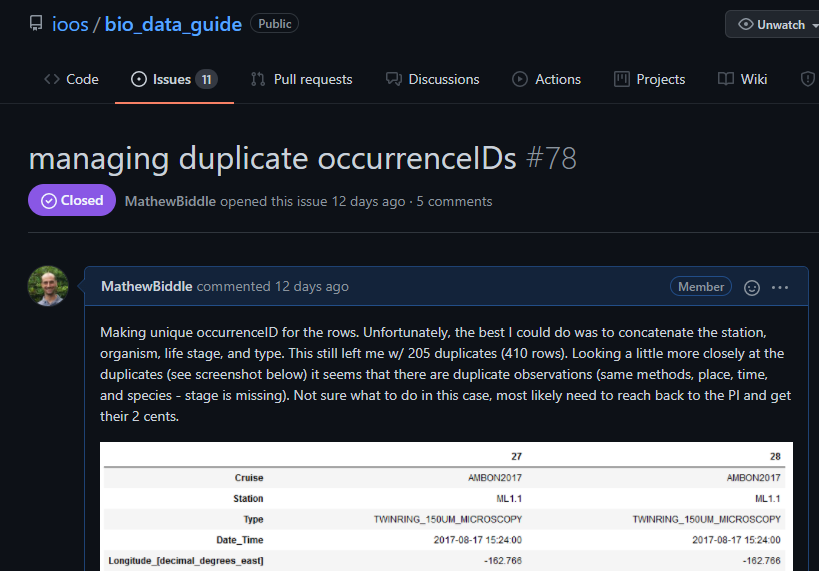
\includegraphics{./figs/issue_78.png}}
\item
  The data manager uploaded the raw data and code to GitHub through the pull request below. This included a fix for
  the \texttt{occurrenceID} issue.
  \href{https://github.com/ioos/bio_data_guide/pull/77}{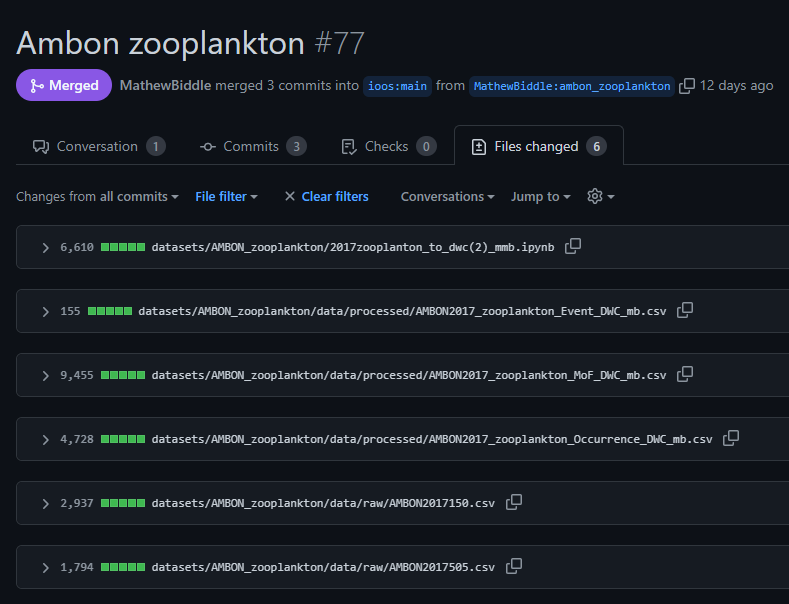
\includegraphics{./figs/PR_77.png}}
\item
  The OBIS node manager was notified of the availability of a revised dataset by pointing directly to the appropriate
  commit in GitHub:
  \href{https://github.com/ioos/bio_data_guide/commit/ef17f89f23316a6227fdf58de509582bd9854a55}{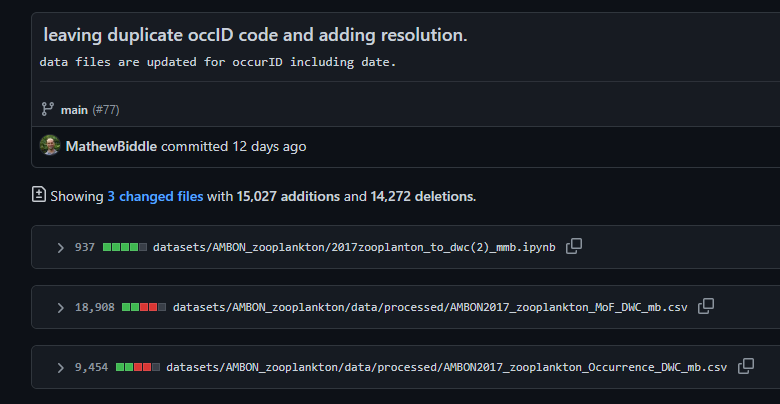
\includegraphics{./figs/commit_ef17f89.png}}
\item
  The OBIS node manager downloaded the data from the commit above and uploaded them to the IPT.
\item
  The IPT returned a summary of the dataset including that 434 records had invalid \texttt{scientificNameID} records in the
  occurrence file.
\item
  After some data sleuthing, the data manager noticed that the code accidentally removed trailing zeros from
  \texttt{scientificNameID} that ended in \texttt{0}:
  \href{https://nbviewer.org/github/ioos/bio_data_guide/blob/ef17f89f23316a6227fdf58de509582bd9854a55/datasets/AMBON_zooplankton/2017zooplanton_to_dwc\%282\%29_mmb.ipynb\#END-of-ID-generation}{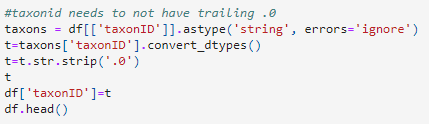
\includegraphics{./figs/code_snippet.png}}
\item
  So, the data manager updated the code to resolve the issue and generate a new occurrence file.
  \href{https://github.com/ioos/bio_data_guide/pull/82}{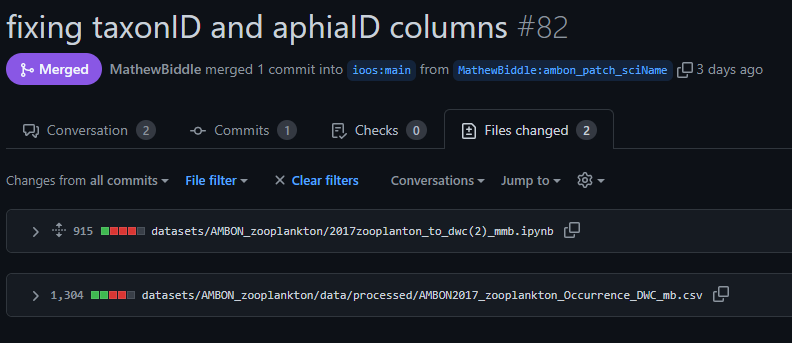
\includegraphics{./figs/PR_82.png}}

  \begin{enumerate}
  \def\labelenumii{\arabic{enumii}.}
  \tightlist
  \item
    Here is fixing the \texttt{scientificNameID} generation: 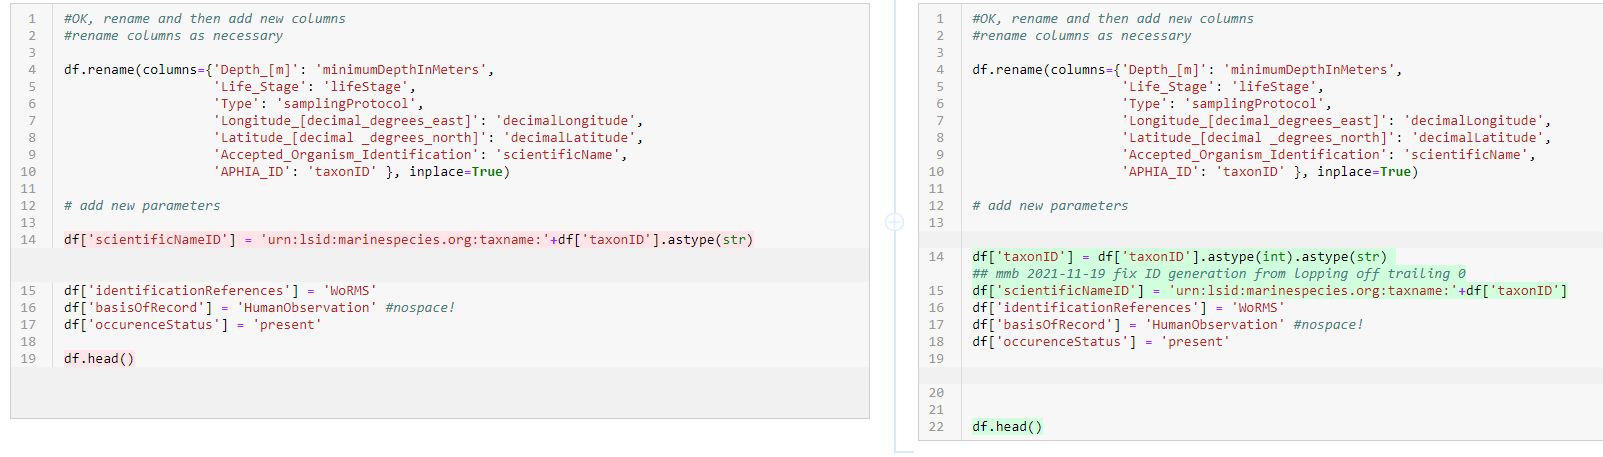
\includegraphics{./figs/code_change1.png}
  \item
    Here is removing the problematic code: 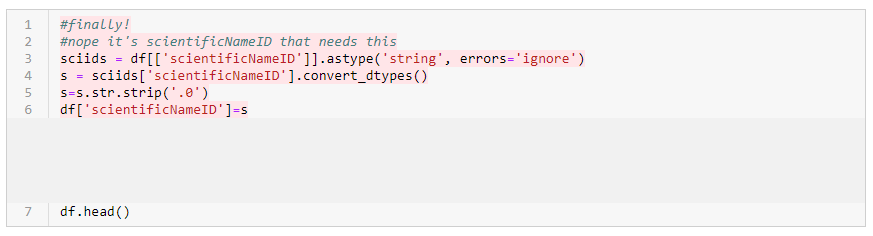
\includegraphics{./figs/code_change2.png} 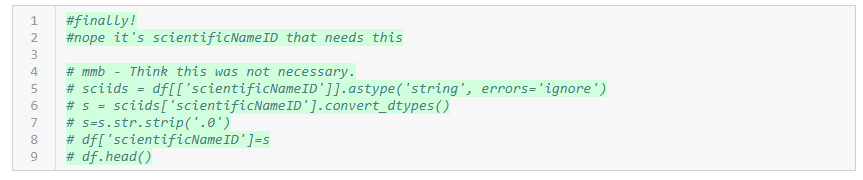
\includegraphics{./figs/code_change3.png}
  \end{enumerate}
\item
  The revised occurrence file was then resubmitted to the OBIS node manager by pointing them at the appropriate commit
  record:
  \href{https://github.com/ioos/bio_data_guide/commit/a0919e5b788b0737fc4c8e2c4b874c2e287769dd}{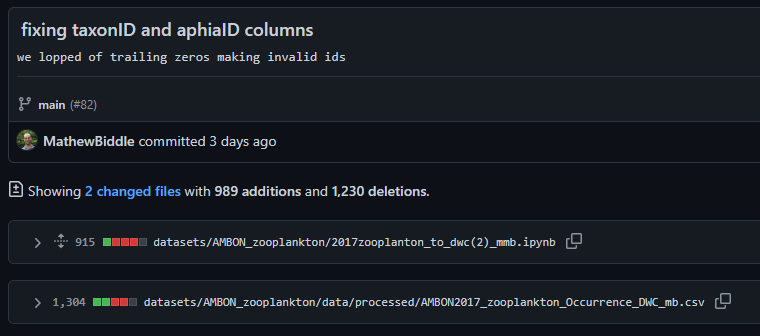
\includegraphics{./figs/commit_a0919e.png}}
\item
  The OBIS node manager downloaded the data from the commit above and uploaded them to the IPT.
\item
  The IPT and OBIS landing page now indicated that no more issues with these data are present:
  \href{https://obis.org/dataset/bc01451e-d990-4ad1-8315-e3fb6e9cf461}{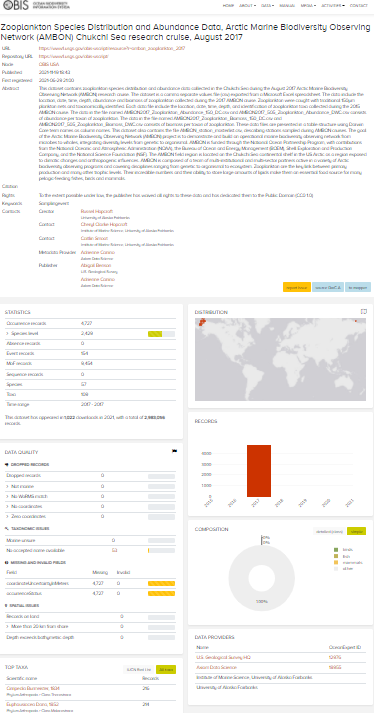
\includegraphics{./figs/obis_dataset.png}}
\end{enumerate}

\hypertarget{frequently-asked-questions}{%
\chapter{Frequently Asked Questions}\label{frequently-asked-questions}}

Q. What data structure does OBIS recommend?
A. The OBIS-ENV Darwin Core Archive Data Structure. \href{https://obis.org/manual/dataformat/\#envdata}{OBIS manual}

Q. What is a controlled vocabulary, why use them?
A. There are a number of controlled vocabularies that are used to describe parameters commonly used in specific research domains. Using terms defined in a controlled vocabulary allows for greater interoperability of data sets within the domain, and ideally between domains by ensuring that variables that are the same can be identified.

Q. What controlled vocabularies does OBIS rely on?
A. \href{https://www.marinespecies.org/}{WoRMS}, \href{http://vocab.nerc.ac.uk/}{NERC Vocabulary Server} inlcuding:
* \href{http://vocab.nerc.ac.uk/collection/L05/current/}{Device categories} using the SeaDataNet device categories

\begin{itemize}
\item
  \href{http://vocab.nerc.ac.uk/collection/L22/current/}{Device make/model using the SeaVoX Device Catalogue}
\item
  \href{http://vocab.nerc.ac.uk/collection/L06/current/}{Platform categories using SeaVoX Platform Categories}
\item
  \href{http://vocab.nerc.ac.uk/collection/C17/current/}{Platform instances using the ICES Platform Codes}
\item
  \href{http://vocab.nerc.ac.uk/collection/P06/current/}{Unit of measure}
\end{itemize}

Q. How can I find out which common measurementTypes are used in measurement or facts tables in existing OBIS datasets?
A. See \href{https://mof.obis.org/}{Measurement Types in OBIS}

Q. What is an ontology?
A. An ontology is a classification system for establishing a hierarchically related set of concepts. Concepts are often terms from controlled vocabularies. Ontologies can include all of the following, but are not required to include them.
Classes (general things, types of things)
Instances (individual things)
Relationships among things
Properties of things
Functions, processes, constraints, and rules relating to things

Q. What is ERDDAP?
A. \href{https://coastwatch.pfeg.noaa.gov/erddap/index.html}{ERDDAP} is a data server. It provides `easier access to scientific data' by providing a consistent interface that aggregates many disparate data sources. It does this by providing translation services between many common file types for gridded arrarys (`net CDF' files) and tabular data (spreadsheets). Data access is also made easier because it unifies different types of data servers and access protocols.

Q. What metadata profile does OBIS use?
A. OBIS uses the \href{http://rs.gbif.org/schema/eml-gbif-profile/1.1/eml-gbif-profile.xsd}{GBIF EML profile} (version 1.1)

Q. Can Darwin Core be used in the Semantic Web/Resrouce Description Framework?
A. See \href{https://dwc.tdwg.org/rdf/}{Darwin Core Resource Description Framework Guide} and
\href{http://www.semantic-web-journal.net/system/files/swj1093.pdf}{Lessons learned from adapting the Darwin Core vocabulary standard for use in RDF}

\hypertarget{tools}{%
\chapter{Tools}\label{tools}}

Below are some of the tools and packages used in workflows. R and Python package ``Type'' is BIO for packages specifically for biological applications, and GEN for generic packages.

\hypertarget{r}{%
\section{R}\label{r}}

\begin{longtable}[]{@{}
  >{\raggedright\arraybackslash}p{(\columnwidth - 4\tabcolsep) * \real{0.28}}
  >{\raggedright\arraybackslash}p{(\columnwidth - 4\tabcolsep) * \real{0.39}}
  >{\raggedright\arraybackslash}p{(\columnwidth - 4\tabcolsep) * \real{0.33}}@{}}
\toprule
\begin{minipage}[b]{\linewidth}\raggedright
Package
\end{minipage} & \begin{minipage}[b]{\linewidth}\raggedright
Type
\end{minipage} & \begin{minipage}[b]{\linewidth}\raggedright
Description
\end{minipage} \\
\midrule
\endhead
\href{https://bdverse.org/}{bdveRse} & BIO & A family of R packages for biodiversity data. \\
\href{https://cran.r-project.org/web/packages/ecocomDP/index.html}{ecocomDP} & BIO & Work with the Ecological Community Data Design Pattern. `ecocomDP' is a flexible data model for harmonizing ecological community surveys, in a research question agnostic format, from source data published across repositories, and with methods that keep the derived data up-to-date as the underlying sources change. \\
\href{https://ediorg.github.io/EMLassemblyline/}{EDIorg/EMLasseblyline} & BIO & For scientists and data managers to create high quality EML metadata for dataset publication. \\
\href{https://cran.r-project.org/web/packages/finch/index.html}{finch} & BIO & Parse Darwin Core Files \\
\href{https://iobis.github.io/obistools/}{iobis/obistools} & BIO & Tools for data enhancement and quality control. \\
\href{https://cran.r-project.org/web/packages/robis/index.html}{robis} & BIO & R client for the OBIS API \\
\href{https://docs.ropensci.org/EML/}{ropensci/EML} & BIO & Provides support for the serializing and parsing of all low-level EML concepts \\
\href{https://cran.r-project.org/web/packages/taxize/index.html}{taxize} & BIO & Interacts with a suite of web `APIs' for taxonomic tasks, such as getting database specific taxonomic identifiers, verifying species names, getting taxonomic hierarchies, fetching downstream and upstream taxonomic names, getting taxonomic synonyms, converting scientific to common names and vice versa, and more. \\
\href{https://cran.r-project.org/web/packages/worrms/index.html}{worrms} & BIO & Client for \href{http://www.marinespecies.org/}{World Register of Marine Species}. Includes functions for each of the API methods, including searching for names by name, date and common names, searching using external identifiers, fetching synonyms, as well as fetching taxonomic children and taxonomic classification. \\
\href{https://www.rdocumentation.org/packages/Hmisc/versions/4.6-0}{Hmisc} & GEN & Contains many functions useful for data analysis, high-level graphics, utility operations, functions for computing sample size and power, simulation, importing and annotating datasets, imputing missing values, advanced table making, variable clustering, character string manipulation, conversion of R objects to LaTeX and html code, and recoding variables. Particularly check out the \href{https://www.rdocumentation.org/packages/Hmisc/versions/4.6-0/topics/describe}{describe()} function. \\
\href{https://cran.r-project.org/web/packages/lubridate/index.html}{lubridate} & GEN & Functions to work with date-times and time-spans: fast and user friendly parsing of date-time data, extraction and updating of components of a date-time (years, months, days, hours, minutes, and seconds), algebraic manipulation on date-time and time-span objects. \\
\href{https://cran.r-project.org/web/packages/stringr/index.html}{stringr} & GEN & Simple, Consistent Wrappers for Common String Operations \\
\href{https://cran.r-project.org/web/packages/tidyverse/index.html}{tidyverse} & GEN & The `tidyverse' is a set of packages that work in harmony because they share common data representations and `API' design. This package is designed to make it easy to install and load multiple `tidyverse' packages in a single step. \\
\href{https://cran.r-project.org/web/packages/uuid/index.html}{uuid} & GEN & Tools for generating and handling of UUIDs (Universally Unique Identifiers). \\
\bottomrule
\end{longtable}

\hypertarget{python}{%
\section{Python}\label{python}}

\begin{longtable}[]{@{}
  >{\raggedright\arraybackslash}p{(\columnwidth - 4\tabcolsep) * \real{0.28}}
  >{\raggedright\arraybackslash}p{(\columnwidth - 4\tabcolsep) * \real{0.39}}
  >{\raggedright\arraybackslash}p{(\columnwidth - 4\tabcolsep) * \real{0.33}}@{}}
\toprule
\begin{minipage}[b]{\linewidth}\raggedright
Package
\end{minipage} & \begin{minipage}[b]{\linewidth}\raggedright
Type
\end{minipage} & \begin{minipage}[b]{\linewidth}\raggedright
Description
\end{minipage} \\
\midrule
\endhead
\href{https://pypi.org/project/metapype/}{metapype} & BIO & A lightweight Python 3 library for generating EML metadata \\
\href{https://python-dwca-reader.readthedocs.io/en/latest/index.html}{python-dwca-reader} & BIO & A simple Python package to read and parse Darwin Core Archive (DwC-A) files, as produced by the GBIF website, the IPT and many other biodiversity informatics tools. \\
\href{https://github.com/iobis/pyworms}{pyworms} & BIO & Python client for the World Register of Marine Species (WoRMS) REST service. \\
\href{https://numpy.org/}{numpy} & GEN & NumPy (Numerical Python) is an open source Python library that's used in almost every field of science and engineering. It's the universal standard for working with numerical data in Python, and it's at the core of the scientific Python and PyData ecosystems. \\
\href{https://pandas.pydata.org/}{pandas} & GEN & pandas is a fast, powerful, flexible and easy to use open source data analysis and manipulation tool, built on top of the Python programming language. Super helpful when manipulating tabular data! \\
\href{https://docs.python.org/3/library/uuid.html}{uuid} & GEN & This module provides immutable UUID objects (class UUID) and the functions uuid1(), uuid3(), uuid4(), uuid5() for generating version 1, 3, 4, and 5 UUIDs as specified in RFC 4122. Built in -- part of the Python standard library. \\
\href{https://github.com/iobis/obis-qc}{obis-qc} & BIO & Quality checks on occurrence records. Checks \texttt{occurrenceStatus}, \texttt{individualCount}, \texttt{eventDate}, \texttt{decimalLatitude}, \texttt{decimalLongitude}, \texttt{coordinateUncertaintyInMeters}, \texttt{minimumDepthInMeters}, \texttt{maximumDepthInMeters}, \texttt{scientificName}, \texttt{scientificNameID}. Checks from \href{https://www.ncbi.nlm.nih.gov/pmc/articles/PMC4309024/pdf/bau125.pdf}{Vandepitte et al.} flags not implemented: 3, 9, 14, 15, 16, 10, 17, 21-30. \\
\href{https://biopython.org/}{biopython} & BIO & Biopython is a set of freely available tools for biological computation written in Python by an international team of developers. It is a distributed collaborative effort to develop Python libraries and applications which address the needs of current and future work in bioinformatics. \\
\bottomrule
\end{longtable}

\hypertarget{google-sheets}{%
\section{Google Sheets}\label{google-sheets}}

\begin{longtable}[]{@{}
  >{\raggedright\arraybackslash}p{(\columnwidth - 2\tabcolsep) * \real{0.40}}
  >{\raggedright\arraybackslash}p{(\columnwidth - 2\tabcolsep) * \real{0.60}}@{}}
\toprule
\begin{minipage}[b]{\linewidth}\raggedright
Package
\end{minipage} & \begin{minipage}[b]{\linewidth}\raggedright
Description
\end{minipage} \\
\midrule
\endhead
\href{https://dwcaassistant.com/}{Google Sheet DarwinCore Archive Assistant add-on} & Google Sheet add-on which assists the creation of Darwin Core Archives (DwCA) and publising to Zenodo. DwCA's are stored into user's Google Drive and can be downloaded for upload into IPT installations or other software which is able to read DwC-archives. \\
\bottomrule
\end{longtable}

\hypertarget{validators}{%
\section{Validators}\label{validators}}

\begin{longtable}[]{@{}
  >{\raggedright\arraybackslash}p{(\columnwidth - 2\tabcolsep) * \real{0.29}}
  >{\raggedright\arraybackslash}p{(\columnwidth - 2\tabcolsep) * \real{0.71}}@{}}
\toprule
\begin{minipage}[b]{\linewidth}\raggedright
Name
\end{minipage} & \begin{minipage}[b]{\linewidth}\raggedright
Description
\end{minipage} \\
\midrule
\endhead
\href{https://tools.gbif.org/dwca-validator/}{Darwin Core Archive Validator} & This validator verifies the structural integrity of a Darwin Core Archive. It does not check the data values, such as coordinates, dates or scientific names. \\
\href{https://www.gbif.org/tools/data-validator}{GBIF DATA VALIDATOR} & The GBIF data validator is a service that allows anyone with a GBIF-relevant dataset to receive a report on the syntactical correctness and the validity of the content contained within the dataset. \\
\href{https://www.lifewatch.be/data-services/}{LifeWatch Belgium} & Through this interactive section of the LifeWatch.be portal users can upload their own data using a standard data format, and choose from several web services, models and applications to process the data. \\
\bottomrule
\end{longtable}

\hypertarget{extras}{%
\chapter{Extras}\label{extras}}

Below is some more in-depth information into specific areas associated with standardizing your data to Darwin Core and uploading it through the IPT.

\hypertarget{ecological-metadata-language-eml}{%
\section{Ecological Metadata Language (EML)}\label{ecological-metadata-language-eml}}

The Ecological Metadata Language (EML) is a community developed and maintained metadata standard that is typically associated with ecological-, and earth and environmental data. The purpose of EML is to provide the ecological community with an extensible, flexible, metadata standard used in data analysis and archiving, which will allow automated machine processing, searching and retrieval. EML has been around since 2003, and can be considered a ``dialect'' or specification to XML to describe tables and other data objects. The XML Schema provides a framework for the metadata, with defined ``rules'' on how to organize the metadata without any stipulations (another way to put it, \emph{XML is the language that defines the rules that govern the EML syntax}). The XML Schema defines the structure of some information in a document (e.g.~elements and attributes names and relationships), but does not provide any specific details the information included within. An EML document or file (eml.xml) is used to provide detailed description of metadata related to data objects, including tables (and other data objects), their columns, typing etc, and how data tables are linked or grouped. EML is widely used for datasets about ecosystem level observations, and can be used to detail data table information to a high granularity, which allows data users to arrange data tables in any way they need to. EML is particularly useful for wide data tables as table level details are entirely contained within the metadata document, meaning that there is not necessarily a need for external definitions such as a code list. However, if you have a long table arrangement, like the Darwin Core Archive (DwC-A), you can define the allowable values for the column in the metadata as well.

EML is excellent at describing the details of a column of data so that the data values in the tables can be read into analysis systems or an analysis environment using the metadata, or even into a relational database. EML allows for tables to be easily reusable, and read into workflows, translated or reformatted. A drawback to EML is that, compared to the ISO standard, EML is a community standard, adopting a more `bottom-up' approach. This is contrary to the ISO standard, which are internationally agreed upon standards by experts (`top-down'). However, at the time of EML development in the early 2000's there was a gap in metadata options to describe ecological data tables, with ISO standards typically being more applicable to geographic data. EML can cover almost anything and is particularly good at tabular data. But at the same time, due to the self-contained nature, there can be little control from outside lists, which means that the description is left to the EML constructor (data provider/manager) and consequently, individual datasets can look quite different from each other, even when they contain similar measurements. As such, it will be important to document best practices and clear mapping of fields between different metadata schemas (e.g.~cross-walks between ISO.xml and EML.xml). As of version 2.2, EML can link to external ontologies, and there is capacity for annotation with external terms (e.g.~through their URIs). Code lists and external dictionaries can help as they sometimes contain additional information that might not fit into EML (e.g.~protocols, or code lists stored in ontologies). Having these external code lists and exporting them as EML snippets could go a long way in reducing that heterogeneity, because the constructors can then select measurements from lists when developing EML documents.

EML is implemented as a series of XML document types (modules) that can be used in an extensible manner to document ecological data. Each EML module is designed to describe one logical part of the total metadata that should be included with any ecological dataset. The architecture of EML was designed to serve the needs of the ecological community, and has benefitted from previous work in other related metadata standards. Using this format can facilitate future growth of the metadata language, and EML supports an active developer community (see e.g.~NCEAS EML GitHub). EML adopts much of its syntax from the other metadata standards that have evolved from the expertise of groups in other disciplines. Whenever possible, EML adopted entire trees of information in order to facilitate conversion of EML documents into other metadata languages. The GBIF IPT is a tool used to create a single eml.xml file format inside the DwC-A data package. However, the IPT does not use any of the EML's built-in table description modules, and perhaps primarily uses one EML module (resource module) for high-level metadata.

However, it is important to know how both OBIS and GBIF use EML, as often a higher granularity of the metadata can be found in the original data tables. An example of this is spatial coverage. The IPT only allows for either a bounding box to be documented (populating North, South, East, and West coordinates), or a single polygon. The EML document however would be able to capture multiple polygons worth of spatial coverage (i.e.~a polygon for each transect surveyed). This more detailed information however is often captured in the data (in an OBIS record). Additionally, not all fields that can be populated in an EML document can be translated to the IPT, or harvested by OBIS and GBIF. The GBIF IPT only produces a select number of fields or attributes available in EML.

\emph{Important}: When reading the EML section in the \href{https://obis.org/manual/eml/}{OBIS manual}, you'll notice that it reads that OBIS uses the GBIF EML profile (version 1.1). However, the current EML version is 2.2.0, as per \href{https://eml.ecoinformatics.org/}{EcoInformatics}. This does not mean that these versions are not compatible, rather, it means that the GBIF IPT currently uses a subset of available EML 2.2.0 fields and attributes, the subset of which they have versioned 1.1.

If you are interested in creating an EML metadata file, it is possible to upload those into the IPT. There are R packages that can help in developing an EML.xml file. These packages are e.g.~\href{https://github.com/ropensci/EML}{EML}, \href{https://github.com/ropensci/emld}{emld} or \href{https://ediorg.github.io/EMLassemblyline/articles/overview.html}{EMLassemblyline}.

\hypertarget{references}{%
\chapter*{References}\label{references}}
\addcontentsline{toc}{chapter}{References}

\setlength{\parindent}{-0.2in}
\setlength{\leftskip}{0.2in}
\setlength{\parskip}{8pt}

\noindent

\hypertarget{refs}{}
\begin{CSLReferences}{1}{0}
\leavevmode\vadjust pre{\hypertarget{ref-R-rmarkdown}{}}%
Allaire, JJ, Yihui Xie, Jonathan McPherson, Javier Luraschi, Kevin Ushey, Aron Atkins, Hadley Wickham, Joe Cheng, Winston Chang, and Richard Iannone. 2022. \emph{Rmarkdown: Dynamic Documents for r}. \url{https://CRAN.R-project.org/package=rmarkdown}.

\leavevmode\vadjust pre{\hypertarget{ref-Barbier2017}{}}%
Barbier, Edward B. 2017. {``Marine Ecosystem Services.''} \emph{Current Biology}. Cell Press. \url{https://doi.org/10.1016/j.cub.2017.03.020}.

\leavevmode\vadjust pre{\hypertarget{ref-Benson2018}{}}%
Benson, Abigail, Cassandra M. Brooks, Gabrielle Canonico, Emmett Duffy, Frank Muller-Karger, Heidi M. Sosik, Patricia Miloslavich, and Eduardo Klein. 2018. {``Integrated Observations and Informatics Improve Understanding of Changing Marine Ecosystems.''} \emph{Frontiers in Marine Science}. Frontiers Media S.A. \url{https://doi.org/10.3389/fmars.2018.00428}.

\leavevmode\vadjust pre{\hypertarget{ref-benson_lascala-gruenewald_mcguinn_satterthwaite_beaulieu_biddle_dewitt_mckinzie_montes_moustahfid_etal_2021}{}}%
Benson, Abigail, Diana LaScala-Gruenewald, Robert McGuinn, Erin Satterthwaite, Stace Beaulieu, Mathew Biddle, Lynn deWitt, et al. 2021. {``Biological Observation Data Standardization - a Primer for Data Managers.''} ESIP. \url{https://doi.org/10.6084/m9.figshare.16806712.v1}.

\leavevmode\vadjust pre{\hypertarget{ref-article}{}}%
Benson, Abigail, Tylar Murray, Gabrielle Canonico, Enrique Montes, Frank Muller-Karger, Maria T. Kavanaugh, Joaquin Trinanes, and Lynn M. deWitt. 2021. {``Data Management and Interactive Visualizations for the Evolving Marine Biodiversity Observation Network.''} \emph{Oceanography}. \url{https://doi.org/10.5670/oceanog.2021.220}.

\leavevmode\vadjust pre{\hypertarget{ref-Borer2009}{}}%
Borer, Elizabeth T., Eric W. Seabloom, Matthew B. Jones, and Mark Schildhauer. 2009. {``Some Simple Guidelines for Effective Data Management.''} \emph{Bulletin of the Ecological Society of America} 90 (April). \url{https://doi.org/10.1890/0012-9623-90.2.205}.

\leavevmode\vadjust pre{\hypertarget{ref-Canonico2019}{}}%
Canonico, Gabrielle, Pier Luigi Buttigieg, Enrique Montes, Frank E. Muller-Karger, Carol Stepien, Dawn Wright, Abigail Benson, et al. 2019. {``Global Observational Needs and Resources for Marine Biodiversity.''} \emph{Frontiers in Marine Science}. Frontiers Media S.A. \url{https://doi.org/10.3389/fmars.2019.00367}.

\leavevmode\vadjust pre{\hypertarget{ref-Crystal-Ornela2021}{}}%
Crystal-Ornelas, Robert, Charuleka Varadharajan, Ben Bond-Lamberty, Kristin Boye, Madison Burrus, Shreyas Cholia, Michael Crow, et al. 2021. {``A Guide to Using GitHub for Developing and Versioning Data Standards and Reporting Formats.''} \emph{Earth and Space Science}, July, e2021EA001797. \url{https://doi.org/10.1029/2021EA001797}.

\leavevmode\vadjust pre{\hypertarget{ref-Davies2021}{}}%
Davies, Neil, John Deck, Eric C Kansa, Sarah Whitcher Kansa, John Kunze, Christopher Meyer, Thomas Orrell, et al. 2021. {``Internet of Samples (iSamples): Toward an Interdisciplinary Cyberinfrastructure for Material Samples.''} \emph{GigaScience} 10: 1--5. \url{https://doi.org/10.1093/gigascience/giab028}.

\leavevmode\vadjust pre{\hypertarget{ref-Djurhuus2020}{}}%
Djurhuus, Anni, Collin J. Closek, Ryan P. Kelly, Kathleen J. Pitz, Reiko P. Michisaki, Hilary A. Starks, Kristine R. Walz, et al. 2020. {``Environmental DNA Reveals Seasonal Shifts and Potential Interactions in a Marine Community.''} \emph{Nature Communications} 11 (December): 1--9. \url{https://doi.org/10.1038/s41467-019-14105-1}.

\leavevmode\vadjust pre{\hypertarget{ref-Duffy2013}{}}%
Duffy, J. Emmett, Linda A. Amaral-Zettler, Daphne G. Fautin, Gustav Paulay, Tatiana A. Rynearson, Heidi M. Sosik, and John J. Stachowicz. 2013. {``Envisioning a Marine Biodiversity Observation Network.''} \emph{BioScience} 63 (May): 350--61. \url{https://doi.org/10.1525/bio.2013.63.5.8}.

\leavevmode\vadjust pre{\hypertarget{ref-Fornwall2012}{}}%
Fornwall, M, R Gisiner, S E Simmons, H Moustahfid, G Canonico, P Halpin, P Goldstein, et al. 2012. {``Expanding Biological Data Standards Development Processes for US IOOS: Visual Line Transect Observing Community for Mammal, Bird, and Turtle Data.''} IOOS. \url{https://www.researchgate.net/publication/255681522}.

\leavevmode\vadjust pre{\hypertarget{ref-Hardisty2019}{}}%
Hardisty, Alex R., William K. Michener, Donat Agosti, Enrique Alonso García, Lucy Bastin, Lee Belbin, Anne Bowser, et al. 2019. {``The Bari Manifesto: An Interoperability Framework for Essential Biodiversity Variables.''} \emph{Ecological Informatics} 49 (January): 22--31. \url{https://doi.org/10.1016/j.ecoinf.2018.11.003}.

\leavevmode\vadjust pre{\hypertarget{ref-Heberling2021}{}}%
Heberling, J Mason, Joseph T Miller, Daniel Noesgaard, Scott B Weingart C, Dmitry Schigel, and Douglas E Soltis. 2021. {``Data Integration Enables Global Biodiversity Synthesis.''} \emph{Proceedings of the National Academy of Sciences of the United States of America}. \url{https://doi.org/10.1073/pnas.2018093118/-/DCSupplemental}.

\leavevmode\vadjust pre{\hypertarget{ref-Hare2016PLOS}{}}%
Jonathan A. Hare, Mark W. Nelson, Wendy E. Morrison. n.d. {``A Vulnerability Assessment of Fish and Invertebrates to Climate Change on the Northeast u.s. Continental Shelf.''} \emph{PLoS ONE} 11 (2): e0146756. \url{https://doi.org/10.1371/journal.pone.0146756}.

\leavevmode\vadjust pre{\hypertarget{ref-Jones2006}{}}%
Jones, Matthew B., Mark P. Schildhauer, O. J. Reichman, and Shawn Bowers. 2006. {``The New Bioinformatics: Integrating Ecological Data from the Gene to the Biosphere.''} \emph{Annual Review of Ecology, Evolution, and Systematics}. \url{https://doi.org/10.1146/annurev.ecolsys.37.091305.110031}.

\leavevmode\vadjust pre{\hypertarget{ref-Kavanaugh2016}{}}%
Kavanaugh, Maria T., Matthew J. Oliver, Francisco P. Chavez, Ricardo M. Letelier, Frank E. Muller-Karger, and Scott C. Doney. 2016. {``Seascapes as a New Vernacular for Pelagic Ocean Monitoring, Management and Conservation.''} \emph{ICES Journal of Marine Science} 73 (July): 1839--50. \url{https://doi.org/10.1093/icesjms/fsw086}.

\leavevmode\vadjust pre{\hypertarget{ref-Kot2010}{}}%
Kot, Connie Y., Ei Fujioka, Lucie J. Hazen, Benjamin D. Best, Andrew J. Read, and Patrick N. Halpin. 2010. {``Spatio-Temporal Gap Analysis of OBIS-SEAMAP Project Data: Assessment and Way Forward.''} \emph{PLoS ONE} 5 (September): 12990. \url{https://doi.org/10.1371/journal.pone.0012990}.

\leavevmode\vadjust pre{\hypertarget{ref-OceanAdapt}{}}%
Lab, Malin Pinksy. n.d. {``OceanAdapt.''} \emph{GitHub}. \url{https://oceanadapt.rutgers.edu/}.

\leavevmode\vadjust pre{\hypertarget{ref-Lamprecht2019}{}}%
Lamprecht, Anna-Lena, Leyla Garcia, Mateusz Kuzak, Carlos Martinez, Ricardo Arcila, Eva Martin Del Pico, Victoria Dominguez Del Angel, et al. 2019. {``Towards FAIR Principles for Research Software.''} Edited by Paul Groth. \emph{Data Science}, 1--23. \url{https://doi.org/10.3233/DS-190026}.

\leavevmode\vadjust pre{\hypertarget{ref-Dornelas2014Science}{}}%
Maria Dornelas, Brian McGill, Nicholas J. Gotelli. 2014. {``Assemblage Time Series Reveal Biodiversity Change but Not Systematic Loss.''} \emph{Science} 344 (6181): 296--99. \url{https://doi.org/10.1126/science.1248484}.

\leavevmode\vadjust pre{\hypertarget{ref-McKenna2021}{}}%
McKenna, Megan F., Simone Baumann-Pickering, Annebelle C. M. Kok, William K. Oestreich, Jeffrey D. Adams, Jack Barkowski, Kurt M. Fristrup, et al. 2021. {``Advancing the Interpretation of Shallow Water Marine Soundscapes.''} \emph{Frontiers in Marine Science} 0 (September): 1426. \url{https://doi.org/10.3389/FMARS.2021.719258}.

\leavevmode\vadjust pre{\hypertarget{ref-Miloslavich2018}{}}%
Miloslavich, Patricia, Nicholas J. Bax, Samantha E. Simmons, Eduardo Klein, Ward Appeltans, Octavio Aburto-Oropeza, Melissa Andersen Garcia, et al. 2018. {``Essential Ocean Variables for Global Sustained Observations of Biodiversity and Ecosystem Changes.''} \emph{Global Change Biology} 24 (June): 2416--33. \url{https://doi.org/10.1111/gcb.14108}.

\leavevmode\vadjust pre{\hypertarget{ref-Montes2020}{}}%
Montes, Enrique, Anni Djurhuus, Frank E. Muller-Karger, Daniel Otis, Christopher R. Kelble, and Maria T. Kavanaugh. 2020. {``Dynamic Satellite Seascapes as a Biogeographic Framework for Understanding Phytoplankton Assemblages in the Florida Keys National Marine Sanctuary, United States.''} \emph{Frontiers in Marine Science} 7 (July): 575. \url{https://doi.org/10.3389/fmars.2020.00575}.

\leavevmode\vadjust pre{\hypertarget{ref-Moustahfid2014}{}}%
Moustahfid, Hassan, and Philip Goldstein. 2014. {``IOOS Biological Data Services Enrollment Procedures.''}

\leavevmode\vadjust pre{\hypertarget{ref-Moustahfid2011}{}}%
Moustahfid, Hassan, Jim Potemra, Philip Goldstein, Roy Mendelssohn, and Annette Desrochers. 2011. {``Making United States Integrated Ocean Observing System (u.s. IOOS) Inclusive of Marine Biological Resources.''} \url{https://www.researchgate.net/publication/254013004}.

\leavevmode\vadjust pre{\hypertarget{ref-Muller-Karger2018b}{}}%
Muller-Karger, Frank E., Erin Hestir, Christiana Ade, Kevin Turpie, Dar A. Roberts, David Siegel, Robert J. Miller, et al. 2018. {``Satellite Sensor Requirements for Monitoring Essential Biodiversity Variables of Coastal Ecosystems.''} \emph{Ecological Applications} 28 (April): 749--60. \url{https://doi.org/10.1002/eap.1682}.

\leavevmode\vadjust pre{\hypertarget{ref-Muller-Karger2018a}{}}%
Muller-Karger, Frank E., Patricia Miloslavich, Nicholas J. Bax, Samantha Simmons, Mark J. Costello, Isabel Sousa Pinto, Gabrielle Canonico, et al. 2018. {``Advancing Marine Biological Observations and Data Requirements of the Complementary Essential Ocean Variables (EOVs) and Essential Biodiversity Variables (EBVs) Frameworks.''} \emph{Frontiers in Marine Science}. Frontiers Media S.A. \url{https://doi.org/10.3389/fmars.2018.00211}.

\leavevmode\vadjust pre{\hypertarget{ref-Neeley2021}{}}%
Neeley, Aimee, Stace E. Beaulieu, Chris Proctor, Ivona Cetinić, Joe Futrelle, Inia Soto Ramos, Heidi M. Sosik, et al. 2021. {``Standards and Practices for Reporting Plankton and Other Particle Observations from Images.''} \url{https://doi.org/10.1575/1912/27377}.

\leavevmode\vadjust pre{\hypertarget{ref-Obrien2021}{}}%
O'Brien, Margaret, Colin A. Smith, Eric R. Sokol, Corinna Gries, Nina Lany, Sydne Record, and Max C. N. Castorani. 2021. {``ecocomDP: A Flexible Data Design Pattern for Ecological Community Survey Data.''} \emph{Ecological Informatics} 64 (September): 101374. \url{https://doi.org/10.1016/J.ECOINF.2021.101374}.

\leavevmode\vadjust pre{\hypertarget{ref-Pooter2017}{}}%
Pooter, Daphnis De, Ward Appeltans, Nicolas Bailly, Sky Bristol, Klaas Deneudt, Menashè Eliezer, Ei Fujioka, et al. 2017. {``Toward a New Data Standard for Combined Marine Biological and Environmental Datasets - Expanding OBIS Beyond Species Occurrences.''} \emph{Biodiversity Data Journal} 5 (January): 10989. \url{https://doi.org/10.3897/BDJ.5.e10989}.

\leavevmode\vadjust pre{\hypertarget{ref-iobis_ebsa}{}}%
Provoost, Pieter. n.d. {``Iobis/Ebsa.''} \emph{GitHub}. \url{https://github.com/iobis/ebsa}.

\leavevmode\vadjust pre{\hypertarget{ref-R-base}{}}%
R Core Team. 2021. \emph{R: A Language and Environment for Statistical Computing}. Vienna, Austria: R Foundation for Statistical Computing. \url{https://www.R-project.org/}.

\leavevmode\vadjust pre{\hypertarget{ref-Ruxfccknagel2015}{}}%
Rücknagel, J., P. Vierkant, R. Ulrich, G. Kloska, E. Schnepf, D. Fichtmüller, E. Reuter, et al. 2015. {``Metadata Schema for the Description of Research Data Repositories. Version 3.0.''} \url{https://doi.org/10.2312/re3.008}.

\leavevmode\vadjust pre{\hypertarget{ref-Rule2019}{}}%
Rule, Adam, Amanda Birmingham, Cristal Zuniga, Ilkay Altintas, Shih-Cheng Huang, Rob Knight, Niema Moshiri, et al. 2019. {``Ten Simple Rules for Writing and Sharing Computational Analyses in Jupyter Notebooks.''} \emph{PLOS Computational Biology} 15 (July): e1007007. \url{https://doi.org/10.1371/JOURNAL.PCBI.1007007}.

\leavevmode\vadjust pre{\hypertarget{ref-Santora2017}{}}%
Santora, Jarrod A., Elliott L. Hazen, Isaac D. Schroeder, Steven J. Bograd, Keith M. Sakuma, and John C. Field. 2017. {``Impacts of Ocean Climate Variability on Biodiversity of Pelagic Forage Species in an Upwelling Ecosystem.''} \emph{Marine Ecology Progress Series} 580 (September): 205--20. \url{https://doi.org/10.3354/meps12278}.

\leavevmode\vadjust pre{\hypertarget{ref-Schmid_Daprano_Jacobson_Sullivan_Briseuxf1o-Avena_Luo_Cowen_2021}{}}%
Schmid, Moritz S, Dominic Daprano, Kyler M Jacobson, Christopher Sullivan, Christian Briseño-Avena, Jessica Y Luo, and Robert K Cowen. 2021. \emph{A Convolutional Neural Network Based High-Throughput Image Classification Pipeline - Code and Documentation to Process Plankton Underwater Imagery Using Local HPC Infrastructure and NSF's XSEDE}. Zenodo. \url{https://doi.org/10.5281/ZENODO.4641158}.

\leavevmode\vadjust pre{\hypertarget{ref-Taylor2012}{}}%
Taylor, Gordon T., Frank E. Muller-Karger, Robert C. Thunell, Mary I. Scranton, Yrene Astor, Ramon Varela, Luis Troccoli Ghinaglia, et al. 2012. {``Ecosystem Responses in the Southern Caribbean Sea to Global Climate Change.''} \emph{Proceedings of the National Academy of Sciences of the United States of America} 109 (November): 19315--20. \url{https://doi.org/10.1073/pnas.1207514109}.

\leavevmode\vadjust pre{\hypertarget{ref-tittensor2010global}{}}%
Tittensor, Derek P, Camilo Mora, Walter Jetz, Heike K Lotze, Daniel Ricard, Edward Vanden Berghe, and Boris Worm. 2010. {``Global Patterns and Predictors of Marine Biodiversity Across Taxa.''} \emph{Nature} 466 (7310): 1098.

\leavevmode\vadjust pre{\hypertarget{ref-Warren2018}{}}%
Warren, R., J. Price, E. Graham, N. Forstenhaeusler, and J. VanDerWal. 2018. {``The Projected Effect on Insects, Vertebrates, and Plants of Limiting Global Warming to 1.5°c Rather Than 2°c.''} \emph{Science} 360 (May): 791--95. \url{https://doi.org/10.1126/science.aar3646}.

\leavevmode\vadjust pre{\hypertarget{ref-Wieczorek2012}{}}%
Wieczorek, John, David Bloom, Robert Guralnick, Stan Blum, Markus Döring, Renato Giovanni, Tim Robertson, and David Vieglais. 2012. {``Darwin Core: An Evolving Community-Developed Biodiversity Data Standard.''} \emph{PLoS ONE} 7 (January): 29715. \url{https://doi.org/10.1371/journal.pone.0029715}.

\leavevmode\vadjust pre{\hypertarget{ref-Wilkinson2016}{}}%
Wilkinson, Mark D., Michel Dumontier, IJsbrand Jan Aalbersberg, Gabrielle Appleton, Myles Axton, Arie Baak, Niklas Blomberg, et al. 2016. {``The FAIR Guiding Principles for Scientific Data Management and Stewardship.''} \emph{Scientific Data} 3 (March): 1--9. \url{https://doi.org/10.1038/sdata.2016.18}.

\leavevmode\vadjust pre{\hypertarget{ref-knitr2014}{}}%
Xie, Yihui. 2014. {``Knitr: A Comprehensive Tool for Reproducible Research in {R}.''} In \emph{Implementing Reproducible Computational Research}, edited by Victoria Stodden, Friedrich Leisch, and Roger D. Peng. Chapman; Hall/CRC. \url{http://www.crcpress.com/product/isbn/9781466561595}.

\leavevmode\vadjust pre{\hypertarget{ref-xie2015}{}}%
---------. 2015b. \emph{Dynamic Documents with {R} and Knitr}. 2nd ed. Boca Raton, Florida: Chapman; Hall/CRC. \url{http://yihui.name/knitr/}.

\leavevmode\vadjust pre{\hypertarget{ref-knitr2015}{}}%
---------. 2015a. \emph{Dynamic Documents with {R} and Knitr}. 2nd ed. Boca Raton, Florida: Chapman; Hall/CRC. \url{https://yihui.org/knitr/}.

\leavevmode\vadjust pre{\hypertarget{ref-bookdown2016}{}}%
---------. 2016. \emph{Bookdown: Authoring Books and Technical Documents with {R} Markdown}. Boca Raton, Florida: Chapman; Hall/CRC. \url{https://bookdown.org/yihui/bookdown}.

\leavevmode\vadjust pre{\hypertarget{ref-R-bookdown}{}}%
---------. 2022a. \emph{Bookdown: Authoring Books and Technical Documents with r Markdown}. \url{https://CRAN.R-project.org/package=bookdown}.

\leavevmode\vadjust pre{\hypertarget{ref-R-knitr}{}}%
---------. 2022b. \emph{Knitr: A General-Purpose Package for Dynamic Report Generation in r}. \url{https://yihui.org/knitr/}.

\leavevmode\vadjust pre{\hypertarget{ref-rmarkdown2018}{}}%
Xie, Yihui, J. J. Allaire, and Garrett Grolemund. 2018. \emph{R Markdown: The Definitive Guide}. Boca Raton, Florida: Chapman; Hall/CRC. \url{https://bookdown.org/yihui/rmarkdown}.

\leavevmode\vadjust pre{\hypertarget{ref-rmarkdown2020}{}}%
Xie, Yihui, Christophe Dervieux, and Emily Riederer. 2020. \emph{R Markdown Cookbook}. Boca Raton, Florida: Chapman; Hall/CRC. \url{https://bookdown.org/yihui/rmarkdown-cookbook}.

\end{CSLReferences}

\end{document}
